%%
\documentclass[11pt,a4paper,english,greek,twoside]{ceid-thesis}

\usepackage{graphicx}
\usepackage{epstopdf}
\usepackage{indentfirst}
\usepackage{verbatim}
\usepackage{amsmath}
\usepackage{amsthm}
\usepackage{amssymb}
\usepackage{latexsym}
\bibliographystyle{pictures/hellas}
\usepackage{hyphenat}
\usepackage{makeidx}
% next 3 lines: addition to use greek in bibliography
\usepackage[LGR,T1]{fontenc}
\usepackage[utf8]{inputenc}
\usepackage{textalpha}
\addto\captionsgreek{%
  \renewcommand{\indexname}{Ευρετήριο όρων}%
}
\makeindex

% 1.5 spacing
\renewcommand{\baselinestretch}{1.2}

% latin text (and greek text)
\newcommand{\tl}[1]{\textlatin{#1}}
\newcommand{\tg}[1]{\textgreek{#1}}

% typeset short english phrases
\newcommand{\en}[1]{\foreignlanguage{english}{#1}}

% typeset source code
\newcommand{\src}[1]{{\tt\en{#1}}}

% typeset a backslash
\newcommand{\bkslash}{\en{\symbol{92}}}

\newtheorem{definition}{Ορισμός}
\newtheorem{proposition}{Πρόταση}
\newtheorem{theorem}{Θεώρημα}
\newtheorem{corollary}{Συμπέρασμα}
\newtheorem{lemma}{Λήμμα}
\newtheorem{example}{Παράδειγμα}
\newtheorem{remark}{Σημείωση}
\newtheorem{notation}{Συμβολισμός}
\newtheorem{law}{Νόμος}
\renewcommand{\thedefinition}{\arabic{chapter}.\arabic{definition}}
\renewcommand{\theproposition}{\arabic{chapter}.\arabic{proposition}}
\renewcommand{\thetheorem}{\arabic{chapter}.\arabic{theorem}}
\renewcommand{\thecorollary}{\arabic{chapter}.\arabic{corollary}}
\renewcommand{\thelemma}{\arabic{chapter}.\arabic{lemma}}
\renewcommand{\theexample}{\arabic{chapter}.\arabic{example}}
\newcommand{\set}[1]{\left\{#1\right\}}
\newcommand{\To}{\Longrightarrow}
\newcommand{\xml}{\en{XML}}

\selectlanguage{greek}

\hyphenation{ο-ποί-α}

%%%%%%%%%%%%%%%%%%%%%%%%%%%%%%%%%%%%%%%%%%%%%%%%%%%%%
%% THESIS INFO 
%%
%
% Τίτλος Πτυχιακής Εργασίας
	\title{Μέθοδοι Μηχανικής Μάθησης στον χώρο της Ιατρικής Φροντίδας \tl{(Healthcare)}}
% "του" ή "της", ανάλογα με το φύλο του σπουδαστή
	\edef\toutis{του}
% Ονοματεπώνυμο σπουδαστή (ΚΕΦΑΛΑΙΑ, γενική πτώση)
	\edef\authorNameCapital{ΔΗΜΗΤΡΙΟΥ ΚΑΡΑΜΑΝΗ}
% Ονοματεπώνυμο σπουδαστή (πεζά, ονομαστική πτώση)
	\author{Δημήτριος Καραμάνης}
% Ονοματεπώνυμο Επιβλέποντα Καθηγητή
	\supervisor{Χρήστος Μακρής}
    \edef\supervisorTitle{Αναπληρωτής Καθηγητής}
% Ονοματεπώνυμο Επιβλέποντα Καθηγητή
	\supervisorSecond{}
    \edef\supervisorSecondTitle{**** Τιτλος}

% "Επιβλέπων" ή "Επιβλέπουσα", ανάλογα με το φύλο του Επιβλέποντα Καθηγητή
	\edef\supervisorMaleFemale{Επιβλέποντες}
% Τόπος, μήνας και έτος
	\edef\thesisPlaceDate{Πατρα, Ιούνιος 2023}
% Ημερομηνία Εξέτασης
	\edef\examinationDate{χχ Ιουνίου 2023}
% Έτος Copyright
	\edef\copyrightYear{2023}
% Ονοματεπώνυμο 1ου εξεταστή
	\epitropiF{Σπύρος Σιούτας}
% Τίτλος 1ου εξεταστή
	\edef\epitropiFTitle{Καθηγητής}
% Ονοματεπώνυμο 2ου εξεταστή
	\epitropiS{Δημήτριος Τσώλης}
% τίτλος 2ου εξεταστή
	\edef\epitropiSTitle{Επίκουρος Καθηγητής}
%%%%%%%%%%%%%%%%%%%%%%%%%%%%%%%%%%%%%%%%%%%%%%%%%%%%%
%=========== APOTROPI SULLAVISMOU
\tolerance=1
\emergencystretch=\maxdimen
\hyphenpenalty=10000
\hbadness=10000

\begin{document}
\selectlanguage{greek}
\maketitle

\frontmatter
% Περίληψη
	\begin{abstract}
Η εκπαίδευση ενός υπολογιστικού συστήματος στην νοηματική αναγνώριση κειμένου και την εξαγωγή συμπερασμάτων από αυτό, αποτελεί μια πρόκληση για την επιστημονική κοινότητα και την έρευνα.

Στόχος του συγκεκριμένου ερευνητικού πεδίου που δημιουργήθηκε από αυτήν την πρόκληση είναι η δημιουργία κατάλληλων εργαλείων για την υποστήριξη, υποβοήθηση και διευκόλυνση του ανθρώπινου δυναμικού.

Στην παρούσα διπλωματική εργασία δίνεται έμφαση στην χρήση ιατρικού κειμένου ως πηγή δεδομένων, στη σωστή προεπεξεργασία και στην κατηγοριοποίηση του σε κάποια ιατρική ειδικότητα με σχεδιασμό και χρήση του κατάλληλου μοντέλου. Οι μέθοδοι που χρησιμοποιούνται για την αναπαράσταση των λέξεων με διανύσματα είναι η μέθοδος \tl{tf-Idf} και ο αλγόριθμος ενσωμάτωσης λέξεων \tl{Word2Vec}. Οι αλγόριθμοι ταξινόμησης που χρησιμοποιήθηκαν για την εξόρυξη γνώσης στην υλοποίηση είναι η Λογιστική Παλινδρόμηση \tl{(Logistic Regression)}, ο αλγόριθμος \tl{Naïve-Bayes}, ο αλγόριθμος \tl{Supported Vector Machine (SVM)}, ο αλγόριθμος \tl{k Nearest Neighbors (kNN)} και τα νευρωνικά δίκτυα βαθιάς μάθησης \tl{(Neural Networks)} με χρήση της βιβλιοθήκης \tl{Tensorflow/Keras}.

Η εξαγωγή συμπερασμάτων από το υπολογιστικό σύστημα, με είσοδο ως δεδομένο μόνον την περιγραφή ενός ιατρικού περιστατικού, ίσως γίνει η απαρχή ώστε στο μέλλον να αποτελέσει σημαντικό εργαλείο στα χέρια των ιατρών, των ερευνητών και των επιστημόνων.

   \begin{keywords}
   Εξόρυξη κειμένου, κατηγοριοποίηση κειμένου, νευρωνικά δίκτυα, λογιστική παλινδρόμηση  \tl{text mining}, \tl{multiclass classification}, \tl{clinical text}, \tl{tf-idf}, \tl{word2vec}, \tl{deep learning}, \tl{logistic regression}
   \end{keywords}
\end{abstract}



\begin{abstracteng}

\tl{Training a system to understand natural language and extract knowledge out of natural text is a challenge for the scientific community. The purpose of this research field is to create tools to support and simplify the work of human resources.}

\tl{This thesis focuses on medical text as a source, aiming to correctly preprocess it and train machine learning models to automatically identify the medical specialty to which it should be classified.}

\tl{The techniques used to vectorize words are the inverse terms frequency (Tf-Idf) and the Word2Vec algorithm. Classification algorithms used are Logistic Regression, Naïve-Bayes, k Nearest Neighbors (kNN), Supported Vector Machines (SVM) and Neural Networks, using the Tensorflow/Keras library.}

\tl{Creating a system able to extract knowledge out of medical text using only a medical transcription written in natural language may be a strong basis for future development of powerful tools for doctors, scientists and researchers.}

   \begin{keywordseng}
    \tl{Machine Learning, Artificial Intelligence, tf-idf, Word2Vec, Logistic Regression, Naïve-Bayes, kNN, SVM, Neural Networks, text mining, text classification, medical text, NLP}
   \end{keywordseng}

\end{abstracteng}
% Αφιέρωση
	\thesisDedication{στην οικογένεια μου, το θεμέλιο κάθε οικοδομήματος της ζωής μου  }
% Ευχαριστίες
	\begin{acknowledgements}
Θα ήθελα καταρχήν να ευχαριστήσω τον καθηγητή κ. Χρήστο Μακρή
για την επίβλεψη αυτής της διπλωματικής εργασίας, για την υποστήριξη και καθοδήγηση του. 

Επίσης ευχαριστώ ιδιαίτερα τον Δρ. Αριστείδη Βραχάτη για την έμπρακτη υποστήριξη του και την εξαιρετική συνεργασία που είχαμε μέσω συζητήσεων, οδηγιών και ανταλλαγής ιδεών. 

Τέλος θα ήθελα να ευχαριστήσω τον παππού και τη γιαγιά, τους γονείς μου και τα έξι αδέρφια μου, τους φάρους που φωτίζουν το δρόμο της ζωής μου με διάκριση και αγάπη, σε κάθε βήμα, με κάθε κόστος, φροντίζοντας την ψυχή και την καρδιά μου.
\end{acknowledgements}
% Πίνακας Περιεχομένων
	\tableofcontents
% Κατάλογος Σχημάτων
	\listoffigures
% Κατάλογος Πινάκων
	\listoftables

%%%%%%%%%%%%%%%%%%%%%%%%%%%%%%%%%%%%%%%%%%%%%%%%%%%%%
%% INCLUDE YOUR CHAPTERS/SECTIONS HERE
%%
\mainmatter
% Εισαγωγή
	\chapter{Εισαγωγή}

Η Μηχανική Μάθηση (\en{Machine Learning}) αποτελεί τομέα της Τεχνητής Νοημοσύνης (\en{Artificial Intelligence}) και αναφέρεται στο σχεδιασμό και την υλοποίηση συστημάτων που μπορούν να εκπαιδευτούν και να παράγουν γνώση από ένα σύνολο δεδομένων. Για παράδειγμα θα μπορούσαμε από ένα σύνολο μηνυμάτων να εκπαιδεύσουμε ένα σύστημα ωστε να αναγνωρίζει ένα μήνυμα ως απειλητικό ή μη. Μετά το πέρας της διαδικασίας εκπαίδευσης, το σύστημα θα είναι σε θέση να αναγνωρίζει ένα οποιοδήποτε μήνυμα που δεν ανήκει στο σύνολο των ήδη γνωστών δεδομένων και να το χαρακτηρίζει ως προς το αν είναι απειλητικό για το χρήστη.

Αυτή η διαδικασία αποτελείται απο δύο βασικές έννοιες: την αναπαράσταση και τη γενίκευση. Ο όρος αναπαράσταση αναφέρεται στην προσαρμογή των δεδομένων (πχ το μήνυμα κειμένου) σε γλώσσα και μορφή κατανοητή για τον υπολογιστή. Αυτό επιτυγχάνεται με χρήση εξισώσεων και μεθόδων μετατροπής που συχνά μοιάζουν με τις λειτουργίες των νευρώνων. Ο όρος γενίκευση αναφέρεται στη δυνατότητα του εκπαιδευμένου συστήματος να λειτουργεί εξ ίσου καλά με δεδομένα πάνω στα οποία δεν έχει εκπαιδευτεί.

Η εξόρυξη δεδομένων (\en{data mining}) είναι βασικό κομμάτι της διαδικασίας εξαγωγής γνώσης από τα δεδομένα. Η άντληση πληροφορίας από ένα σύνολο δεδομένων συχνά άγνωστου περιεχομένου και η δημιουργία γνώσης απο αυτήν, αποτελεί μια πρόκληση που απαιτεί καλό σχεδιασμό και σε νοηματικό αλλά και σε προγραμματιστικό επίπεδο.

Προτού φτάσουμε σε αυτό το σημείο, καλή και απαραίτητη πρακτική αποτελεί το στάδιο της Προεπεξεργασίας (\en{Preproccessing}). Σε αυτό το στάδιο, εκτελούμε κάποιες διεργασίες στο σύνολο των δεδομένων ώστε να φτάσουν στην είσοδο του προγράμματος πιο "καθαρά", απομονώνοντας το θόρυβο με σκοπό να κρατήσουμε την πιο ουσιώδη πληροφορία. Στην ουσία, διατηρούνται μόνον οι πιο σημαντικές λέξεις στην πιο απλή μορφή τους και διαγράφονται άρθρα, συνηθισμένα ρήματα χωρίς σημαντική νοηματική συνεισφορά, σημεία στίξης και άλλες συχνά χρησιμοποιύμενες λέξεις, απαραίτητες για την επικοινωνία μεταξύ των ανθρώπων αλλά δίχως ιδιαίτερη επίδραση στη διαμόρφωση του νοήματος. Αυτό έχει ως αποτέλεσμα την εξοικονόμηση πόρων, υπολογιστικής ισχύος αλλά και την πιο στοχευμένη εκπαίδευση του συστήματος και φυσικά τη βελτίωση των αποτελεσμάτων.

Οι διεργασίες που επιτελούνται στο στάδιο της Προεπεξεργασίας είναι οι εξής:
\begin{itemize}
	\item Καθαρισμός Δεδομένων (\en{data cleansing})
    \item Ενοποίηση δεδομένων \en{(Data integration)}
    \item Μετασχηματισμός δεδομένων (\en{Data transformation)} και Διακριτοποίηση δεδομένων \en{(Data discretization)}
    \item Μείωση δεδομένων \en{(Data reduction)}
\end{itemize}


% Κεφάλαια
	\chapter{\en{Related work}}

Η χρήση τεχνολογιών \en{Machine Learning} και \en{NLP} φαίνεται να απασχολεί ιδιαίτερα την ιατροδιαγνωστική κοινότητα, αφού αποτελεί έναν τομέα που θα επωφεληθεί ιδιαίτερα από τα αποτελέσματα τους. Υποστηρίζεται από πολλούς ότι εάν η απόδοση της αγγίξει επιθυμητά αποτελέσματα τότε οι επιτυχείς διαγνώσεις θα μπορούν να επιτυγχάνονται σε σημαντικά μικρότερο χρονικό διάστημα ίσως ξεπερνώντας σε ακρίβεια τις απόψεις των γιατρών οι οποίοι πολλές φορές επηρεάζονται από τα συναισθήματα τους. Αρκετές επιστημονικές ομάδες έχουν ασχοληθεί με τον τομέα αυτό λαμβάνοντας αρκετά υποσχόμενα αποτελέσματα, όμως θα πρέπει να σημειωθεί ότι οι περισσότεροι από αυτούς συμφωνούν στο ότι οι τεχνικές αυτές δεν στοχεύουν στην αντικατάσταση των ιατρών αλλά θα μπορούν να προσφέρουν πολύ σημαντική πληροφορία διευκολύνοντας ιδιαίτερα την λήψη αποφάσεων.

\en{Οι \en{Po-Hao Chen, Hanna Zafar, Maya Galperin-Aizenberg \& Tessa Cook} στην εργασία τους \cite{related1_PaoHaoChen} ενσωματώνουν αλγόριθμους Επεξεργασίας Φυσικής Γλώσσας και Μηχανικής Μάθησης για την κατηγοριοποίηση της ογκολογικής απόκρισης στις αναφορές ακτινολογίας. Υποστηρίζουν ότι οι τεχνικές επεξεργασίας φυσικής γλώσσας (\en{NLP}) και μηχανικής μάθησης (\en{ML}) έχουν δείξει ότι εξάγουν με επιτυχία πληροφορίες από αναφορές μαγνητικής ή αξονικής τομογραφίας. Συνδυάζουν κάθε μία από τις τρεις τεχνικές \en{NLP} με πέντε αλγόριθμους \en{ML} για να προβλέψουν την ογκολογική διάγνωση του ασθενούς  χρησιμοποιώντας το μη δομημένο κείμενο της αναφοράς της και συγκρίνουν την απόδοση κάθε συνδυασμού. Οι \en{NLP} αλγόριθμοι που χρησιμοποιήθηκαν είναι οι \en{TF-IDF, TF}, και το \en{16 bit hashing}. Oι ML αλγόριθμοι από την άλλη είναι οι Logistic Regression, RDF, SVM, \en{BPM} και \en{NN}. Κατέληξαν στο ότι με όλες τις παραμέτρους βελτιστοποιημένες, το SVM είχε την καλύτερη απόδοση στο σύνολο δεδομένων δοκιμής, με μέση ακρίβεια 90,6 και βαθμολογία \en{F} 0,813. Η αλληλεπίδραση μεταξύ των αλγορίθμων \en{ML} και \en{NLP} και η επίδρασή τους στην ακρίβεια της ερμηνείας είναι πολύπλοκη. Η καλύτερη ακρίβεια επιτυγχάνεται όταν και οι δύο αλγόριθμοι βελτιστοποιούνται ταυτόχρονα.} 

Οι \en{Shiva Kazempour Dehkordi \& Hedieh Sajedi} επιχειρούν πρόβλεψη ασθένειας με βάση τη πρώτιστη συνταγογράφηση με χρήση μεθόδων εξόρυξης δεδομένων. \cite{related2_Shiva} Ο στόχος της έρευνάς τους είναι η χρήση μεθόδων εξόρυξης δεδομένων για την εξεύρεση γνώσης από ένα σύνολο δεδομένων που παρασχέθηκε από ένα ερευνητικό κέντρο. Αναλύοντας τα φάρμακα που αγοράστηκαν από τον κάθε ασθενή, η προτεινόμενη μέθοδος τους στοχεύει στο να προβλέψει τον τύπο του γιατρού στον οποίο έχει ανατεθεί ο κάθε ασθενής και το είδος της νόσου από την οποία πάσχει. Χρησιμοποιούν τρεις αλγορίθμους εξόρυξης δεδομένων, οι οποίες ήταν το δέντρο απόφασης, ο \en{Naïve Bayes} και ο \en{kNN}. Βλέποντας όμως ότι κανένας από αυτούς δεν λειτούργησε σωστά, εφαρμόστηκε ένας ταξινομητής στοίβαξης, ο οποίος αποδείχθηκε ότι έχει μεγαλύτερη ακρίβεια από τους προηγούμενους. Στην πρώτη έκδοση του συνόλου δεδομένων, τρεις διαφορετικοί βασικοί αλγόριθμοι που περιλαμβάνουν \en{kNN, Decision Tree και SVM} εφαρμόστηκαν για ταξινόμηση, ενώ στη δεύτερη έκδοση, τέσσερις διαφορετικοί, όπως \en{kNN, Decision Tree, Generalized Linear Model} και \en{Random Forest} χρησιμοποιήθηκαν στον \en{Stacking Operator}. Επιχειρούν έτσι αρκετά πειράματα για να συγκριθεί η απόδοση διαφορετικών τεχνικών εξόρυξης δεδομένων για την πρόβλεψη των ασθενειών και τα αποτελέσματα δείχνουν ότι το προτεινόμενο \en{Stacking Model} έχει υψηλότερη ακρίβεια σε σύγκριση με άλλες τεχνικές εξόρυξης δεδομένων όπως το \en{k-Narest Neighbor (kNN)}.

\en{Στον γειτονικό τομέα της κτηνιατρικής οι Abdullah Awaysheh, Jeffrey Wilcke, François Elvinger, Loren Rees, Weiguo Fan συμφωνούν ότι οι μέθοδοι μηχανικής μάθησης μπορούν να βοηθήσουν στις διαδικασίες λήψης ιατρικών αποφάσεων τόσο σε κλινικό όσο και σε διαγνωστικό επίπεδο. \cite{related3_Abdullah} Στην έρευνά τους ρίχνουν μια μηχανιστική ματιά σε τρεις αρχετυπικούς αλγόριθμους μάθησης — naive Bayes, δέντρα αποφάσεων και νευρωνικά δίκτυα — που χρησιμοποιούνται συνήθως για την τροφοδοσία αυτών των εργαλείων υποστήριξης ιατρικών αποφάσεων. Επίσης εστιάζουν τη παρατήρηση τους στα σύνολα δεδομένων που χρησιμοποιούνται για την εκπαίδευση αυτών των αλγορίθμων και εξετάζουν μεθόδους για επικύρωση, αναπαράσταση δεδομένων, μετασχηματισμό και σωστή επιλογή features. Απέδειξαν ότι η ποιότητα των δεδομένων εισόδου έχει μεγάλο αντίκτυπο στη διαδικασία μηχανικής μάθησης και στην απόδοση αυτών των συστημάτων και παρουσιάζουν αποδεικτικά στοιχεία ότι αυτές οι εφαρμογές βελτιώνουν την ακρίβεια των ιατρικών διαγνώσεων και συμβάλλουν σε καλύτερα αποτελέσματα ασθενών}

	\chapter{\selectlanguage{greek}Θεωρητικό υπόβαθρο}

Στη συνέχεια, θα αναφερθεί όλη η απαραίτητη θεωρία πίσω από τις τεχνολογίες, τις μεθόδους και τις τεχνικές που επιλέχθηκαν για την εκπόνηση της παρούσας διπλωματικής.

\section{Ιστορική αναδρομή}	
Μπορεί μια μηχανή να σκεφτεί\en{;} Η συγκεκριμένη ερώτηση αποτυπώνει τη βάση για την ανάπτυξη της επιστήμης της μηχανικής μάθησης και διατυπώνεται για πρώτη φορά από τον \en{Alan Turing} στο βιβλίο του \en{Computing Machinery and Intelligence} τον Οκτώβριο του 1950. \cite{3.1} Ήδη νωρίτερα όμως, πολλοί επιστήμονες προσπαθούν να εκφράσουν αντίστοιχες ανησυχίες. Όλα ξεκινούν το 1940, όταν σχεδιάζεται η πρώτη σκεπτόμενη μηχανή από τον \en{J. Von Neumann}, ενώ στη συνέχεια το 1943 οι \en{McCulloch} και \en{Pitts} κατασκευάζουν ένα ηλεκτρονικό σύστημα με σκοπό την προσομοίωση του εγκεφάλου και της λειτουργίας των νευρώνων, εισάγοντας έτσι για πρώτη φορά τους όρους \en{«Electronic Brain»} και \en{«Tresholded Logic Unit»}. \cite{3.2} 

Το μοντέλο αλληλεπίδρασης των εγκεφαλικών κυττάρων, στο οποίο βασίζεται εν μέρει η μηχανική μάθηση, δημιουργείται το 1949 από τον \en{Donald Hebb }και περιγράφεται στο βιβλίο του \en{The Organization of Behavior} μαζί με θεωρίες για τον τρόπο που επικοινωνούν οι νευρώνες μεταξύ τους (βάρος νευρώνων) \cite{3.3}. Στο τέλος της δεκαετίας, ο \en{Turing} θέτει διάφορα κριτήρια για τον χαρακτηρισμό μιας μηχανής ως «έξυπνης», τα οποία εκφράζονται με τη μορφή «ανάκρισης» της μηχανής από τρεις σταθμούς και η διαδικασία αυτή θα μένει γνωστή ως «δοκιμή \en{Turing}». \cite{3.4}

Με την έννοια της σκεπτόμενης μηχανής να εμπεδώνεται στην επιστημονική κοινότητα, το 1952 ο \en{Arthur Samuel} έρχεται να την περιγράψει για πρώτη φορά με τον όρο «Μηχανική Μάθηση», ο οποίος παραμένει μέχρι και σήμερα. Στα πλαίσια ανάπτυξης του όρου από  τη δική του σκοπιά, συνθέτει έναν υπολογιστικό κώδικα για το παιχνίδι της ντάμας, επιτρέποντας στο πρόγραμμα να επιλέγει την επόμενη κίνηση στο παιχνίδι και δίνοντάς του τη δυνατότητα μέσω διαφόρων μηχανισμών να βελτιώνεται. \cite{3.3} 

Παράλληλα, το 1957, ο \en{Frank Rosenblatt} συνδυάζοντας το μοντέλο αλληλεπίδρασης του \en{Donald Hebb} και τις θεωρίες του \en{Arthur Samuel} για την Μηχανική Μάθηση, αναπτύσσει τον αλγόριθμο «\en{Perceptron}». Προτείνει, λοιπόν, ένα στοιχειώδες Τεχνητό Νευρωνικό Δίκτυο απλού αισθητήρα, το οποίο θα μπορεί να αναγνωρίσει γράμματα και αριθμούς. Το λογισμικό που κατασκευάζει με βάση τον συγκεκριμένο αλγόριθμο εγκαθίσταται σε μία μηχανή γνωστή ως «\en{Mark 1 perceptron}» και επιτρέπει τελικά μερικώς την αναγνώριση εικόνων, μη κατορθώνοντας την πολλαπλή αναγνώριση διαφόρων οπτικών προτύπων και σκορπίζοντας αμφιβολίες για τη λειτουργία της Μηχανικής Μάθησης με Νευρωνικά Δίκτυα. \cite{3.3}, \cite{3.5}, \cite{3.6} 

Αν και το 1967 γράφεται ο αλγόριθμος «πλησιέστερου γείτονα» \en{(Nearest Neighbor Algorithm)}, ο οποίος αποτελεί τη βάση για την αναγνώριση προτύπων, το 1969 οι \en{Minsky} και \en{Papert} αποδεικνύουν μαθηματικά ότι τα Τεχνητά Νευρωνικά Δίκτυα ενός επιπέδου, όπως το \en{Perceptron}, δεν επιλύουν μη γραμμικά προβλήματα. \cite{3.2}, \cite{3.3}

\section{Ορισμοί}
\subsection{Τεχνητή Νοημοσύνη - \en{Artificial Intelligence (AI)}}

Ο όρος «Τεχνητή Νοημοσύνη» ξεκίνησε ως η απλή θεωρία ότι η ανθρώπινη νοημοσύνη μπορεί να χρησιμοποιηθεί από μηχανές. Η σκέψη ότι μια μηχανή μπορεί να δημιουργήσει κάποιου είδους νοημοσύνη ενθουσίαζε τον άνθρωπο ήδη από την αρχή της ύπαρξης υπολογιστών. Παρ’όλα αυτά, ακόμη και σήμερα, ο ακριβής ορισμός της Τεχνητής Νοημοσύνης αποτελεί θέμα συζήτησης και διαφωνιών. Παρακάτω παρουσιάζονται μερικοί από τους ορισμούς που διατυπώνονται για την Τεχνητή Νοημοσύνη:
\begin{itemize}
	\itemΤο πεδίο της μελέτης στον τομέα της επιστήμης των υπολογιστών, το οποίο ασχολείται με την ανάπτυξη υπολογιστικών μηχανών ικανών να υιοθετήσουν ανθρώπινες διαδικασίες, όπως η μάθηση, η προσαρμοστικότητα, η αυτοδιόρθωση, κλπ.
	\itemΗ ιδέα ότι οι μηχανές μπορούν να βελτιωθούν στην υιοθέτηση ορισμένων δυνατοτήτων, που κανονικά σχετίζονται με την ανθρώπινη νοημοσύνη, όπως η μάθηση, η προσαρμοστικότητα, η αυτοδιόρθωση, κλπ.
	\itemΗ εξέλιξη της ανθρώπινης νοημοσύνης ύστερα από τη χρήση υπολογιστών ως φυσική εξέλιξη του ανθρώπου, όπως στο παρελθόν η σωματική δύναμη επεκτάθηκε μετά στη χρήση μηχανικών εργαλείων.
    \itemΗ μελέτη διαφόρων βελτιωμένων τεχνικών προγραμματισμού για την αποτελεσματικότερη χρήση των υπολογιστών.
    \itemΗ επιστήμη που μελετά τη μίμηση της ανθρώπινης ευφυής συμπεριφοράς.
\end{itemize}
Οι ορισμοί αλλάζουν όσο η επιστήμη εξελίσσεται. Σήμερα, από μία απλή θεωρία, έχει μετατραπεί σε απτές εφαρμογες. Με σκοπό πάντα την ανάπτυξη υπολογιστικών συστημάτων, τα οποία θα πλησιάζουν την ανθρώπινη συμπεριφορά, μπορούμε να χωρίσουμε τους ορισμούς που έχουν δοθεί κατά καιρούς από την επιστημονική κοινότητα, ανάλογα τα συστήματα, στις παρακάτω κατηγορίες:
\begin{itemize}
	\itemΣυστήματα που σκέφτονται ως άνθρωποι
	\itemΣυστήματα που δρουν ως άνθρωποι
	\itemΣυστήματα που σκέφτονται ορθολογικά
	\itemΣυστήματα που δρουν ορθολογικά \cite{3.8}, \cite{3.9}, \cite{3.10} 
\end{itemize}

\subsection{Μηχανική Μάθηση – \en{Machine Learning (ML)}}

Ένας από τους ευρύτερους ορισμούς της Μηχανικής Μάθησης δίνεται από τον \en{Tom Mitchell}:

«Το πεδίο της Μηχανικής Μάθησης ασχολείται με το ερώτημα πώς μπορούν να κατασκευαστούν υπολογιστικά προγράμματα τα οποία έχουυν την ικανότητα να βελτιώνονται αυτόματα μέσω εμπειρίας.»\cite{3.11}

Ξεκινώντας, πρέπει να τονιστεί ότι η Μηχανική Μάθηση αποτελεί ένα υποσύνολο της Τεχνητής Νοημοσύνης. Συχνά οι δύο επιστήμες συγχέονται λόγω των δυνατοτήτων της πρώτης ως προς τη «μάθηση» και την «λήψη αποφάσεων». Ωστόσο, όχι μόνο δεν συμπίπτουν, αλλά η Μηχανική Μάθηση αποτελεί ένα σημαντικό εργαλείο για την επίτευξη αξιοποίησης διαφόρων τεχνολογιών που σχετίζονται με την Τεχνητή Νοημοσύνη. Πιο συγκεκριμένα, αποτυπώνει τη βελτίωση μέσω της βιωματικής «μάθησης» που σχετίζεται με την ανθρώπινη νοημοσύνη, αξιοποιώντας υπολογιστικούς αλγόριθμους. Για την σταδιακή βελτίωση της απόδοσης υπολογιστικών συστημάτων χρησιμοποιούνται αλγόριθμοι, οι οποίοι αυτόματα «χτίζουν» ενα μαθηματικό μοντέλο, χρησιμοποιώντας μεγάλο αριθμό δεδομένων, γνωστών κι ως «training data», για να προβλέψουν διάφορες εξόδους, χωρίς να είναι ειδικά προγραμματισμένοι για αυτές τις αποφάσεις. Στη συνέχεια, τα αποτελέσματα συγκρίνονται με ένα σύνολο γνωστών αποτελεσμάτων, υπολογίζεται η ακρίβεια των εξόδων του κάθε αλγόριθμου και επαναπροσαρμόζεται, ώστε να τελειοποιήσει την ικανότητα πρόβλεψής του. Μέσω πολλών επαναλήψεων και τροποποιήσεων, λοιπόν, το σύστημα καταφέρνει να «μάθει» να παίρνει αυτόνομες αποφάσεις. \cite{3.3}, \cite{3.9}

Η διαδικασία αυτή εκμάθησης οριοθετείται από τον \en{Tom Mitchell}, ο οποίος καθορίζει μια συγκεκριμένη μορφή τυποποίησης για τους υπολογιστικούς όρους: 

«Ένα υπολογιστικό πρόγραμμα λέγεται ότι μαθαίνει μέσω της εμπειρίας Ε, με γνώμονα μια τάξη διαφόρων εργασιών Τ και ένα μέτρο απόδοσης Ρ, εάν η απόδοσή του σε εργασίες Τ, σύμφωνα με το μέτρο Ρ, βελτιώνεται αναφορικά με την εμπειρία Ε.» 

Συλλογιζόμενοι τον ορισμό αυτόν, μπορούμε να πούμε ότι αποτελεί ένα εργαλείο τακτοποίησης των προβλημάτων Μηχανικής Μάθησης, διαχωρίζοντας τα συλλεχθέντα δεδομένα στο Ε, τις αποφάσεις που λαμβάνει το σύστημα στο Τ, και την επικύρωση των αποτελεσμάτων σύμφωνα με το Ρ.
Συνοψίζοντας, «Μηχανική Μάθηση είναι η εκπαίδευση ενός μοντέλου από δεδομένα, η οποία γενικεύει μια απόφαση έναντι ενός μέτρου απόδοσης.» Ερμηνεύοντας αυτόν τον ορισμό, θα μπορούσαμε να πούμε ότι η φράση «η εκπαίδευση ενός μοντέλου» παραπέμπει στη χρήση εκπαιδευτικών δεδομένων και παραδειγμάτων, η λέξη «μοντέλο» υπονοεί μία κατάσταση που αποκτάται μέσω εμπειρίας, το ρήμα «γενικεύει» συμπεριλαμβάνει τη λήψη αποφάσεων με τη διαδικασία της πρόβλεψης, και τέλος, το «μέτρο απόδοσης» υποδηλώνει την ανάγκη του μοντέλου να προσαρμοστεί και να εκαπαιδευτεί, ώστε η τελική απόφαση να είναι άρτια. \cite{3.3}, \cite{3.9}, \cite{3.11}

\section{Διαδικασίες εκμάθησης Μηχανικής Μάθησης}
Οι τεχνικές Μηχανικής Μάθησης διαφέρουν ανάλογα με τη φύση του προβλήματος και ταξινομούνται ανάλογα με τη φύση του συστήματος εκπαίδευσης σε τρεις μεγάλες κατηγορίες:


\subsection{Μάθηση με Επίβλεψη / Επιτηρούμενη Μάθηση – \en{Supervised Learning}}

Στην περίπτωση της επιτηρούμενης μάθησης, ή αλλιώς επιβλεπόμενης μάθησης, το υπολογιστικό σύστημα καλείται να  «μάθει» μια γενική μέθοδο ώστε να αντιστοιχήσει τα δεδομένα εισόδου (βάση γνώσης) στα επιθυμητά αποτελέσματα, μετά από την επέμβαση ενός «επιβλέποντος», ο οποίος παρέχει κάποιες σωστές τιμές εξόδου για τη βάση γνώσης που αναλύεται. Είναι μια τεχνική, η οποία στοχεύει, δηλαδή, στον χαρακτηρισμό δεδομένων χρησιμοποιώντας ως γνώμονα κάποια δεδομένα εκπαίδευσης, που είναι ουσιαστικά ένα σύνολο παραδειγμάτων, το οποίο καθορίζει ο «επιβλέπων». \cite{3.13}
Λαμβάνοντας υπόψη ότι επαγωγική μάθηση ονομάζεται η επιχείρηση του ανθρώπινου εγκεφάλου να κατανοήσει το περιβάλλον του παρατηρώντας και δημιουργώντας απλοποιημένα μοντέλα, μπορούμε να πούμε ότι το σύστημα που εκπαιδεύεται με πλήρη επίβλεψη, μαθαίνει με επαγωγική μέθοδο, δημιουργώντας δηλαδή μοντέλα, να προβλέπει κάποιες άγνωστες ιδιότητες, χρησιμοποιώντας τις γνωστές, από τα παραδείγματα, ιδιότητες που εισάγει ο εκπαιδευτής. Πιο αναλυτικά, θα μπορούσαμε να θεωρήσουμε ότι ο «επιβλέπων» εκπαιδευτής εισάγει ένα σύνολο παραδειγμάτων εισόδου-εξόδου από το γνωστό σε εκείνον περιβάλλον (διανύσματα εκπαίδευσης). Στη συνέχεια, παρέχει στο μοντέλο την επιθυμητή ενέργεια που πρέπει να εκτελέσει, η οποία δίνεται από μια συνάρτηση περιγραφής δεδομένων (συνάρτηση στόχος - \en{target function}) , ώστε να προβλεφθεί σωστά η μεταβλητή εξόδου (εξαρτημένη) βάσει της μεταβλητής εισόδου (ανεξάρτητη, χαρακτηριστικό). Οι παράμετροι, τελικά, του συστήματος προσαρμόζονται συνδυαστικά από την επιρροή του επιβλέποντος και το σφάλμα απόδοσης (η διαφορά της επιθυμητής από την πραγματική απόκριση του συστήματος). Μετά από μια σειρά επαναληπτικών προσαρμογών επιτυγχάνεται η εκπαίδευση του συστήματος ως προς την επίγνωση του περιβάλλοντος. Επιτυγχάνεται, δηλαδή, η εκπαίδευση του συστήματος σύμφωνα με την αντίληψη και τη συμπεριφορά του εκπαιδευτή ως προς το περιβάλλον. Παράλληλα, αποθηκεύεται η επιτευχθής γνώση στη μακροπρόθεσμη μνήμη του συστήματος με σκοπό την προσπάθεια λειτουργίας του συστήματος στο συγκεκριμένο περιβάλλον χωρίς πια εκπαιδευτή. Αναμένεται, λοιπόν, από το σύστημα ότι για κάθε υπόθεση h που έχει βρεθεί να προσεγγίζει καλά τη συνάρτηση στόχο για ένα μεγάλο σύνολο διανυσμάτων εκπαίδευσης, θα προσεγγίζει το ίδιο καλά τη συνάρτηση στόχο και για περιπτώσεις που δεν είναι γνωστές. \cite{3.12}, \cite{3.14}

Συμπερασματικά, θα μπορούσε να δοθεί ο ακόλουθος ορισμός:

Η μάθηση με επίβλεψη είναι η έρευνα εύρεσης αλγορίθμων που βασίζονται σε εξωτερικούς παράγοντες, με σκοπό να παράγουν γενικές υποθέσεις, που στη συνέχεια μπορούν να χρησιμοποιηθούν σε μελλοντικά άγνωστα παραδείγματα. Με άλλα λόγια ο στόχος της επιβλεπόμενης μάθησης είναι ο αλγόριθμος να ταξινομήσει τελικά σε ετικέτες τις κατηγορίες γνωστών παραδειγμάτων, ώστε μελλοντικά να μπορεί με «λογικό» τρόπο να προβλέψει, δηλαδή, να χαρακτηρίσει την ετικέτα ενός άγνωστου παραδείγματος. \cite{3.12}


\subsection{Μάθηση χωρίς Επίβλεψη / Μη Επιτηρούμενη Μάθηση – \en{Unsupervised Learning}}
Στην περίπτωση της μάθησης χωρίς επίβλεψη, δεν έχουμε ετικέτες στα δεδομένα εισόδου και ο στόχος μας είναι να εξάγουμε δομικά χαρακτηριστικά (features) και δομές (structures) από τα δεδομένα χωρίς καμία επιπλέον πληροφορία.

Ο σκοπός της μάθησης χωρίς επίβλεψη είναι η ανακάλυψη κρυφών δομικών χαρακτηριστικών των δεδομένων, η οποία μπορεί να οδηγήσει σε καλύτερη κατανόηση των δεδομένων. Οι μέθοδοι μάθησης χωρίς επίβλεψη χρησιμοποιούνται συνήθως σε προβλήματα αναγνώρισης μοτίβων (pattern recognition), συσταδοποίησης (clustering), μείωσης διαστάσεων (dimensionality reduction) και αναδιάταξης δεδομένων (data rearrangement).

Η συσταδοποίηση είναι μια από τις πιο συνηθισμένες τεχνικές μάθησης χωρίς επίβλεψης και αποσκοπεί στον εντοπισμό ομάδων δεδομένων με κοινά χαρακτηριστικά. Οι αλγόριθμοι συσταδοποίησης αντιμετωπίζουν τα δεδομένα ως ένα σύνολο από δεδομένα που είναι άγνωστα και αποσκοπούν στον εντοπισμό ομάδων δεδομένων που είναι πιθανό να ανήκουν στην ίδια κατηγορία. Αυτή η διαδικασία είναι χρήσιμη σε πολλές εφαρμογές, όπως στην επεξεργασία εικόνας, στον εντοπισμό κοινοτήτων στα κοινωνικά δίκτυα, και στην ανίχνευση ανωμαλιών σε δεδομένα υγείας.

Μια άλλη κατηγορία αλγορίθμων μάθησης χωρίς επίβλεψη είναι η μείωση διαστάσεων. Στην περίπτωση αυτή, το στόχος είναι να μειωθεί η διάσταση των δεδομένων χωρίς να χαθεί η πληροφορία που περιέχουν. Οι αλγόριθμοι μείωσης διαστάσεων μπορούν να χρησιμοποιηθούν για την απομόνωση και απόρριψη περιττών χαρακτηριστικών (μείωση θορύβου), τη βελτίωση της επεξεργασίας των δεδομένων, και την ανίχνευση ενός πιθανού χαρακτηριστικού που επηρεάζει την απόδοση του συστήματος.

Τέλος, οι μέθοδοι μάθησης χωρίς επίβλεψης μπορούν να χρησιμοποιηθούν για την αναδιάταξη των δεδομένων. Αυτό είναι χρήσιμο όταν θέλουμε να οπτικοποιήσουμε τα δεδομένα ή να τα παρουσιάσουμε σε έναν ανθρώπινο χρήστη. Οι αλγόριθμοι αναδιάταξης δεδομένων αντιστρέφουν την αρχική μορφή των δεδομένων σε μια νέα μορφή που είναι πιο ευανάγνωστη από τον άνθρωπο.

Συνολικά, η μάθηση χωρίς επίβλεψη είναι μια πολύτιμη κατηγορία μηχανικής μάθησης, καθώς επιτρέπει στους υπολογιστές να ανακαλύψουν μοτίβα και δομές στα δεδομένα που δεν θα ήταν εύκολα εμφανή με το ανθρώπινο μάτι. Οι αλγόριθμοι μάθησης χωρίς επίβλεψη είναι επίσης χρήσιμοι για την αντιμετώπιση προβλημάτων όπου δεν υπάρχουν ετικέτες για τα δεδομένα ή είναι δύσκολο να προσδιοριστούν. Επιπλέον, η μάθηση χωρίς επίβλεψη μπορεί να χρησιμοποιηθεί για τη βελτίωση των αποτελεσμάτων άλλων αλγορίθμων μάθησης, όπως η μάθηση με επίβλεψη.

Ωστόσο, η μάθηση χωρίς επίβλεψη έχει και ορισμένους περιορισμούς όσον αφορά στις δυνατότητες. Συγκεκριμένα, είναι δύσκολο να ελέγξουμε τα αποτελέσματα, καθώς δεν έχουμε κάποιο κριτήριο για να μετρήσουμε την επίδοση του αλγορίθμου. Επιπλέον, η μάθηση χωρίς επίβλεψη μπορεί να είναι επιρρεπής σε λάθη, καθώς οι αλγόριθμοι μπορεί να επιλέξουν λανθασμένες δομές ή μοτίβα. 

Για την αντιμετώπιση αυτών των προκλήσεων, υπάρχουν διάφορες τεχνικές και αλγόριθμοι που χρησιμοποιούνται στη μάθηση χωρίς επίβλεψη. Ορισμένες από αυτές τις τεχνικές περιλαμβάνουν:
\en{
\begin{itemize}
    \item Ανάλυση κύριων συνιστωσών (PCA): Η PCA είναι μια τεχνική που χρησιμοποιείται για τη μείωση της διάστασης των δεδομένων ενώ διατηρεί τις κύριες πληροφορίες. Αυτό επιτυγχάνεται με την εύρεση των κύριων συνιστωσών των δεδομένων και τη μετατροπή τους σε έναν χαμηλότερης διάστασης χώρο.
    \item Ομαδοποίηση (Clustering): Η ομαδοποίηση είναι μια τεχνική που χρησιμοποιείται για τον εντοπισμό ομάδων δεδομένων με κοινά χαρακτηριστικά. Οι αλγόριθμοι ομαδοποίησης χρησιμοποιούνται συνήθως για την εξερεύνηση των δεδομένων και την εντοπισμό δομών.
    \item Αυτοπροσδιοριστικά νευρωνικά δίκτυα (Autoencoders): Τα αυτοπροσδιοριστικά νευρωνικά δίκτυα είναι νευρωνικά δίκτυα που εκπαιδεύονται να αναγνωρίζουν τα δεδομένα εισόδου
\end{itemize}
}

\subsection{Ενισχυτική Μάθηση – \en{Reinforcement Learning}}
Η ενισχυτική μάθηση είναι η τρίτη κατηγορία μηχανικής μάθησης η οποία επικεντρώνεται στην εκπαίδευση ενός αλγορίθμου με τη χρήση ενός συστήματος ενισχύσεων, που του παρέχει πληροφορίες σχετικά με την επίδοσή του σε μια δεδομένη εργασία και προσαρμόζει τη συμπεριφορά του αλγορίθμου ανάλογα με τα αποτελέσματα.

Το σύστημα ενισχύσεων λειτουργεί με τον ακόλουθο τρόπο: ο αλγόριθμος επιχειρεί μια ενέργεια σε ένα περιβάλλον και παρατηρεί την αντίδραση που προκαλεί. Η παρατήρηση αυτή περνάει μέσω του συστήματος ενισχύσεων, που εκτιμά την ποιότητα της επίδοσης του αλγορίθμου και παράγει ένα σήμα ενίσχυσης που επηρεάζει την επόμενη επιλογή ενέργειας του αλγορίθμου. Κατά αυτόν τον τρόπο, ο αλγόριθμος μαθαίνει να προσαρμόζει τη συμπεριφορά του ώστε να μεγιστοποιεί την επίδοσή του σε μια συγκεκριμένη εργασία.

Μια από τις κύριες εφαρμογές της ενισχυτικής μάθησης είναι οι αυτόματοι πράκτορες (autonomous agents), δηλαδή ρομπότ και άλλες συστήματα που μπορούν να λαμβάνουν αποφάσεις μέσα σε ένα δεδομένο περιβάλλον. Για παράδειγμα, ένα ρομπότ που μαθαίνει να περπατάει θα μπορούσε να χρησιμοποιήσει ενισχυτική μάθηση για να βελτιώσει την τεχνική του στο βάδισμα. Με τη χρήση ενός συστήματος ενισχύσεων, το ρομπότ θα μπορούσε να εκτιμήσει την ποιότητα της κίνησής του και να προσαρμόζει τη συμπεριφορά του ώστε να βελτιώνεται σταδιακά.

Μια άλλη εφαρμογή της ενισχυτικής μάθησης είναι στα παιχνίδια, όπου οι αλγόριθμοι μπορούν να μάθουν πώς να επιλέγουν τις καλύτερες δυνατές κινήσεις σε παιχνίδια όπως το Go και το σκάκι. Στην περίπτωση αυτή, το σύστημα ενισχύσεων λειτουργεί ως αντίπαλος του αλγορίθμου, παρέχοντας το σήμα ενίσχυσης κάθε φορά που ο αλγόριθμος κερδίζει ή χάνει ένα παιχνίδι. Κατά αυτόν τον τρόπο, ο αλγόριθμος μαθαίνει να προσαρμόζει τη συμπεριφορά του ώστε να επιτυγχάνει καλύτερα αποτελέσματα στο μέλλον.

Ένας ακόμη τομέας εφαρμογής της ενισχυτικής μάθησης είναι η ρομποτική. Τα ρομπότ μπορούν να μάθουν να αλληλεπιδρούν με το περιβάλλον τους χρησιμοποιώντας αλγόριθμους ενισχυτικής μάθησης. Για παράδειγμα, ένα ρομπότ που κινείται σε ένα άγνωστο περιβάλλον μπορεί να χρησιμοποιήσει ενισχυτική μάθηση για να μάθει να προσαρμόζει την κίνησή του στη βάση της ανταμοιβής που λαμβάνει από το περιβάλλον του, όπως την απόκτηση ενός στόχου ή την αποφυγή εμποδίων.

Τέλος, η ενισχυτική μάθηση μπορεί να χρησιμοποιηθεί σε εφαρμογές που απαιτούν λήψη αποφάσεων σε συνεχή χρονικό διάστημα, όπως η διαχείριση πόρων. Ένα σύστημα ενισχυτικής μάθησης μπορεί να μάθει πώς να διαχειρίζεται τους πόρους σε μια συστηματική βάση, ώστε να επιτυγχάνει τους στόχους του με τον καλύτερο δυνατό τρόπο.

Συνολικά, η ενισχυτική μάθηση αναδεικνύεται ως μια αναπτυσσόμενη κατηγορία μηχανικής μάθησης με αξιόλογες δυνατότητες και εφαρμογές σε πολλούς τομείς, όπως η ρομποτική, η αυτοματοποίηση και η επικοινωνία με τους ανθρώπους. Η δυνατότητα αυτόνομης μάθησης του συστήματος από την εμπειρία και η ανάπτυξη μεθόδων ανταμοιβής μπορούν να οδηγήσουν στη δημιουργία ευφυών συστημάτων, που μπορούν να επιλύσουν προβλήματα που θεωρούνταν πριν από λίγο καιρό απαγορευτικά. Παράλληλα, η ενισχυτική μάθηση προκαλεί ερωτήματα για την ασφάλεια και την ευθύνη των αποφάσεων που λαμβάνουν τα συστήματα, καθώς και για τις επιπτώσεις τους στο περιβάλλον και την κοινωνία. Επίσης αντιμετωπίζει προκλήσεις οι οποίες μεταξύ άλλων περιλαμβάνουν την ανάγκη για μεγάλα και πολύπλοκα σύνολα δεδομένων, την ανάγκη για επαρκή επικοινωνία μεταξύ του συστήματος και του περιβάλλοντος του, καθώς και την ανάγκη για εξασφάλιση της ασφάλειας και της ευθύνης των αποφάσεων που λαμβάνονται από το σύστημα.

Επιπλέον, τα ερωτήματα που προκύπτουν περιλαμβάνουν το πώς μπορεί να εξασφαλιστεί ότι το σύστημα θα μάθει μόνο επιθυμητές συμπεριφορές και δεν θα εμπλακεί σε επικίνδυνες δραστηριότητες, το πώς μπορεί να ελεγχθεί η απόδοση του συστήματος και να αναγνωριστούν και διορθωθούν πιθανά σφάλματα, και το πώς μπορεί να διασφαλιστεί η αποφασιστικότητα και η δικαιοσύνη των αποφάσεων που λαμβάνονται από το σύστημα.
\clearpage


\section{Επεξεργασία Φυσικής Γλώσσας \\(\en{Natural Language Processing - NLP})}

\subsection{\en{TF-IDF (Term Frequency - Inverse Document Frequency)}}
Το \en{TF-IDF (Term Frequency - Inverse Document Frequency)}, είναι ένας τρόπος αξιολόγησης λέξεων που χρησιμοποιείται κυρίως στην ανάκτηση πληροφοριών και στην περίληψη. Δείχνει την σχετικότητα ενός όρου μέσα στο δωσμένο κείμενο. 

Η λογική του είναι πως όσες περισσότερες φορές εμφανίζεται μια λέξη στο κείμενο, τόσο περισσότερο μεγαλώνει η αξία της \en{(TF)}. Παράλληλα όμως, αν η λέξη αυτή εμφανίζεται συχνά και σε υπόλοιπα κείμενα του \en{corpus}, θα σημαίνει πως πρόκειται για κάποια κοινή λέξη, όχι τόσο σχετική ή ουσιώδης για το αρχικό κείμενο \en{(IDF)}. Αυτό σημαίνει πως όσο μεγαλύτερη είναι η συλλογή κειμένων, τόσο πιο ακριβή θα είναι τα αποτελέσματα του \en{TF-IDF}. 

Κάθε λέξη ή όρος, αποκτά το δικό του \en{TF} και \en{IDF} \en{score}. Το παράγωγό τους, ονομάζεται \en{TF-IDF score} του όρου. Όσο μεγαλύτερο το \en{TF-IDF}, τόσο πιο χρήσιμη είναι μία λέξη, και το αντίστροφο.

Με αυτόν λοιπόν τον τρόπο αξιολόγησης, παράγεται μέσα από το συνολικό κείμενο των πεδίων \en{transcription} όλων των εγγραφών του αρχείου ένας πίνακας λέξεων.

\subsection{H τεχνική \en{t-SNE}}
H τεχνική \en{t-SNE} αποτελεί μέθοδο ενσωμάτωσης \en{(embedding technique)}, η οποία επιτρέπει την απεικόνιση δεδομένων πολλών διαστάσεων σε γραφική παράσταση δίδοντας σε κάθε σημείο δεδομένων μια θέση σε ένα χάρτη δύο ή τριών διαστάσεων. Η τεχνική είναι μια παραλλαγή της Στοχαστικής Ενσωμάτωσης Γειτόνων \en{(Hinton \& Roweis, 2002)} που είναι πολύ πιο εύκολη στη βελτιστοποίηση και παράγει σημαντικά βελτιωμένες οπτικές αναπαραστάσεις μειώνοντας την τάση να συγκεντρώνονται σημεία στο κέντρο του χάρτη.

\subsection{Μείωση διαστατικότητας: η μέθοδος \en{PCA}}
Στη συνέχεια εφαρμόζουμε τη μέθοδο \en{PCA} στον πίνακα \en{tf-idf}. 
Η μέθοδος \en{PCA (Principle Component Analysis} - Ανάλυση Κύριων Συνιστωσών), η οποία αποτελεί μία γραμμική μέθοδο συμπίεσης δεδομένων η οποία συνίσταται από τον επαναπροσδιορισμό των συντεταγμένων ενός συνόλου δεδομένων σε ένα άλλο σύστημα συντεταγμένων το οποίο θα είναι καταλληλότερο στην επικείμενη ανάλυση δεδομένων.  

Η μέθοδος αυτή προσπαθεί να υπολογίσει τους άξονες εκείνους στους οποίους παρατηρείται η μέγιστη διασπορά των δεδομένων.
Μια γενικευμένη απεικόνιση ως παράδειγμα του πως λειτουργεί η συγκεκριμένη μέθοδος φαίνεται στο Σχήμα~ \ref{figure5.2} :
\clearpage
\begin{figure} [ht!]
\centering
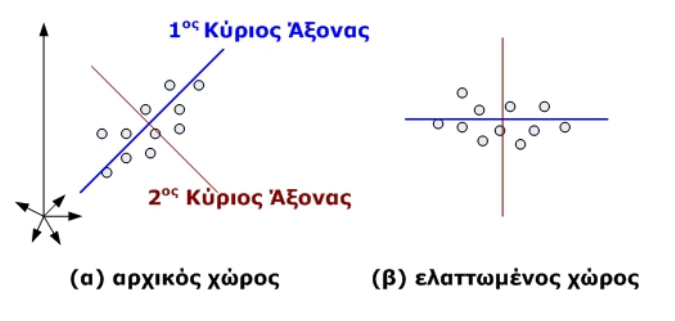
\includegraphics[width=\textwidth,height=20cm,keepaspectratio]{pictures/5.2pca.png} 
\caption{Παράδειγμα λειτουργίας της μεθόδου \en{PCA}}\label{figure5.2}
\end{figure}

\subsection{Η τεχνική \en{SMOTE}}

Για την αντιμετώπιση του προβλήματος της ανισορροπίας των δεδομένων (\en{imbalanced data}), οι ερευνητές Μηχανικής Μάθησης χρησιμοποιούν:
\begin{enumerate}
    \item Είτε τεχνικές \en{oversampling}, οι οποίες έχουν ως στόχο να δημιουργήσουν στιγμιότυπα σε κλάσεις που θεωρούνται μειονότητες σε σχέση με το μέσο όρο
    \item Είτε τεχνικές \en{undersampling} που ακολουθούν την αντίστροφη διαδικασία, αφαιρούν δηλαδή στιγμιότυπα απο τις κλάσεις με το μεγαλύτερο πληθυσμό.
\end{enumerate}

Οι δύο αυτές διαδικασίες χρήζουν ιδιαίτερης προσοχής ώστε, στην πρώτη περίπτωση να μη δημιουργηθούν χαμηλής ποιότητας και αξίας δεδομένα, ή αλλιώς θόρυβος, και στη δεύτερη περίπτωση, να μη χαθεί χρήσιμη πληροφορία. 

Ο αλγόριθμος του \en{SMOTE (Synthetic Minority Oversampling Technique)}, όπως υποδηλώνει και το πλήρες όνομα του, εντοπίζει την κλάση ή τις κλάσεις με τα ελλιπή στιγμιότυπα και συνθέτει νέα στιγμιότυπα από τα ήδη υπάρχοντα, με σκοπό την εξισορρόπηση των στιγμιότυπων μεταξύ των κλάσεων του συνόλου δεδομένων. Τα στιγμιότυπα αυτά είναι συνθετικά και δημιουργούνται αξιοποιώντας τις τιμές των ήδη υπαρχόντων στιγμιοτύπων. 
Εφαρμόζει την προσέγγιση KNN \en{(k-nearest neighbours)}, με βάση τους K πλησιέστερους γείτονες, δημιουργεί τα συνθετικά δείγματα στον χώρο της μειοψηφίας. Ο αλγόριθμος παίρνει τα διανύσματα χαρακτηριστικών από τους πλησιέστερους γείτονές του και υπολογίζει την απόσταση μεταξύ αυτών των διανυσμάτων. Η διαφορά πολλαπλασιάζεται με τυχαίο αριθμό μεταξύ (0, 1) και προστίθεται στο χαρακτηριστικό.

Στο σχήμα ~\ref{figure5.9} γίνεται μια προσπάθεια επεξήγησης του τρόπου λειτουργίας του αλγορίθμου της τεχνικής \en{SMOTE} γραφικά. Τα στιγμιότυπα των κλάσεων με το μεγαλύτερο πληθυσμό απεικονίζονται με μπλε χρώμα, τα στιγμιότυπα των κλάσεων που αποτελούν μειονότητες απεικονίζονται με πράσινο χρώμα και τα συνθετικά στιγμιότυπα που δημιουργεί η τεχνική \en{SMOTE} απεικονίζονται με κόκκινο χρώμα και ενσωματώνονται στην κλάση-μειονότητα:

\begin{figure} [ht!]
\centering
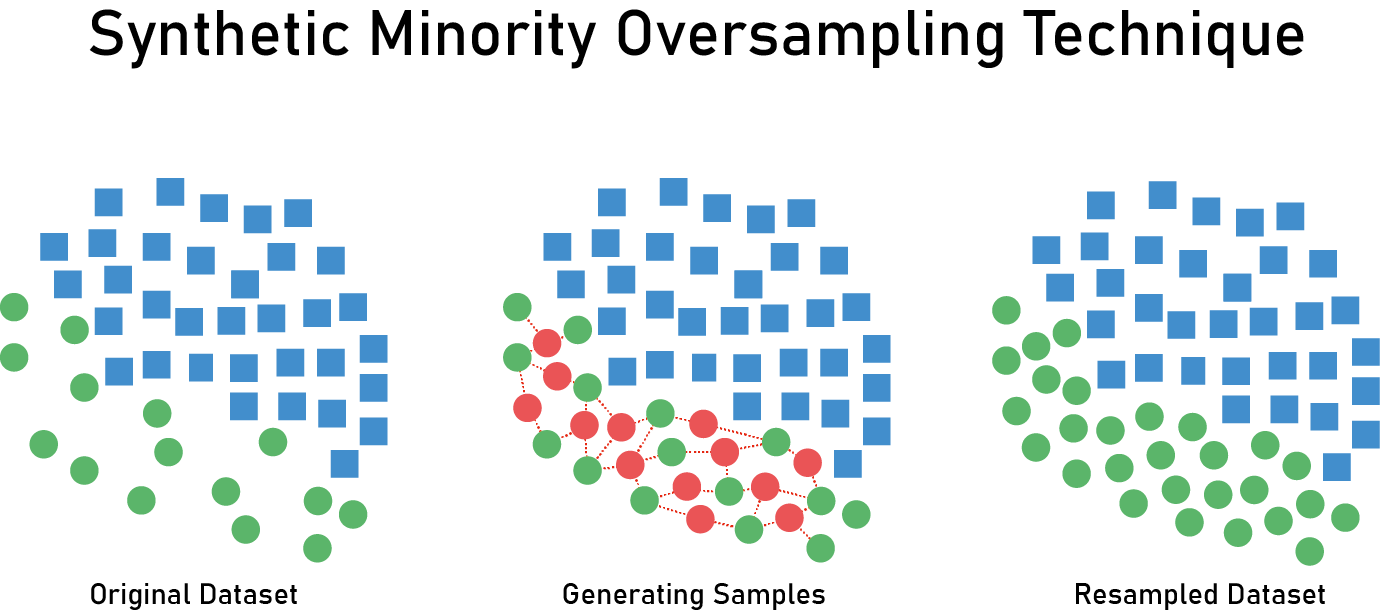
\includegraphics[width=\textwidth,height=12cm,keepaspectratio]{pictures/smote example.png} 
\caption{Γραφική επεξήγηση της λειτουργίας του αλγορίθμου \en{SMOTE}}\label{figure5.9}
\end{figure}


\section{Αλγόριθμοι Ταξινόμησης (\en{Classification Algorithms})}

\subsection{Λογιστική Παλινδρόμηση (\en{Logistic Regression})}
Η Λογιστική Παλινδρόμηση (\en{Logistic Regression}), ή εναλλακτικά το λογιστικό υπόδειγμα πιθανότητας, αποτελεί στην ουσία ένα μη γραμμικό μοντέλο ταξινόμησης των τιμών μιας μεταβλητής απόκρισης Υ με βάση τη θεωρία πιθανοτήτων. Στο λογιστικό μοντέλο το σφάλμα δεν ακολουθεί την κανονική κατανομή. Επίσης, η εξαρτημένη μεταβλητή Υ είναι δυική \en{(boolean)}, δηλαδή παίρνει τιμές 0 και 1 και αναφέρεται στην πραγματοποίηση ή όχι ενός γεγονότος. Η λογιστική παλινδρόμηση χρσηιμοποιείται εκτενώς σε πολλές εφαρμογές όπου επιδιώκεται η πραγματοποίηση πρόβλεψης της παρουσίας ή απουσίας κάποιου χαρακτηριστικού ή γενονότος.
Πρακτικά, αναπτύσσεται μια μη γραμμική συνάρτηση, βάσει της οποίας υπολογίζεται η πιθανότητα ένα στοιχείο να έχει ή όχι το χαρακτηριστικό το οποίο εξετάζεται την κάθε στιγμή. 

Η συνάρτηση αυτή ονομάζεται λογιστική συνάρτηση και εκφράζεται από τον τύπο:

\begin{figure} [ht!]
\centering
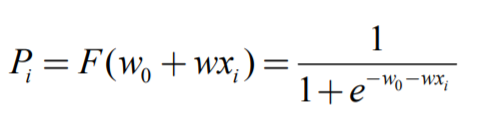
\includegraphics[width=\textwidth,height=2cm,keepaspectratio]{pictures/2logisticR.png} \label{figure2.0}
\end{figure}
\clearpage

Τέλος, αξίζει να σημειωθεί ότι πρώτος ο \en{James A. Ohlson}, το 1980, χρησιμοποίησε το λογιστικό υπόδειγμα πιθανότητας σε έρευνα του σχετικά με την πρόβλεψη της πτώχευσης επιχειρήσεων. \cite{ohlson1980}



%%%%%%%%%%%%%%%%%%   NAIVE BAYES   %%%%%%%%%%%%%%%%%% 

\subsection{\en{Naïve Bayes}}
Ο αλγόριθμος \en{Naïve Bayes} αποτελεί ένα σύνολο πιθανολογικών μοντέλων μηχανικής μάθησης, με σκοπό την επίλυση προβλημάτων ταξινόμησης, το οποίο βασίζεται στο θεώρημα πιθανοτήτων \en{Bayes}.
Αξιοποιώντας το Θεώρημα \en{Bayes} ο αλγόριθμος, για κάθε δεδομένο εισόδου (πχ μήνυμα κειμένου, \en{tweet}, τίτλος άρθρου), προβλέπει, μέσα απο ένα σύνολο δεδομένων διακριτών κατηγοριών, την κατηγορία στην οποία ανήκει. Η πρόβλεψη αποτελεσμάτων από μη επισημασμένα δεδομένα έχει ως προϋπόθεση την ανεξαρτησία μεταξύ των χαρακτηριστικών (\en{features}), μια προϋπόθεση που εάν στην πραγματικότητα αποτελούσε εφικτό στόχο θα απλοποιούσε σημαντικά τη διαδικασία μάθησης.


Ο αλγόριθμος \en{Naïve Bayes} χαρακτηρίζεται ως πιθανολογικός λόγω του ότι η πρόβλεψη γίνεται αποδίδοντας μια πιθανότητα για κάθε δεδομένη κατηγορία και επιστρέφοντας εκείνη με τη μεγαλύτερη πιθανότητα. Οι πιθανότητες υπολογίζονται μεσω του θεωρήματος \en{Bayes}, το οποίο αξιολογεί πιθανολογικά το κάθε χαρακτηριστικό (\en{feature}) ξεχωριστά βάσει της ήδη υπάρχουσας γνώσης που σχετίζεται με αυτό.

\subsubsection{Θεώρημα \en{Bayes}}

\begin{align*}
    P(A/B) = \frac{P(A) * P(B/A)}{P(B)}
\end{align*}
όπου Α και Β γεγονότα.
\begin{itemize}
    \item \en{P(A)} και \en{P(B)} είναι οι πιθανότητες των A και B που είναι ανεξάρτητα μεταξύ τους.
    \item \en{P(A/B),} η υπό συνθήκη πιθανότητα, είναι η πιθανότητα του A δεδομένου του B να είναι αληθής.
    \item \en{P(B/A),} είναι η πιθανότητα του B δεδομένου του A να είναι αληθής.
\end{itemize} \cite{bayesTheorem}
% https://en.wikipedia.org/wiki/Bayes%27_theorem   CITE

To Θεώρημα \en{Bayes} συσχετίζει την τρέχουσα πιθανότητα με την αρχική πιθανότητα. Μπορεί δηλαδή να υπολογιστεί η πιθανότητα να συμβεί ένα γεγονός Α δεδομένου ενός γεγονότος Β. Όταν πρόκειται για πρόβλημα ταξινόμησης το γεγονός Β αναφέρεται στην απόδειξη και το γεγονός Α στην υπόθεση.


\begin{align*}
    P(class/features) = \frac{P(class) * P(features/class)}{P(features)}
\end{align*}

\begin{itemize}
    \item \en{P(class/features)} : εκ των υστέρων πιθανότητα
    \item \en{P(class)} : εκ των προτέρων πιθανότητα κλάσης
    \item \en{P(features/class)} : Δεσμευμένη Πιθανότητα
    \item \en{P(features)} : εκ των υστέρων πιθανότητα ταξινομητή
\end{itemize}


Η \en{P(class/features)} καλείται συνάρτηση πιθανοφάνειας της κλάσης σε σχέση με το χαρακτηριστικό και χρησιμοποιείται για 
να δηλώσει ότι η κατηγορία για την οποία η συνάρτηση έχει μεγάλη τιμή έχει μεγαλύτερη πιθανότητα να  είναι η  σωστή κατηγορία αναφορικά με την πρόβλεψη. Να σημειωθεί ότι το γινόμενο της  πιθανοφάνειας και της εκ των προτέρων πιθανότητας είναι αυτό που  καθορίζει την τιμή της εκ των υστέρων πιθανότητας.

Η βιβλιοθήκη \en{Scikit-learn} της \en{Python} προσφέρει τρεις τύπους μοντέλων  \en{Naïve Bayes}:
\begin{enumerate}
    \item \en{Multinomial Naïve Bayes}: Το συγκεκριμένο μοντέλο χρησιμοποιείται κατα κόρον σε προβλήματα που αφορούν την ταξινόμηση κειμένου σε κατηγορίες που το χαρακτηρίζουν.
    \item \en{Bernoulli Naïve Bayes:} Η διαφοροποίηση του με το \en{Multinomial Naïve Bayes} έγκειται στο οτι οι τιμές πρόβλεψης είναι αυστηρά δυαδικές\en{(boolean)}. Αυτό σημαίνει οτι για κάθε δεδομένο η απάντηση του αλγορίθμου είναι της μορφής ΝΑΙ/ΟΧΙ, κάνοντας το μοντέλο χρήσιμο σε αντίστοιχες εφαρμογές όπως, για παράδειγμα, στην αξιολόγηση ενός κειμένου ως υβριστικού ή όχι.
    \item \en{Gaussian Naïve Bayes:} Στα \en{gaussian} μοντέλα, όπως υποδηλώνει και το όνομα, οι προβλέψεις για κάθε κλάση ακολουθούν την κατανομή \en{Gauss} (Σχήμα ~\ref{figure2.1}). Επομένως οι προβλέψεις εκφράζονται με συνεχείς και όχι διακριτές τιμές. 
\end{enumerate}

\begin{figure}\centering
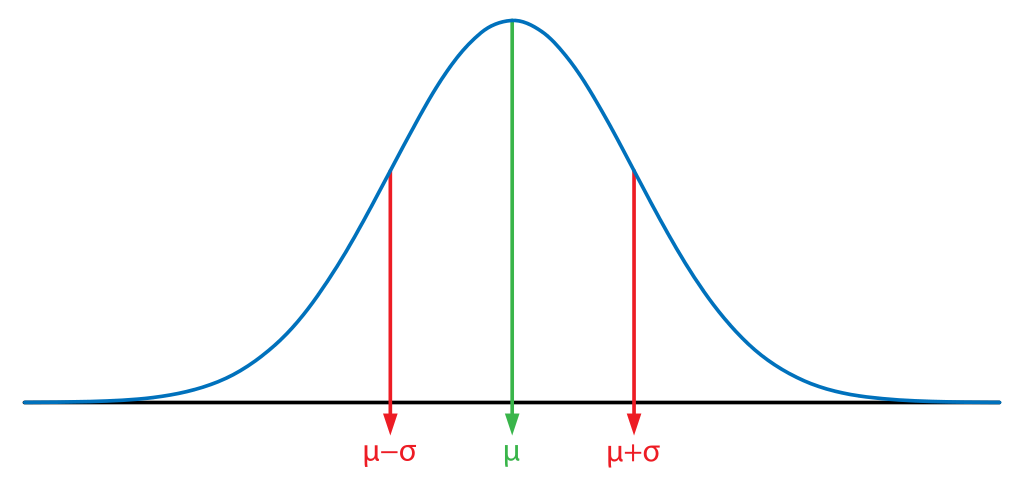
\includegraphics[width=\textwidth,height=14cm,keepaspectratio]{pictures/2.1Gaussian_distribution.png} \caption{Η κατανομή \en{Gauss} (Κανονική κατανομή)}\label{figure2.1}
\end{figure}

\begin{frame}{}
        \hspace{0.5cm} Η συνάρτηση πυκνότητας πιθανότητας της κανονικής κατανομής είναι:
        \begin{equation}
        f(x | \mu,\,\sigma^{2})=\frac{1}{\sqrt{2\,\pi \sigma^{2}}}\,\E^{-\frac{\left(x-\mu\right)^2}{2\,\sigma^2} }
        \end{equation}
        Όπου
        \begin{itemize}
            \item '${\mu}$' είναι η μέση τιμή της μεταβλητής
            \item '${\sigma}$' είναι η τυπική απόκλιση
            \item '${\sigma^2}$' είναι η διακύμανση. 
        \end{itemize}
\end{frame}

%%%%%%%%%%%%%%%%%%   SVM   %%%%%%%%%%%%%%%%%% 

\subsection{\en{Supported Vector Machine}}

Το πρωταρχικό μοντέλο του αλγορίθμου \en{SVM (Supported Vector Machine)} δημιουργήθηκε από τους \en{Vladimir Vapnik} και \en{Alexey Chervonenkis} το 1963. Το 1992, προτάθηκε από τoυς \en{Bernhard Boser, Isabelle Guyon} και \en{Vladimir Vapnik} ένα πιο ισχυρό μοντέλο το οποίο χρησιμοποιείται για την ταξινόμηση δεδομένων σε κατηγορίες και αποτελεί μια τεχνική που χρησιμοποιείται ευρέως στην κατηγοριοποίηση κειμένου λόγω της μεγάλης αποδοτικότητας της. Ο λόγος που θεωρείται ένας απ τους καλύτερους κατηγοριοποιητές στην ταξινόμηση κειμένου είναι η ικανότητα του μοντέλου να διαχειρίζεται μεγάλα σύνολα χαρακτήρων, όπως είναι ένα κείμενο φυσικής γλώσσας.

Ο αλγόριθμος λειτουργεί ως εξής:

Αρχικά παίρνει ως είσοδο το σύνολο δεδομένων εκπαίδευσης (\en{training set}) και δημιουργεί μία απεικόνιση του σε ένα πολυδιάστατο διανυσματικό χώρο. Σε αυτόν το χώρο προσπαθεί να εντοπίσει ένα πεδίο το οποίο να διαχωρίζει τα δύο υποσύνολα δεδομένων, ανάλογα με το αν ανήκουν ή όχι στην εκάστοτε κατηγορία, μεγιστοποιώντας την απόσταση ανάμεσα στο πεδίο και στα δεδομένα εκατέρωθεν του, όπως φαίνεται στο Σχήμα ~\ref{figure2.2}, όπου το διαχωριστικό πεδίο απεικονίζεται με πράσινο χρώμα και ο διαχωρισμός των δύο υποσυνόλων είναι ευδριάκριτος.

Χρησιμοποιώντας έπειτα αυτό το πεδίο, το οποίο ονομάζεται \en{hyperplane.}, ο αλγόριθμος είναι ικανός να προβλέψει αποτελεσματικά την κατηγορία στην οποία ανήκει ένα άγνωστο μέχρι στιγμής δεδομένο εισόδου χαρτογραφώντας το στο χώρο και αποφασίζει σε ποια μεριά του διαχωριστικού πεδίου ανήκει. 

Ο τρόπος του αλγορίθμου να επιλέξει ένα από τα πολλά διαχωριστικά πεδία που θα μπορούσαν να δημιουργηθούν στο διανυσματικό χώρο είναι να επιλέξει το πεδίο με τη μεγαλύτερη απόσταση από τα δεδομένα του εκπαιδευτικού συνόλου, μειώνοντας έτσι τις πιθανότητες σφάλματος στην πρόβλεψη.
\begin{figure}[h!]
\centering
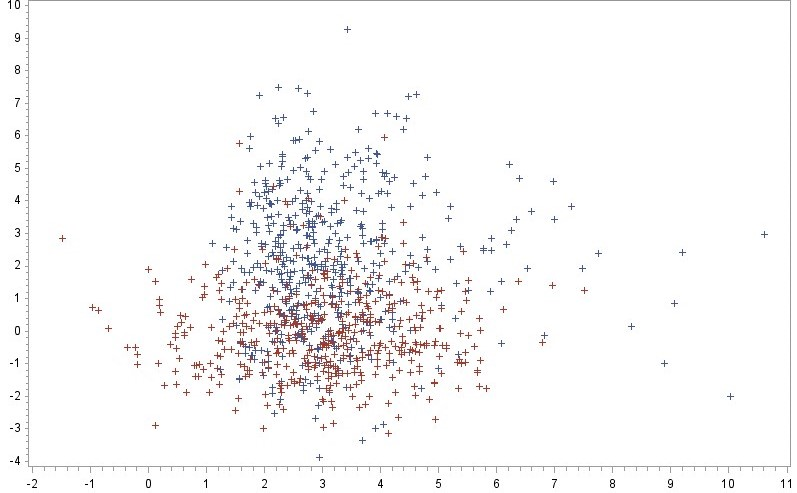
\includegraphics[width=\textwidth,height=10cm,keepaspectratio]{pictures/2.2svmScatter.jpg}
\caption{\en{Scatter Plot:} Παράδειγμα χαρτογράφησης δεδομένων σε χώρο δύο διαστάσεων}
\label{figure2.2}
\end{figure}

\begin{figure}[h!]
\centering
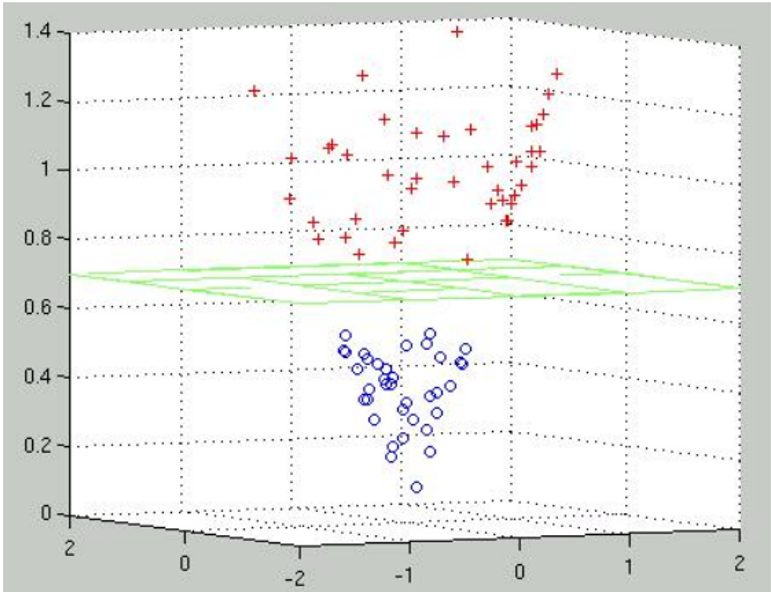
\includegraphics[width=\textwidth,height=10cm,keepaspectratio]{pictures/2.3svm.png}
\caption{Αλγόριθμος \en{SVM:} Παράδειγμα χαρτογράφησης δεδομένων στον πολυδιάστατο διανυσματικό χώρο}
\label{figure2.3}
\end{figure}


\en{\subsection{\en{k Nearest Neighbors - kNN}}

\clearpage
\section{Νευρωνικά Δίκτυα \en{(Neural Networks - NN)}}

Ομοίως με τον άνθρωπο, ένα νευρωνικό δίκτυο απαιτεί εκπαίδευση για να λειτουργήσει σωστά. Η εκπαίδευση περιλαμβάνει τον προσδιορισμό των κατάλληλων συντελεστών βαρών μεταξύ των συνάψεων του, η οποία επιτυγχάνεται μέσω αλγορίθμων που βοηθούν στην εκμάθηση του περιβάλλοντος και τη βελτίωση της απόδοσης του. Η εκπαίδευση ενός νευρωνικού δικτύου είναι μια σταδιακή διαδικασία, η οποία ακολουθεί καθορισμένους κανόνες. Επαναλαμβανόμενες διαδικασίες ρύθμισης των βαρών στις συνάψεις μεταξύ των επιπέδων επιτρέπουν στο νευρωνικό δίκτυο να αποκτήσει περισσότερη "γνώση". Με αυτόν τον τρόπο, το νευρωνικό δίκτυο μπορεί να διπλασιάσει τον όγκο των γνώσεων του, καθιστώντας το πιο αποτελεσματικό στο να ανταποκρίνεται στις απαιτήσεις του περιβάλλοντος στο οποίο επιδρά.





\subsection{\en{Βαθιά Μάθηση (Deep Learning)}}
Η τεχνολογία του deep learning είναι μια προηγμένη μέθοδος μηχανικής μάθησης, η οποία βασίζεται στη χρήση νευρωνικών δικτύων, μια κατηγορία αλγορίθμων με μακρά ιστορία που ξεκινά από τον αλγόριθμο Perceptron του Rosenblatt το 1957 \cite{deep1}  και φτάνει στις σύγχρονες τεχνικές. Στον τομέα της οπτικής αναγνώρισης, οι Geoffrey Hinton και Yann LeCun έχουν κάνει σημαντικές προσπάθειες στην εξέλιξη αυτής της τεχνολογίας.

Αυτά τα δίκτυα είναι σχεδιασμένα να αναλύουν και να εξάγουν χρήσιμες πληροφορίες από μεγάλα σύνολα δεδομένων, σε αντίθεση με τις παραδοσιακές μεθόδους που βασίζονται σε κανόνες και χειροκίνητη επεξεργασία δεδομένων.
Μαθηματικά, τα νευρωνικά δίκτυα είναι μη γραμμικές συναρτήσεις που εκτελούν πολλαπλά επίπεδα επεξεργασίας για την εξαγωγή συμπερασμάτων από τα δεδομένα εισόδου. Η μέθοδος αυτή επιτρέπει στα νευρωνικά δίκτυα να εξάγουν χαρακτηριστικά χωρίς τη χρήση ανθρώπινης παρέμβασης στην επεξεργασία των δεδομένων. Μέσω της επιβλεπόμενης μάθησης, τα νευρωνικά δίκτυα μπορούν να αναγνωρίσουν πρότυπα και σχέσεις στα δεδομένα εισόδου. 

Για παράδειγμα, μπορούν να ταξινομήσουν εικόνες σε διαφορετικές κατηγορίες χρησιμοποιώντας ετικέτες. Σε αυτό το παράδειγμα, η μηχανική μάθηση μπορεί να χρησιμοποιηθεί για να εκπαιδεύσει ένα μοντέλο να αναγνωρίζει εάν μια εικόνα περιέχει ζώο ή άνθρωπο, βασιζόμενο σε ένα σύνολο εκπαίδευσης που περιλαμβάνει εικόνες ταξινομημένες ως απεικόνιση ανθρώπου ή απεικόνιση ζώου. Ενώ για τον ανθρώπινο εγκέφαλο φαντάζει εύκολο να διαχωριστεί η εικόνα ενός ανθρώπου από εκείνη ενός άλλου ζώου, είναι αρκετά δύσκολο να προσδιορίσει κανείς εν είδει μιας ακολουθίας βημάτων (αυτό που στην επιστήμη της πληροφορικής ονομάζεται αλγόριθμος) την διαδικασία που ακολουθεί η λογική σκέψη του για να κάνει αυτήν την ταξινόμηση. 

Το μοντέλο μηχανικής μάθησης μπορεί να εξάγει αυτόματα χαρακτηριστικά από τις εικόνες, όπως γωνίες και συνήθως χρησιμοποιείται ένα νευρωνικό δίκτυο για να εκπαιδευτεί σε αυτά τα χαρακτηριστικά. Στη συνέχεια, το μοντέλο μπορεί να χρησιμοποιηθεί για να ταξινομήσει νέες εικόνες, βασιζόμενο στις παραμέτρους με τις οποίες έχει εκπαιδευτεί.

Η μηχανική μάθηση λοιπόν, χρησιμοποιείται για να δώσει σε έναν υπολογιστή την ικανότητα να αναγνωρίζει πρότυπα και να προβλέπει αποτελέσματα με βάση τα δεδομένα που έχει "δει". Στην ουσία, ο υπολογιστής εκπαιδεύεται με ένα σύνολο δεδομένων εισόδου-εξόδου και μαθαίνει να αναγνωρίζει συσχετίσεις μεταξύ αυτών των δεδομένων, ώστε να μπορεί να κάνει προβλέψεις για νέα δεδομένα.

Το επιθυμητό αποτέλεσμα της επιβλεπόμενης μάθησης επιτυγχάνεται μέσω της βελτιστοποίησης και παραμετροποίησης μιας πολυπαραγοντικής ευέλικτης συνάρτησης, η οποία θα πρέπει να αφομοιώνει και να αναγνωρίζει τις ετικέτες μιας σειράς
ετικετοποιημένων δεδομένων (labelled dataset), γνωστή ως σετ δεδομένων εκπαίδευσης (training dataset). Ο αλγόριθμος αναζητά μέσα στο χώρο όλων των πιθανών τιμών των παραμέτρων με στόχο να προσδιορίσει τη βέλτιστη συνάρτηση η οποία θα ταιριάζει με τα ετικετοποιημένα παραδείγματα με τη μεγαλύτερη δυνατή ακρίβεια. Στη συνέχεια θα χρησιμοποιήσει τη συνάρτηση αυτή για να ταξινομήσει νέες άγνωστες εικόνες που θα δοθούν προς ταξινόμηση.

Ουσιαστικά, τα νευρωνικά δίκτυα είναι τόσο ευέλικτα που μπορούν να προσεγγίσουν μαθηματικά οποιαδήποτε συνάρτηση, χρησιμοποιώντας ένα μεγάλο αριθμό απλών συναρτήσεων που συνδέονται με διάφορους τρόπους. Μπορούν να συνδεθούν σειριακά ή παράλληλα, με τη μία μετασχηματιστική λειτουργία να αποτελεί την είσοδο για την επόμενη ή με πολλές μετασχηματιστικές λειτουργίες να εφαρμόζονται παράλληλα στα δεδομένα και το αποτέλεσμα να συνδυάζεται. Μια από τις βασικές τεχνικές της μηχανικής μάθησης είναι η υπερβολική προσαρμογή (overfitting), όπου το μοντέλο εκπαιδεύεται να ανταποκρίνεται πολύ στα δεδομένα εκπαίδευσης και δεν μπορεί να γενικεύσει σε νέα δεδομένα. Για να αποφευχθεί αυτό, χρησιμοποιούνται τεχνικές όπως η απόσυρση (dropout) και η κανονικοποίηση (regularization).

Αν και ιστορικά η Βαθιά Μάθηση ξεκινά να υπάρχει με την εμφάνιση του αλγόριθμου \en{«perceptron»}, σήμερα χρησιμοποιείται ευρέως ως σύχγρονη τεχνική σε διάφορες εφαρμογές. Η Βαθιά Μάθηση είναι το πεδίο της Μηχανικής Μάθησης που χρησιμοποιεί πιο σύνθετες μορφές μοντέλων, διαχωρισμένων σε πολλά ιεραρχικά επίπεδα. Πιο συγκεκριμένα, αυτά τα μοντέλα ονομάζονται «Βαθιά νευρωνικά δίκτυα», ξεκινούν από ένα επίπεδο δεδομένων εισόδου, το οποίο στη συνέχεια περνά ξεχωριστά από αρκετά «κρυφά» επίπεδα αλλοιώντας κάθε φορά τα χαρακτηριστικά των δεδομένων εισόδου. Με αυτόν τον τρόπο, το μοντέλο αναπτύσσεται ως προς την κατανόηση των δεδομένων εισόδου, με αποτέλεσμα τη σταδιακή βελτίωση του αλγόριθμου ως προς νέα διαθέσιμα δεδομένα. 

Ουσιαστικά, η υπολογιστική μηχανή αποκτά τη δυνατότητα να λειτουργεί με παρόμοιο τρόπο, όπως ο ανθρώπινος εγκέφαλος, να πράττει, δηλαδή, μαθαίντας φυσικά μέσα από παραδείγματα. Με τους αλγόριθμους της Βαθιάς Μάθησης, οι συνδέσεις των δεδομένων γίνονται με τη μορφή «δένδρου» σε πολλαπλά ιεραχικά επίπεδα, γεγονός που θυμίζει τις νευρωνικές συνδέσεις του ανθρώπινου εγκεφάλου, ο οποίος επίσης χρησιμοποιεί απλές υπολογιστικές μονάδες, γνωστές ως νευρώνες, για να πραγματοποιεί πολύπλοκους υπολογισμούς. Ωστόσο, είναι σημαντικό να σημειωθεί ότι τα νευρωνικά δίκτυα δεν αποτελούν ακριβή αντιγραφή του ανθρώπινου εγκεφάλου και οι σύγχρονες επιλογές αρχιτεκτονικών και συναρτήσεων έχουν σχεδιαστεί χωρίς να περιορίζονται στο να αντικατοπτρίζουν πλήρως τον τρόπο λειτουργίας του. \cite{3.5}, \cite{3.9}

\clearpage
\subsection{\en{Μοντέλο Νευρωνικού Δικτύου (Neural Network Model)}}
Ένα νευρωνικό δίκτυο αποτελείται από πολλά μικρά υποσυστήματα που ονομάζονται νευρώνες. Κάθε νευρώνας λαμβάνει είσοδο από άλλους νευρώνες ή από το περιβάλλον και παράγει μια έξοδο, η οποία μπορεί να χρησιμοποιηθεί ως είσοδος σε άλλους νευρώνες.

\begin{figure}[h!]
\centering
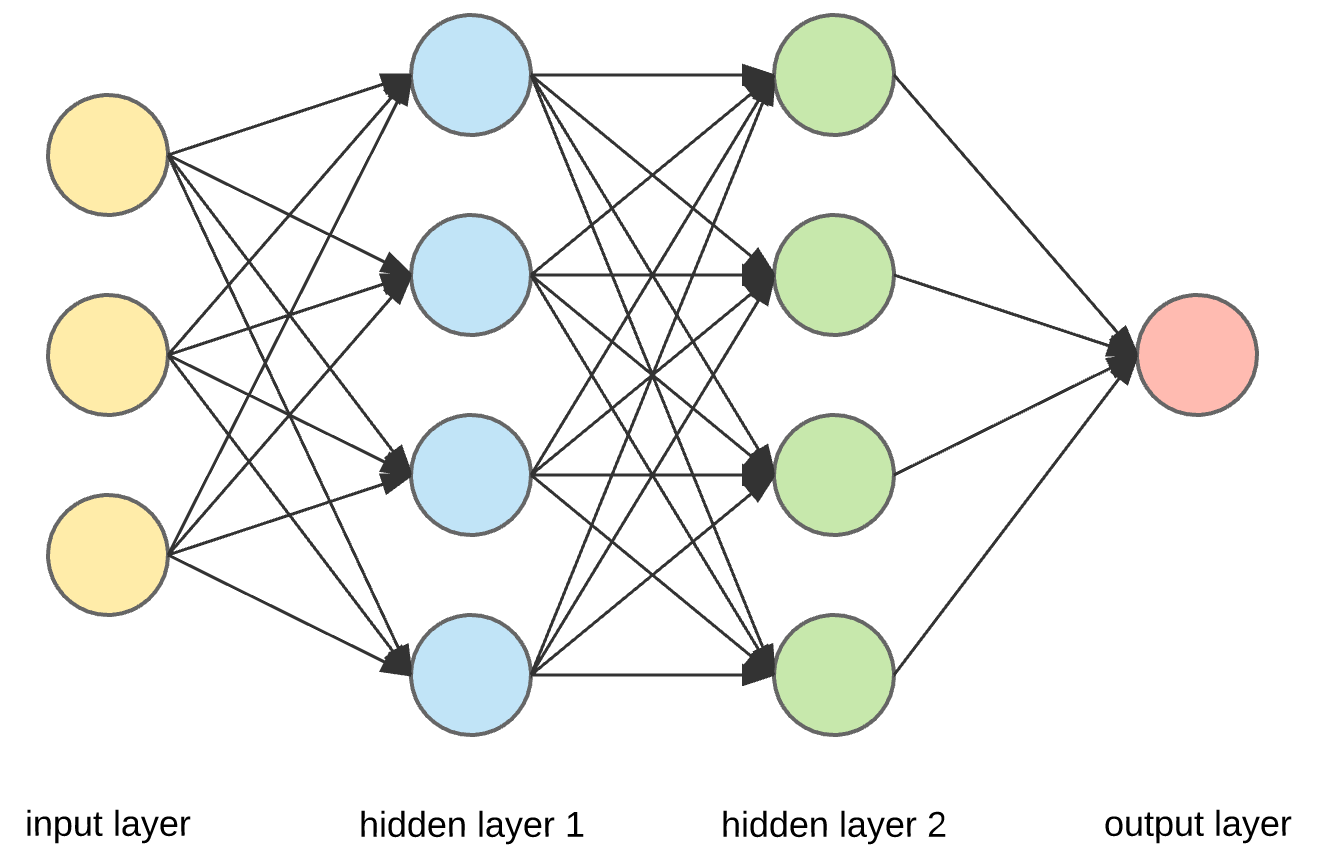
\includegraphics[width=\textwidth,height=10cm,keepaspectratio]{pictures/neural_network.png}
\caption{Απλό μοντέλο νευρωνικού δικτύου που αποτελείται επίπεδα εισόδου, επίπεδα εξόδου και κρυφά επίπεδα.}
\label{figure2.4}
\end{figure}

Κάθε νευρώνας έχει ένα σύνολο βαρών που αντιστοιχεί στις εισόδους του, καθώς και μια συνάρτηση ενεργοποίησης, η οποία καθορίζει το επίπεδο εξόδου που θα παραχθεί, δεδομένων των εισόδων και των σχετικών βαρών.

Τα νευρωνικά δίκτυα είναι οργανωμένα σε επίπεδα (layers), όπου κάθε στρώμα αποτελείται από πολλούς νευρώνες που επεξεργάζονται την ίδια είσοδο. Τα επίπεδα στα νευρωνικά δίκτυα συνήθως χωρίζονται σε τρία είδη: επίπεδο εισόδου (input layer), κρυφό επίπεδο (hidden layer) και επίπεδο εξόδου (output layer).

Το επίπεδο εξόδου αποτελείται από μια ή περισσότερες μονάδες που παράγουν την τελική έξοδο του δικτύου, δηλαδή την πρόβλεψη ή την ταξινόμηση του δεδομένου εισόδου.

Η διαδικασία εκπαίδευσης του νευρωνικού δικτύου συνήθως περιλαμβάνει τη ρύθμιση των βαρών των συνδέσμων μεταξύ των νευρώνων, ώστε να ελαχιστοποιηθεί η απόκλιση της έξοδου του δικτύου από την επιθυμητή έξοδο. Η διαδικασία αυτή γίνεται μέσω της χρήσης ενός αλγορίθμου βελτιστοποίησης, όπως η μέθοδος των ελαχίστων τετραγώνων ή η μέθοδος της ανάδρασης προς τα πίσω (backpropagation).

}


	\chapter{Πρακτικό Μέρος}

\section{\en{Εργαλεία που χρησιμοποιήθηκαν}}
\en{
Η υλοποίηση αυτής της διπλωματικής έγινε χρησιμοποιώντας την γλώσσα προγραμματισμού Python. Παράλληλα, χρησιμοποιήθηκε ένα πολύ ισχυρό εργαλείο για ανάπτυξη κώδικα που ονομάζεται Jupyter Notebook.

Η Python είναι μία από τις πιο δημοφιλείς γλώσσες προγραμματισμού για τον χειρισμό δεδομένων και τον αναλυτικό προγραμματισμό (data analytics). Υπάρχουν διάφοροι λόγοι για αυτό, μερικοί εκ των οποίων είναι:
\begin{itemize}
    \item Είναι εύκολη στην εκμάθηση: Η Python είναι μια ανθρώπινη γλώσσα προγραμματισμού, η οποία σημαίνει ότι είναι σχετικά εύκολο για τους ανθρώπους να την κατανοήσουν. Αυτό την καθιστά ιδανική για χρήση σε επιστημονικά εργαστήρια όπου οι ερευνητές δεν είναι απαραίτητα ειδικοί στον προγραμματισμό.
    \itemΔιαθέτει εκτεταμένη βιβλιοθήκη: Η Python διαθέτει μια εκτεταμένη βιβλιοθήκη που περιλαμβάνει πολλά εργαλεία για τον χειρισμό των δεδομένων. Αυτό σημαίνει ότι οι ερευνητές μπορούν να χρησιμοποιήσουν ένα ευρύ φάσμα εργαλείων και λειτουργιών για την ανάλυση των δεδομένων τους. Αυτά τα πακέτα και βιβλιοθήκες περιλαμβάνουν το NumPy για επιστημονικούς υπολογισμούς, το Pandas για ανάλυση δεδομένων και επεξεργασία, το Matplotlib για οπτικοποίηση δεδομένων, και πολλά άλλα.
    \item H Python είναι μια γλώσσα ανοιχτού κώδικα, η οποία σημαίνει ότι ο κώδικας είναι διαθέσιμος για όλους να τον χρησιμοποιήσουν και να τον βελτιώσουν. Αυτό έχει ως αποτέλεσμα τη δημιουργία μιας πολύ ενεργής και ανοικτής κοινότητας που συνεργάζεται για να δημιουργήσει και να βελτιώσει τις βιβλιοθήκες και τα πακέτα που χρησιμοποιούνται στην ανάλυση δεδομένων.
\end{itemize}


Το Jupyter Notebook είναι μια διαδραστική πλατφόρμα ανάπτυξης λογισμικού, που χρησιμοποιείται για την εκτέλεση κώδικα σε πολλές γλώσσες προγραμματισμού, όπως η Python, η R, η Julia και άλλες. Επιτρέπει στους χρήστες να δημιουργούν και να κοινοποιούν ένα αρχείο σε μορφή notebook που περιέχει κώδικα, αποτελέσματα, εξηγήσεις, εικόνες, γραφήματα και πίνακες.

Τα notebooks αποτελούνται από σελίδες, οι οποίες μπορούν να περιέχουν κελιά κώδικα και κελιά κειμένου. Τα κελιά κώδικα περιέχουν τον κώδικα που εκτελείται σε πραγματικό χρόνο και παράγει τα αποτελέσματα, ενώ τα κελιά κειμένου χρησιμοποιούνται για να παρέχουν εξηγήσεις, οδηγίες ή σχόλια σχετικά με τον κώδικα. Το Jupyter Notebook επιτρέπει στους χρήστες να επεξεργάζονται τα κελιά κώδικα και κειμένου σε πραγματικό χρόνο, επιτρέποντας την αμφίδρομη επικοινωνία με τον κώδικα και τα αποτελέσματα που παράγει.
}


\section{Το \en{dataset}}
Στο κεφάλαιο αυτό αρχικά γίνεται μια περιγραφή το συνόλου δεδομένων \en{(dataset)}  που χρησιμοποιήθηκε για την εκπόνηση της παρούσας εργασίας. 

\subsubsection{Πηγή \en{dataset}}
Το θέμα του ιατρικού απορρήτου καθιστά τη συλλογή και διάθεση ιατρικών δεδομένων δύσκολη διαδικασία. Για το λόγο αυτό, είναι γνωστό στην επιστημονική κοινότητα ότι αποτελούν σπάνια και δύσκολα προσβάσιμη πληροφορία. Το συγκεκριμένο \en{dataset} αντλήθηκε από χρήστες της πλατφόρμας \en{kaggle} \cite{dataset}, με την κύρια πηγή άντλησης να είναι η ιστοσελίδα \en{www.mtsamples.com}. \cite{mtsamples}
Φυσικά, όλες οι εγγραφές είναι απολύτως ανώνυμες. Η πρόκληση του \en{kaggle} είναι η επιτυχής πρόβλεψη της ιατρικής ειδικότητας κάθε περιγραφής ιατρικού περιστατικού.

\subsubsection{Δομή \en{dataset}}
Η αρχική μορφή του \en{dataset} είναι ένα αρχείο \en{csv} με πέντε χιλιάδες (5000) εγγραφές και έξι (6) πεδία και η δομή του έχει ως εξής:
\begin{enumerate}
    \item Α/Α - (Αύξων αριθμός εγγραφής)
    \item \en{description} - (Περιγραφή)
    \item \en{medical specialty} - (Ιατρική ειδικότητα)
    \item \en{sample name} - (Όνομα δείγματος)
    \item \en{transcription} - (Ιατρική συνταγογράφηση)
    \item \en{keywords } - (Λέξεις - κλειδιά)
\end{enumerate}
\clearpage

\begin{figure} [ht!]
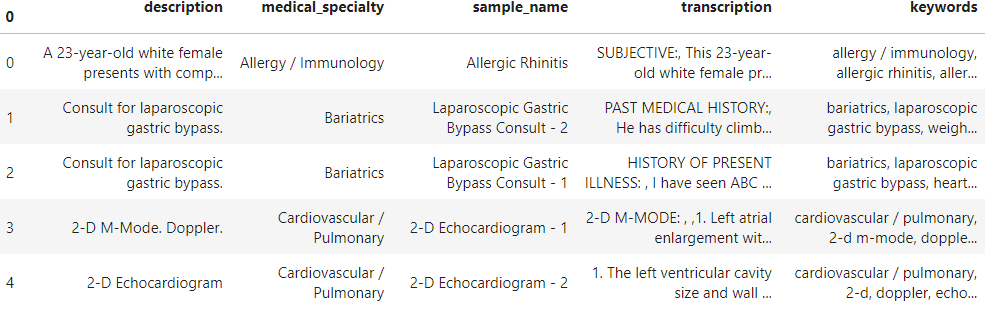
\includegraphics[width=\textwidth,height=\textheight,keepaspectratio]{pictures/3dataset5sthles.png} \caption{Οι πέντε (5) πρώτες στήλες του \en{dataset}}\label{figure3.1}
\end{figure}
Το Σχήμα~ \ref{figure3.1} απεικονίζει ενδεικτικά τις πέντε (5) πρώτες στήλες του \en{dataset} πριν υποστεί οποιαδήποτε επεξεργασία, όπως γίνεται η εισαγωγή του αρχείου \en{csv} στο πρόγραμμα.


Σε πρώτο στάδιο ανάλυσης του συνόλου δεδομένων και με χρήση κατάλληλων εντολών \en{python} εξάγονται πληροφορίες για τον αριθμό των κατηγοριών (Ιατρικών ειδικοτήτων), το όνομα κάθε κατηγορίας καθώς και το πλήθος εγγραφών που περιέχει.

\begin{figure} [ht!]
\centering
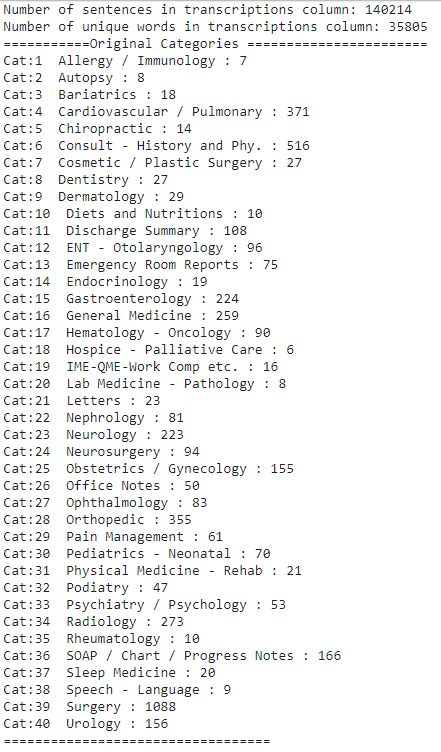
\includegraphics[width=\textwidth,height=20cm,keepaspectratio]{pictures/3categories.png} \caption{Η αρχική κατανομή των δεδομένων στις κατηγορίες}\label{figure3.2}
\end{figure}

Το Σχήμα~ \ref{figure3.2} εμφανίζει τις σαράντα (40) κατηγορίες που περιέχει αρχικά το \en{dataset} καθώς και το πλήθος εγγραφών ανά κατηγορία.

Επίσης, δημιουργείται η συνάρτηση \en{get\_sentence\_word\_count()}, η οποία μας επιστρέφει το πλήθος των διακριτών λέξεων και προτάσεων που υπάρχουν στο πεδίο \en{transcription} του εισαγόμενου αρχείου.
Έτσι έχουμε μια πιο ολοκληρωμένη εικόνα για τη μορφή, τη δομή και την κατανομή των δεδομένων στο αρχείο.

Το επόμενο στάδιο που περιγράφεται στο κεφάλαιο 3 είναι το στάδιο της Προεπεξεργασίας. Η σωστή και καθαρή απεικόνιση των δεδομένων βοηθάει τον ερευνητή να εφαρμόσει πιο στοχευμένες και αποτελεσματικές τεχνικές προεπεξεργασίας κειμένου ώστε να αποφύγει την απώλεια χρήσιμης πληροφορίας. 


\clearpage
\section{Προεπεξεργασία \en{(Preprocessing)}}
Στο κεφάλαιο αυτό  παρουσιάζεται αναλυτικά το στάδιο της Προεπεξεργασίας \en{(Preprocessing)}. Θα παρουσιαστούν εκτενώς όλες οι μέθοδοι και οι τεχνικές που χρησιμοποιήθηκαν, ο σκοπός τους και η τελική μορφή των δεδομένων. 

Είναι σημαντικό να γίνει κατανοητή η σημαντικότητα αυτού του σταδίου για την ακρίβεια των τελικών αποτελεσμάτων. Το αρχικό μας σύνολο δεδομένων περιέχει δύο είδη πληροφορίας. Τη χρήσιμη για τον ερευνητικό σκοπό και όλη την υπόλοιπη η οποία, εάν δεν απομονωθεί σωστά, ενδέχεται να προκαλέσει αλλοίωση των αποτελεσμάτων, εκπαίδευση του συστήματος προς λανθασμένη κατεύθυνση και σίγουρα ανώφελη κατανάλωση υπολογιστικής ισχύος αλλά και χρόνου.

Σε αυτό το στάδιο ο ερευνητής πρέπει να παρατηρήσει σωστά την πληροφορία και να κρατήσει το ωφέλιμο κομμάτι με σκοπό να έχει πιο ποιοτικά δεδομένα, προσέχοντας στην προσπάθεια αυτήν να μην απωλέσει κομμάτι χρήσιμης πληροφορίας που θα εκπαίδευε σωστά το σύστημα.


\subsection{Βήμα 1: Μείωση κατηγοριών και απομόνωση πεδίων}
Είδαμε οτι στο συγκεκριμένο \en{dataset} υπάρχει μεγάλη ανομοιομορφία ως προς την κατανομή των δεδομένων στις διάφορες κατηγορίες. Αυτό αποτελεί ένα μείζον πρόβλημα στους αναλυτές δεδομένων, γνωστό ως \en{Imbalanced Data}, το οποίο οδήγησε την κοινότητα στην ανάπτυξη διάφορων τεχνικών αντιμετώπισης του. Το μεγαλύτερο πρόβλημα έγκειται στο ότι οι αλγόριθμοι ταξινόμησης υποθέτουν οτι όλες οι κλάσεις έχουν ίδο πλήθος δεδομένων και εκπαιδεύονται εξ'ίσου σε όλες.

Επομένως, στο πρώτο βήμα, εξαλείφουμε τις μειονότητες με σκοπό να οδηγηθούμε σε ένα κάπως πιο ισορροπημένο σύνολο δεδομένων. Πρατικά, φιλτράρουμε τα δεδομένα έτσι ώστε να εξαλειφθούν οι κατηγορίες που έχουν λιγότερα απο 50 στοιχεία. 

Εμφανίζουμε ξανά το πλήθος των κατηγοριών και των εγγραφών ανά κατηγορία, καθώς και τη γραφική απεικόνιση σε διάγραμμα μέσω της βιβλιοθήκης \en{matplotlib}. Τα αποτελέσματα φαίνονται στα Σχήματα ~\ref{figure4.1} και ~\ref{figure4.2}
\clearpage

\begin{figure}\centering
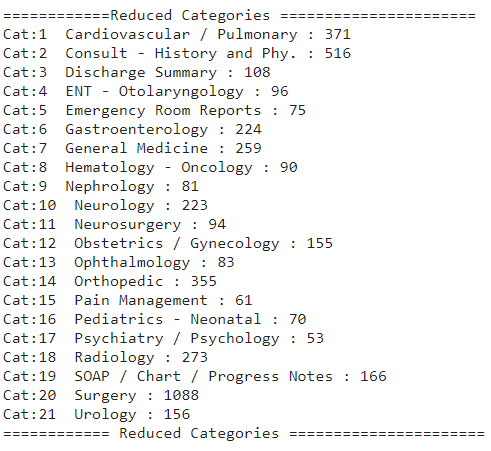
\includegraphics[width=\textwidth,height=9cm,keepaspectratio]{pictures/3reducedCategories.png} \caption{Το πλήθος εγγραφών ανά κατηγορία μετά την εξάλειψη των μειονοτήτων.}\label{figure4.1}
\end{figure}

\begin{figure}\centering
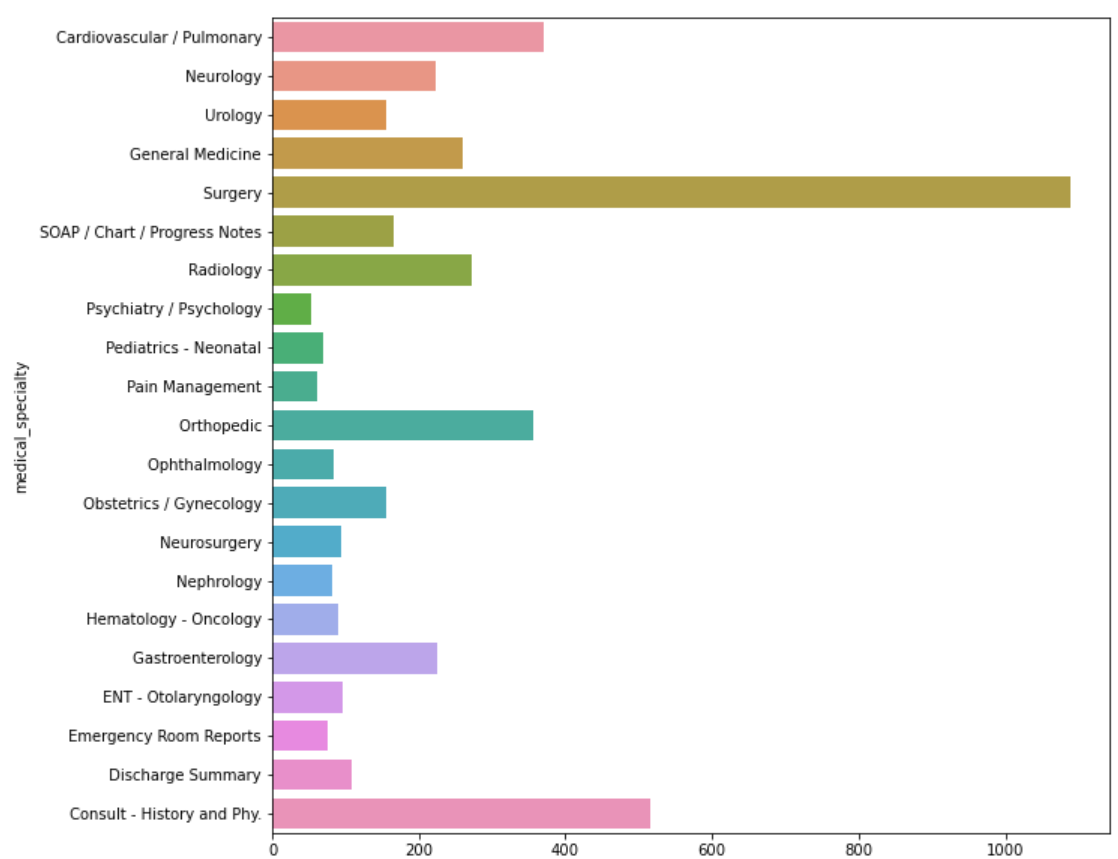
\includegraphics[width=\textwidth,height=14cm,keepaspectratio]{pictures/3categoriesPlot.png} \caption{Γραφικη απεικόνιση του σχήματος 4.1}\label{figure4.2}
\end{figure}
\clearpage
Είδαμε ότι το σύνολο των δεδομένων αποτελείται απο έξι πεδία εκ των οποίων μας αφορούν μόνο δύο:

1) Το πεδίο \en{medical\_specialty} το οποίο αναφέρεται στην κατηγορία/ειδικότητα στην οποία έγκειται το περιστατικό και 

2) Το πεδίο \en{transcription} το οποίο είναι το κυρίως κείμενο και αναφέρεται στην περιγραφή του περιστατικού.  

Επομένως τα δεδομένα φιλτράρoνται ξανά με σκοπό να κρατηθεί μόνο η πληροφορία αυτών των δύο πεδίων και στη συνέχεια αποθηκεύονται σε έναν πίνακα, εμφανίζοντας στο τέλος το πλήθος στηλών και γραμμών. 

Τα δεδομένα πλέον έχουν την εξής μορφή : \en{[4597 rows x 2 columns]}

\subsection{Βήμα 2: Kαθαρισμός κειμένου (\en{text cleaning})}

Στη συνέχεια εκτελείται η διαδικασία καθαρισμού κειμένου (\en{text cleaning process.}) Αρχικά ορίζονται δύο συναρτήσεις: η \en{clean\_text()} και η \en{lemmatize\_text()} οι οποίες επιτελούν τις παρακάτω διεργασίες: 
\begin{enumerate}
    \item Διαίρεση σε όρους \en{(Tokenization)}:
    Με αυτόν τον όρο αναφερόμαστε τον κατακερματισμό μιας συμβολοσειράς σε διακριτές λέξεις. Ο κάθε όρος μπορεί να είναι ολόκληρη λέξη, μεμονομένος χαρακτήρας, αριθμός, σύμβολο ή σημείο στίξης. \cite{lemmatize}. Σε αυτήν την εργασία, η κάθε εγγραφή του πεδίου \en{transcription}, που αποτελούν το κείμενο προς επεξεργασία, χωρίζεται σε λέξεις. Η μορφή των δεδομένων τώρα είναι ένας πίνακας όπου το κείμενο παρουσιάζεται σε μορφή λίστας με διακριτούς όρους.
    
    \item Αφαίρεση λέξεων χωρίς νοηματική αξία \en{stopwords removal}:
    Ένα από τα πιο συνηθισμένα βήματα προεπεξεργασίας κειμένου φυσικής γλώσσας είναι η αφαίρεση λέξεων χωρίς ιδιαίτερη νοηματική αξία. Η βιβλιοθήκη \en{NLTK} της \en{Python} προσφέρει αυτή τη δυνατότητα, απομακρύνοντας λέξεις που δεν αποδίδουν χρήσιμη πληροφορία, αντιθέτως προσθέτουν στο κείμενο θόρυβο και όγκο. Αυτό γίνεται είτε μέσω έτοιμης λίστας \en{stopwords}, είτε εντοπίζοντας λέξεις που εμφανίζονται εξαιρετικά συχνά σε ένα κείμενο. Τέτοιες λέξεις μπορεί να είναι άρθρα, αντωνυμίες, ακόμα και πολύ συνηθισμένα ρήματα.
    
    \item Μετατροπή κεφαλαίων χαρακτήρων σε πεζούς:
    Εδώ γίνεται χρήση της μεθόδου \en{.lower()} που προσφέρει η  \en{python} για μετατροπή συμβολοσειρών, η οποία μετατρέπει οποιοδήποτε κεφαλαίο χαρακτήρα σε πεζό.
    
    \item Απομάκρυνση αριθμών και συμβόλων:
    Οι αριθμοί, τα σύμβολα και τα σημεία στίξης, για το σκοπό της εργασίας, αποτελούν περιττή πληροφορία. Απαλάσσοντας το κείμενο από αυτά μειώνεται ο όγκος εργασίας, η απαιτούμενη υπολογιστική ισχύς και παράγονται πιο ποιοτικά δεδομένα. Έτσι με χρήση κατάλληλων εντολών της \en{python}, όλα αυτά αφαιρούνται.
    
    \item \en{Stemming}
    Ο όρος \en{Stemming} αναφέρεται σε μια διαδικασία που παρέχεται απο τη βιβλιοθήκη \en{NLTK} της \en{Python} η οποία ανάγει όλες τις ομόρριζες λέξεις του κειμένου στην αρχική τους ρίζα, αδιαφορώντας για τις διαφορετικές καταλήξεις που ενδεχομένως να έχουν. Για παράδειγμα, η λέξη \en{coding} ανάγεται στη λέξη \en{code}.
    
    \item Λημματοποίηση \en{(Lemmatization)}
    Ο όρος λημματοποίηση αναφέρεται στη διαδικασία επεξεργασίας κειμένου φυσικής γλώσσας με σκοπό να φέρει την κάθε λέξη σε μια μορφή τέτοια, ώστε να υπάρχει όσο το δυνατόν μικρότερη ποικιλία στο συνολικό λεξιλόγιο, επιδιώκοντας την επιστροφή των λέξεων στο αρχικό τους λήμμα. Η βασική διαφορά των δύο τελευταίων διαδικασιών ειναι οτι στη λημματοποίηση εξετάζεται η γλωσσολογική προέλευση κάθε όρου ώστε να βρεθεί το κατάλληλο λήμμα. Αποτελεί μια πιο εξελιγμένη διαδικασία καθώς το \en{stemming} δεν εξετάζει πληροφορίες που αφορούν τη γλωσσολογική προέλευση της λέξης, αλλά μόνο τη σχέση ρίζας - κατάληξης. Χρησιμοποιώντας και πάλι τη βιβλιοθήκη \en{NLTK} της \en{Python}, γίνεται ομαδοποίηση των λημμάτων μέσω της μεθόδου \en{WordNetLemmatizer()} με βάση το λεξικό \en{WordNet} Για παράδειγμα, στο \en{lemmatization}, η λέξη \en{better} ανάγεται στη λέξη \en{good}.
\end{enumerate}

Σε αυτό το σημείο, η λίστα κειμένων είναι απαλλαγμένη από στοιχεία που προσδίδουν αχρείαστο όγκο, θόρυβο και περιττή πληροφορία. Στα επόμενα κεφάλαια θα χρησιμοποιηθεί το σύνολο δεδομένων με το "καθαρισμένο" κείμενο ως είσοδο στα προγράμματα με σκοπό την εκπαίδευση του συστήματος και την παραγωγή γνώσης.

\clearpage
\section{Υλοποίηση Ταξινόμησης}
Στο προηγούμενο κεφάλαιο φάνηκε αναλυτικά πως τα δεδομένα του \en{dataset} έφτασαν μέσω των διαφόρων διεργασιών της προεπεξεργασίας σε μια πιο ποιοτική και καθαρή μορφή. Για να φανεί χρήσιμη η πληροφορία αυτή, χρειάζεται το αδόμητο κείμενο να μετατραπεί σε κάποια κατανοητή μορφή για τους υπολογιστές, όπως πίνακες ή διανύσματα από χαρακτηριστικά (features).

Αυτό γίνεται με χρήση της μεθόδου \en{tf-idf}, ο τρόπος λειτουργίας της οποίας αναλύθηκε σε προηγούμενο κεφάλαιο. 

Έπειτα, το Σχήμα~ \ref{figure5.1} εμφανίζει την απεικόνιση του πίνακα που προέκυψε από την \en{tf-idf} με χρήση της μεθόδου \en{t-SNE} όπου γίνεται εμφανές πως πολλές κατηγορίες-ειδικότητες αλληλοκαλύπτονται.

\begin{figure} [ht!]
\centering
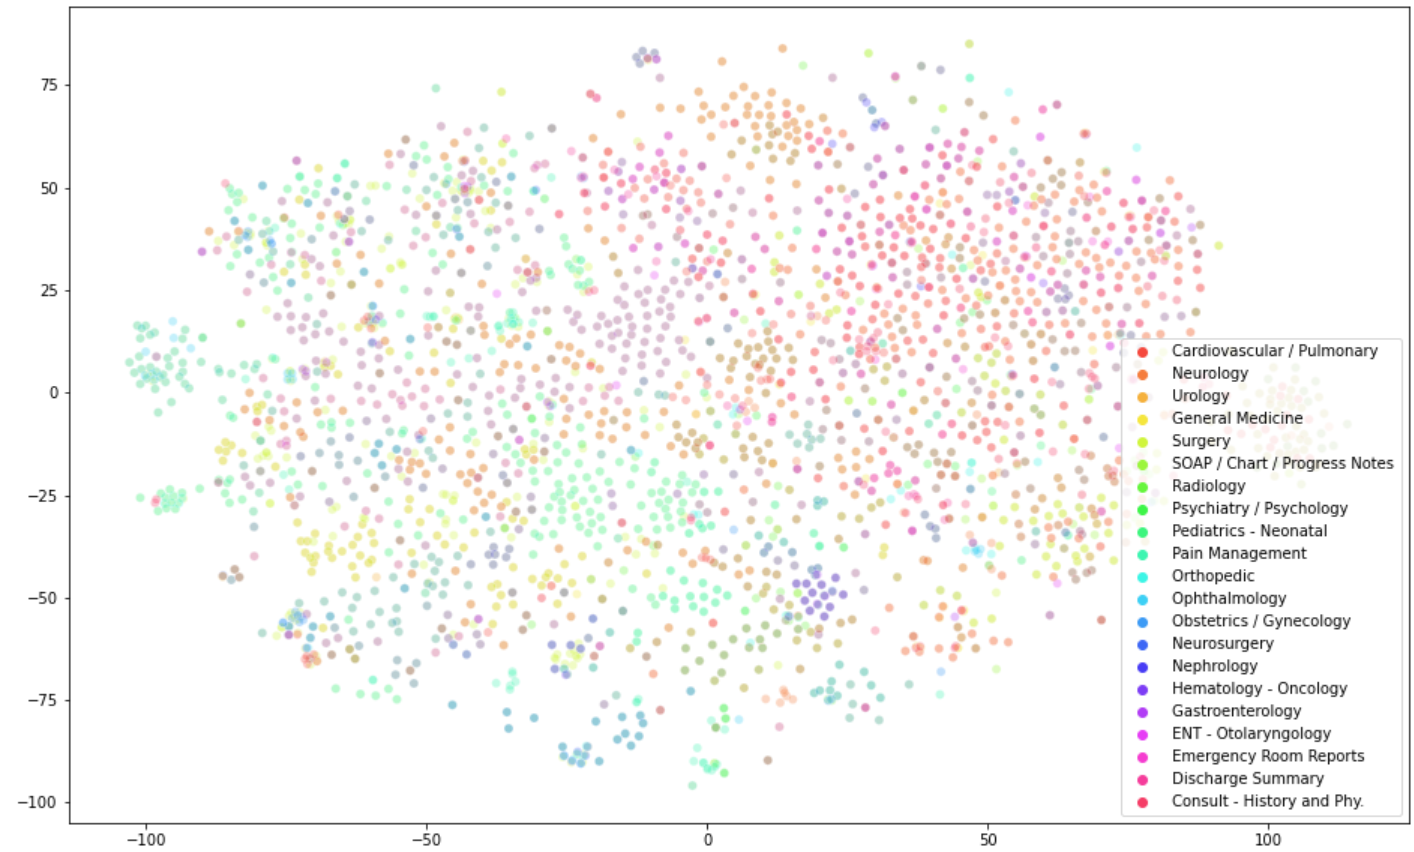
\includegraphics[width=\textwidth,height=20cm,keepaspectratio]{pictures/5.1tsne.png} 
\caption{Η γραφική απεικόνιση του αλγορίθμου \en{t-SNE}}\label{figure5.1}
\end{figure}

Στη συνέχεια εφαρμόζεται η μέθοδος \en{PCA} στον πίνακα \en{tf-idf} με στόχο τη μείωση διαστατικότητας. 

Η \en{Sklearn (ή Scikit-learn)} είναι μια βιβλιοθήκη της \en{Python} η οποία προσφέρει διάφορες δυνατότητες για επεξεργασία δεδομένων και χρησιμοποιείται συνήθως για ταξινόμηση, ομαδοποίηση και επιλογή μοντέλου. 

Για να εκπαιδεύσουμε το μοντέλο χρησιμοποιώντας ένα συγκεκριμένο \en{dataset} θα πρέπει να το «τεστάρουμε» πάνω σε ένα δεύτερο \en{dataset}. Όταν έχουμε μόνο ένα, όπως στη δική μας περίπτωση, το χωρίζουμε στα δύο χρησιμοποιώντας τη μέθοδο \en{train\_test\_split()} της \en{sklearn}. 
Η μέθοδος αυτή χωρίζει το σύνολο των \en{data arrays} σε δύο υποσύνολα: \en{training set} (Σύνολο εκπαίδευσης) και \en{test set} (Σύνολο αξιολόγησης). 

Έτσι, μετά την εφαρμογή του διαχωρισμού έχουμε:
\begin{itemize}
    \item \en{Train\_Set\_Size: (3447, 587) }
    \item \en{Test\_Set\_Size: (1150, 587) }
\end{itemize}


Στη συνέχεια, εφαρμόζουμε στα δεδομένα Λογιστική Παλινδρόμηση \en{(Logistic Regression)} για να εκπαιδεύσουμε το μοντέλο στα \en{training data} και να κάνει την πρόβλεψη στα \en{test data}.
Η εφαρμογή της λογιστικής παλινδρόμησης στη βιβλιοθήκη της \en{Python} \en{scikit-learn} μπορεί να προσεγγιστεί από την κλάση \en{LogisticRegression}. 


Μετά απο αυτήν τη διαδικασία κατασκευάζουμε τον πίνακα σύγχυσης (\en{confusion matrix}). 
Πρόκειται για έναν \en{MxM} πίνακα, όπου το \en{(i,j)} στοιχείο του ισούται με το πλήθος των σημείων που, ενώ προέρχονται από την κλάση \en{i}, καταχωρούνται στην κλάση \en{j}. 
Δίνει πληροφορίες σχετικά με το αν κάποιες κλάσεις έχουν την τάση να συγχέονται με άλλες κλάσεις.

Από τη γραφική απεικόνιση του πίνακα σύγχυσης που φαίνεται στο Σχήμα~ \ref{figure5.3}, παρατηρούμε πως μεγαλύτερη σύγχυση υπάρχει σε συγκεκριμένες ειδικότητες όπως η χειρουργική, οι οποίες έχουν την ιδιότητα υπερκλάσης, αφού επικαλύπτονται με άλλες ειδικότητες εκ φύσεως.

\begin{figure} [ht!]
\centering
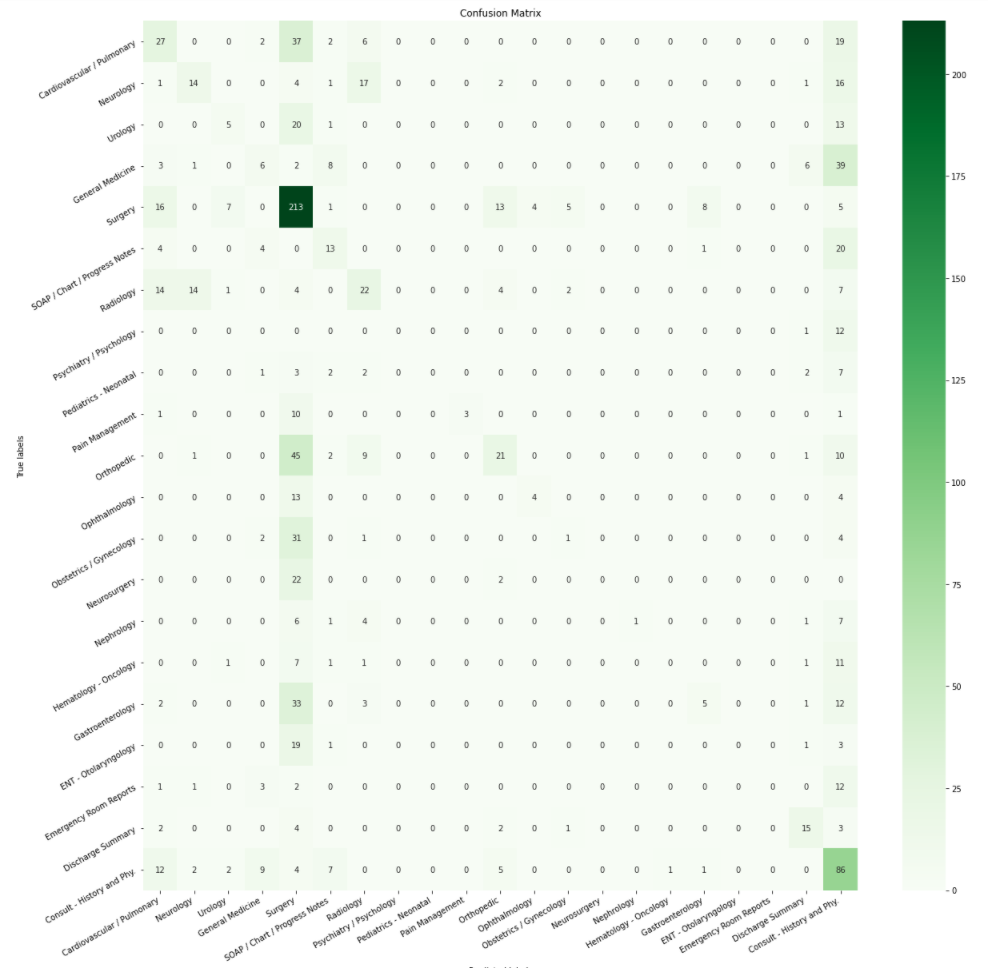
\includegraphics[width=\textwidth,height=20cm,keepaspectratio]{pictures/5.3cMatrix.png} 
\caption{Η γραφική απεικόνιση του πίνακα σύγχυσης}\label{figure5.3}
\end{figure}
\clearpage

H βιβλιοθήκη \en{sklearn} προσφέρει τη μέθοδο \en{classification\_report()} η οποία τυπώνει τις εκτιμήσεις διαφόρων μετρικών πάνω στην ποιότητα  των αποτελεσμάτων πρόβλεψεις του αλγορίθμου. 

Οι μετρικές αυτές είναι:
\begin{enumerate}
    \item Ορθότητα (\en{Accuracy)}
    \item Ανάκληση (\en{Recall)} 
    \item Ακρίβεια (\en{Precision)} 
    \item \en{F-Measure} 
\end{enumerate}

Τα πρώτα αποτελέσματα ακρίβειας ταξινόμησης ανά κατηγορία φαίνονται στον παρακάτω πίνακα (Σχήμα ~\ref{figure5.4}:
 
\begin{figure} [ht!]
\centering
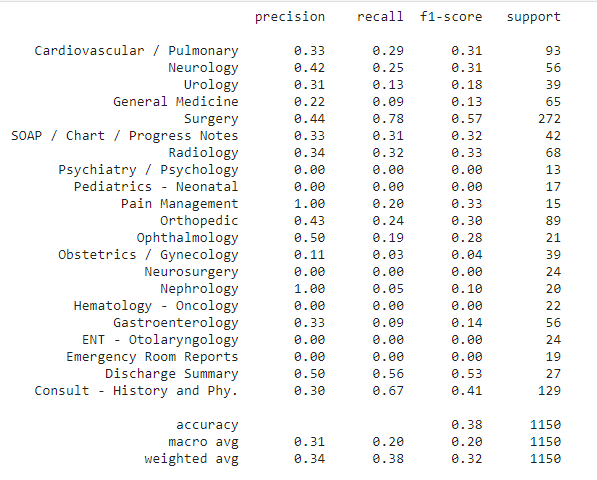
\includegraphics[width=\textwidth,height=20cm,keepaspectratio]{pictures/5.4results.png} 
\caption{Πίνακας πρώτων αποτελεσμάτων μετρικών ταξινόμησης}\label{figure5.4}
\end{figure}
\clearpage

Από το \en{classification report} παρατηρούμε ότι τα αποτελέσματα ακρίβειας είναι αρκετά χαμηλά. Αυτό οφείλεται στο οτι πολλές απο τις κατηγορίες αλληλοεπικαλύπτονται, όπως φαίνεται και στον πίνακα σύγχυσης. Επειδή αυτό συμβαίνει λόγω της φύσης των δεδομένων, καθώς σε κάποια περιστατικά δε γίνεται να αποφανθεί οτι εμπίπτουν μόνο σε μια συγκεκριμένη ιατρική ειδικότητα, στο επόμενο βήμα αφαιρούνται απο το σύνολο των δεδομένων οι ειδικότητες που δημιουργούν αυτόν το «θόρυβο».

Οι ειδικότητες που απαλείφονται είναι: 
\begin{enumerate}
    \en{\item Surgery
        \item SOAP / Chart / Progress Notes
        \item Consult - History and Phy.
        \item Emergency Room Reports
        \item Discharge Summary
        \item Pain Management
        \item General Medicine}
\end{enumerate}


Επίσης, λόγω κοινού γνωστικού πεδίου, συγχωνεύονται οι εξής κατηγορίες:
\begin{enumerate}
    \en{\item Neurosurgery \& Neurology
        \item Nephrology \& Urology}
\end{enumerate}

Ο πίνακας του πλήθους εγγραφών ανα κατηγορία μετά τη διαμόρφωση του έχει τη μορφή που παρουσιάζεται στο Σχήμα ~\ref{figure5.5}:
\begin{figure} [ht!]
\centering
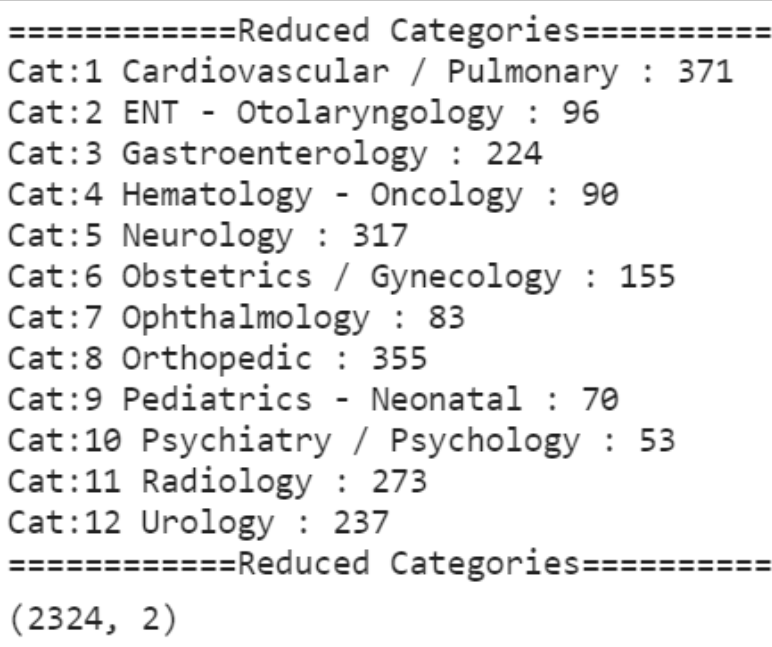
\includegraphics[width=\textwidth,height=7cm,keepaspectratio]{pictures/5.4reducedCat(12cat).png} 
\caption{Το πλήθος εγγραφών ανά κατηγορία μετά την απαλοιφή και τη συγχώνευση κάποιων κατηγοριών}\label{figure5.5}
\end{figure}


Το \en{sciSpacy} είναι ένα πακέτο της  \en{Python} το οποίο περιέχει τα μοντέλα  \en{Spacy} και είναι σχεδιασμένο για προεπεξεργασία σε κείμενα που περιέχουν οντότητες που αποτελούν ιατρική, επιστημονική ή κλινική ορολογία.

Αξιοποιώντας τη δυνατότητα αυτού του πακέτου, δημιουργείται η συνάρτηση \en{process\_text()} η οποία περνάει κάθε εγγραφή του πεδίου \en{transcription} ως είσοδο στη μέθοδο \en{nlp()} του μοντέλου \en{en\_ner\_bionlp13cg\_md} του πακέτου \en{sciSpacy}, η οποία επιστρέφει το σύνολο λέξεων που έχουν ιατρική, επιστημονική ή κλινική νοηματική αξία.


Έπειτα, εφαρμόζουμε αναδρομικά όλη τη διαδικασία:
\begin{enumerate}
    \item Προεπεξεργασία (εφαρμογή \en{sciSpacy})
    \item \en{Tf-Idf} αξιολόγηση
    \item Απεικόνιση του πίνακα \en{Tf-Idf} με χρήση της μεθόδου \en{t-SNE}
    \item Εφαρμογή \en{PCA} στον πίνακα \en{Tf-Idf}
    \item Εκ νέου διαχωρισμός δεδομένων σε \en{training set} και \en{test set}
    \item Εφαρμογή λογιστικής παλινδρόμησης \en{(logistic regression)}
    \item Κατασκευή Πίνακα Σύγχυσης \en{(confusion matrix)}
    \item Εμφάνιση νέων αποτελεσμάτων μετρικών ποιότητας πρόβλεψης
\end{enumerate}

Το Σχήμα~ \ref{figure5.6} εμφανίζει την απεικόνιση του πίνακα που προέκυψε από την \en{tf-idf} με χρήση της μεθόδου \en{t-SNE} μετά την εκ νέου προεπεξεργασία των δεδομένων 

\begin{figure} [ht!]
\centering
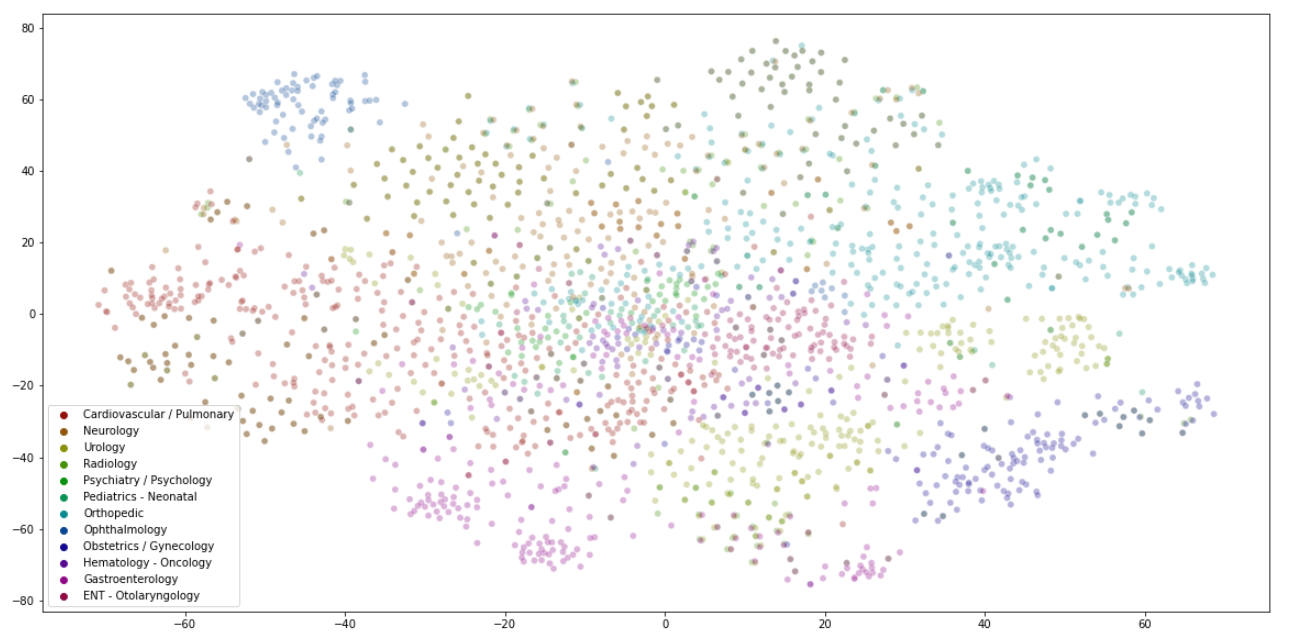
\includegraphics[width=\textwidth,height=12cm,keepaspectratio]{pictures/5.6tsne2.png} 
\caption{Η νέα γραφική απεικόνιση του αλγορίθμου \en{t-SNE}}\label{figure5.6}
\end{figure}


Ο νέος Πίνακας Σύγχυσης και ο νέος Πίνακας αποτελεσμάτων μετρικών ταξινόμησης φαίνονται στα σχήματα ~\ref{figure5.7} και ~\ref{figure5.8}

\begin{figure} [ht!]
\centering
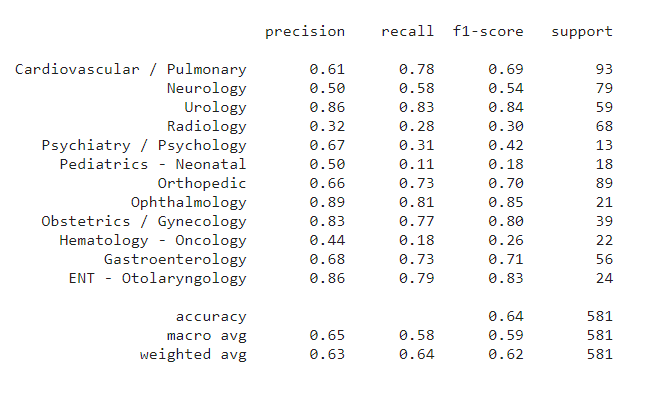
\includegraphics[width=\textwidth,height=8cm,keepaspectratio]{pictures/5.8results2.png} 
\caption{Πίνακας Αποτελεσμάτων μετρικών ταξινόμησης μετά την επεξεργασία με το πακέτο \en{sciSpacy}}\label{figure5.8}
\end{figure}

\begin{figure} [ht!]
\centering
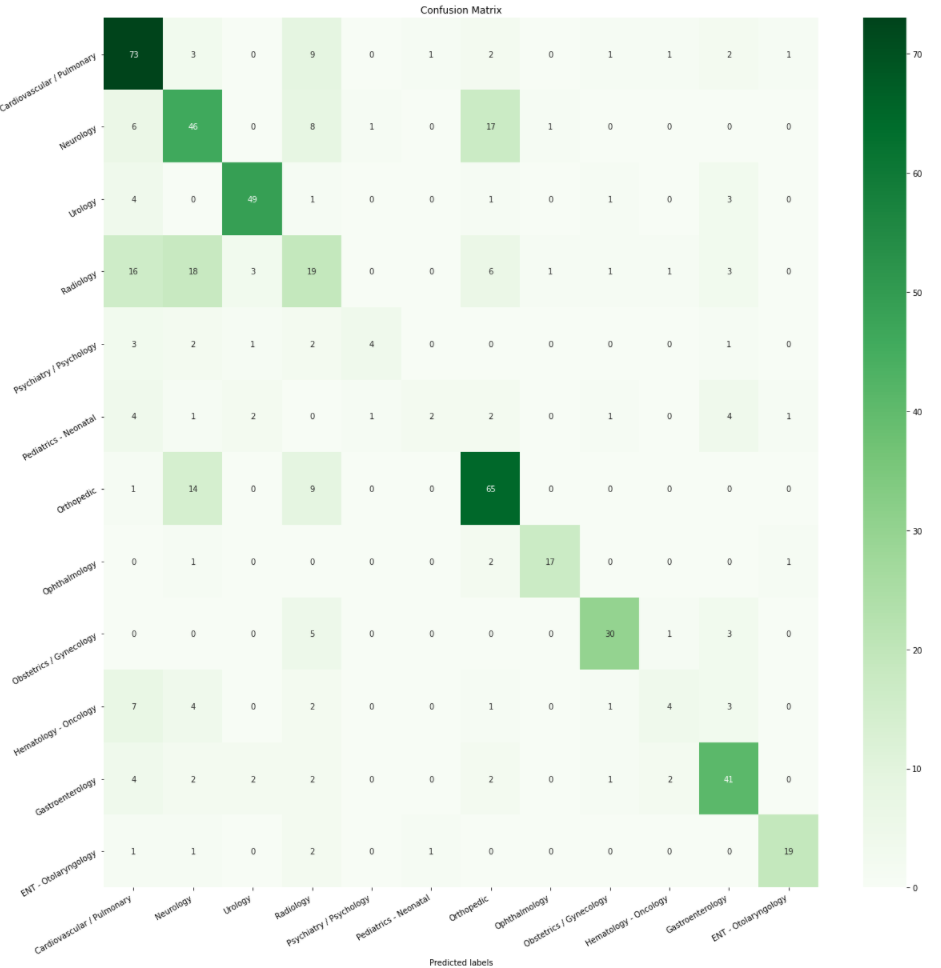
\includegraphics[width=\textwidth,height=12cm,keepaspectratio]{pictures/5.7cMatrix2.png} 
\caption{Πίνακας Σύγχυσης  μετά την επεξεργασία με το πακέτο \en{sciSpacy}}\label{figure5.7}
\end{figure}
\clearpage

Παρατηρούμε εμφανώς βελτιωμένα αποτελέσματα στα \en{scores} των διάφορων μετρικών. (προηγούμενα αποτελέσματα στο σχήμα ~\ref{figure5.4})
Παρ’ όλα αυτά, εξακολουθεί να υπάρχει ανισορροπία στο πλήθος των υπαρχόντων δεδομένων μεταξύ των κατηγοριών. 

Στα πλαίσια της συγκεκριμένης εργασίας ακολουθήθηκαν σε προηγούμενα βήματα και οι δύο προσεγγίσεις αντιμετώπισης της ανισορροπίας των δεδομένων \en{(oversampling} και \en{undersampling}: αφαιρέθηκαν οι κλάσεις που αποτελούσαν μειονότητες καθώς και η κλάση της χειρουρικής που περιείχε δεδομένα κατά πολύ μεγαλύτερα σε όγκο σε σχέση με τις υπόλοιπες κλάσεις τα οποία επίσης συγχέονταν με αυτές λόγω επικαλυπτόμενων γνωστικών πεδίων.

Μία ακόμα απλή προσέγγιση για την αντιμετώπιση του προβλήματος θα ήταν να χρησιμοποιηθεί η απλούστερη \en{oversampling} τεχνική η οποία υποδεικνύει τη δημιουργία διπλότυπων στιγμιοτύπων στις κατηγορίες που αποτελούν μειονότητες. Κάτι τέτοιο όμως, παρ' ότι φαινομενικά επιφέρει μεγαλύτερη ισορροπία στα δεδομένα, δεν προσθέτει καμία καινούρια πληροφορία στο μοντέλο εκπαίδευσης.

Γι' αυτό θα χρησιμοποιηθεί η τεχνική \en{SMOTE (Synthetic Minority Oversampling Technique)}.


Πριν τη δημιουργία νέου \en{dataset} με την τεχνική \en{SMOTE} τα δεδομένα ήταν τα εξής:
\en{
\begin{itemize}
    \item Train\_Set\_Size: (1743, 696)
    \item Test\_Set\_Size: (581, 696) 
\end{itemize}}


Μετά τη δημιουργία νέου \en{dataset} με την τεχνική \en{SMOTE} τα δεδομένα είναι τα εξής:
\en{
\begin{itemize}
    \item Train\_Set\_Size: (1981, 696)
    \item Test\_Set\_Size: (661, 696) 
\end{itemize}
}

\clearpage 
\subsection{Λογιστική Παλινδρόμηση }

Στη συνέχεια γίνεται εφαρμογή Λογιστικής Παλινδρόμησης και παράγεται ο νέος Πίνακας Σύγχυσης (Σχήμα ~ \ref{figure5.10}):

\begin{figure} [ht!]
\centering
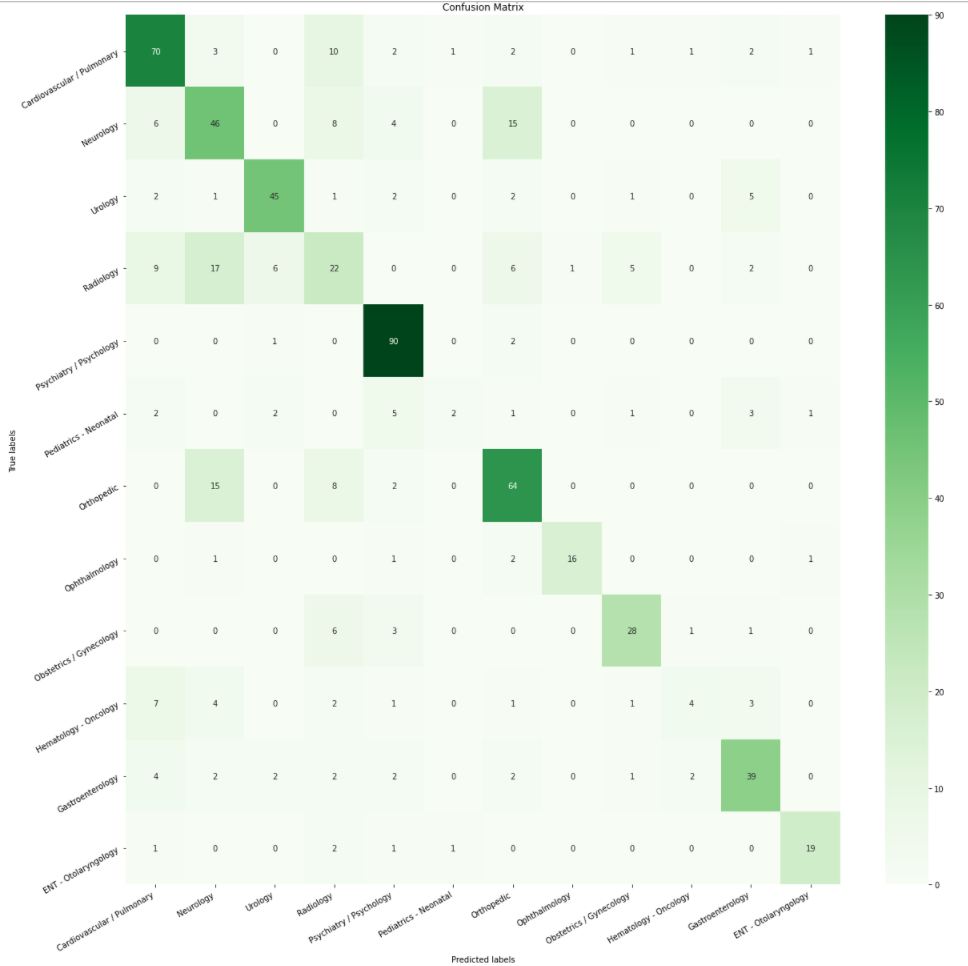
\includegraphics[width=\textwidth,height=12cm,keepaspectratio]{pictures/5.10CMatrix3.png} 
\caption{Πίνακας Σύγχυσης μετά την εφαρμογή της τεχνικής \en{SMOTE}}\label{figure5.10}
\end{figure}

\clearpage
Τέλος, δημιουργείται ο πίνακας των τελικών αποτελεσμάτων μετρικών ταξινόμησης ο οποίος φαίνεται στο σχήμα ~\ref{figure5.11}.

\begin{figure} [ht!]
\centering
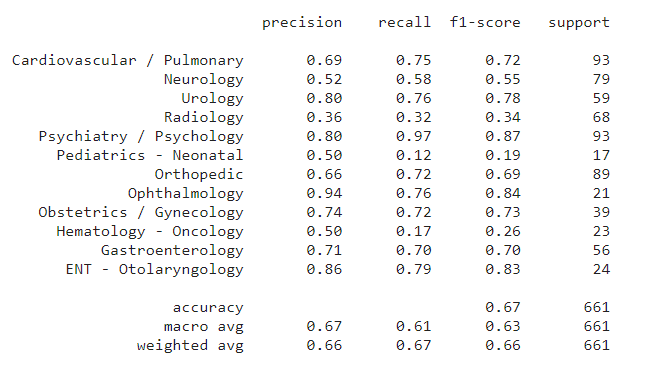
\includegraphics[width=\textwidth,height=8cm,keepaspectratio]{pictures/5.11results3.png} 
\caption{\en{Logistic Regression: }Πίνακας τελικών Αποτελεσμάτων μετρικών ταξινόμησης μετά την εφαρμογή της τεχνικής \en{SMOTE}}\label{figure5.11}
\end{figure}

Τα τελικά αποτελέσματα είναι εμφανώς βελτιωμένα. 
Παρατηρούμε οτι σε συγκεκριμένες κατηγορίες όπως \en{Neurology, Radiology} και \en{Hematology} τα αποτελέσματα ταξινόμησης παραμένουν χαμηλά καθώς οι περιγραφές των περιστατικών εξακολουθούν να αφορούν παραπάνω απο μία ειδικότητες. 


Στη συνέχεια, για την ταξινόμηση του κειμένου, δοκιμάζεται η επίδοση των αλγορίθμων:
\begin{enumerate}
    \item \en{Naïve Bayes} 
    \item \en{SVM}
    \item \en{kNN}
\end{enumerate}


διατηρώντας ως είσοδο το \en{dataset} στην τελευταία μορφή που ταξινομήθηκε με τη μέθοδο της λογιστικής παλινδρόμησης, πριν την επεξεργασία για επίτευξη \en{oversampling} με την τεχνική \en{SMOTE}.

\clearpage
\subsection{Αλγόριθμος \en{Naïve Bayes}}
Ο πίνακας αποτελεσμάτων των μετρικών ταξινόμησης που παράγεται από τη μέθοδο \en{classification\_report()} για τον Αλγόριθμο \en{Naïve Bayes} φαίνεται στο σχήμα ~\ref{figure5.12}.

\begin{figure} [ht!]
\centering
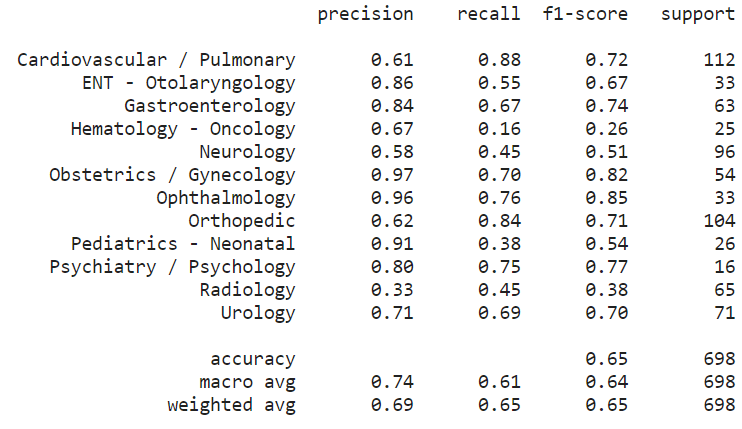
\includegraphics[width=\textwidth,height=8cm,keepaspectratio]{pictures/NAiveBAyes_NO_SMOTE.png} 
\caption{\en{Naïve Bayes: }Πίνακας Αποτελεσμάτων μετρικών ταξινόμησης}\label{figure5.12}
\end{figure}
\clearpage

\subsection{Αλγόριθμος \en{SVM}}

Ο πίνακας αποτελεσμάτων των μετρικών ταξινόμησης που παράγεται από τη μέθοδο \en{classification\_report()} για τον Αλγόριθμο \en{SVM} φαίνεται στο σχήμα ~\ref{figure5.13}.

\begin{figure} [ht!]
\centering
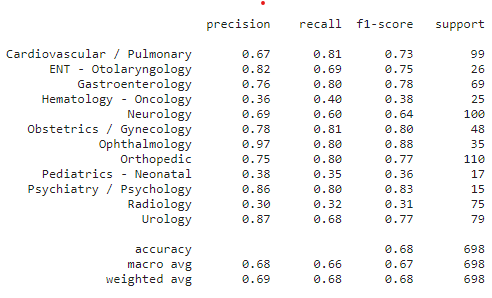
\includegraphics[width=\textwidth,height=8cm,keepaspectratio]{pictures/SVM_NO_SMOTE.png} 
\caption{\en{SVM: }Πίνακας Αποτελεσμάτων μετρικών ταξινόμησης}\label{figure5.13}
\end{figure}
\clearpage

\subsection{Αλγόριθμος \en{kNN}}
Ο πίνακας αποτελεσμάτων των μετρικών ταξινόμησης που παράγεται από τη μέθοδο \en{classification\_report()} για τον Αλγόριθμο \en{kNN} φαίνεται στο σχήμα ~\ref{figure5.14}.

\begin{figure} [ht!]
\centering
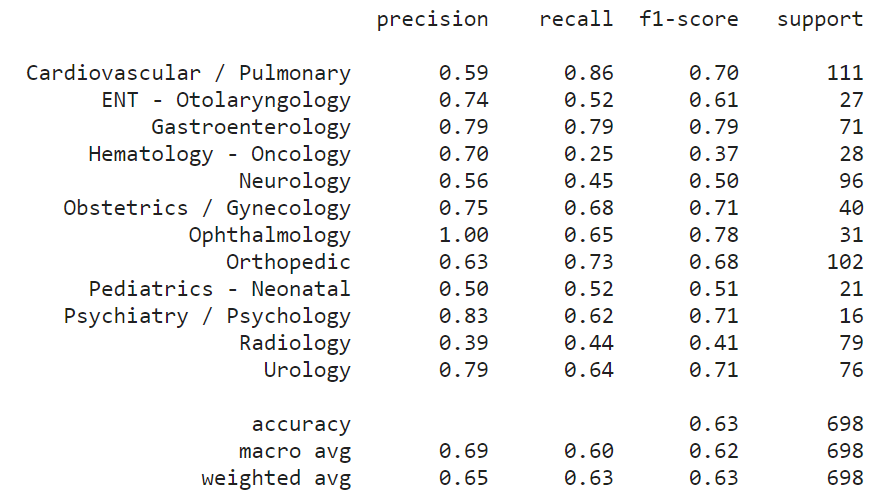
\includegraphics[width=\textwidth,height=8cm,keepaspectratio]{pictures/knn_NO_SMOTE.png} 
\caption{\en{kNN: }Πίνακας Αποτελεσμάτων μετρικών ταξινόμησης}\label{figure5.14}
\end{figure}




\subsection{\en{ΛΕΙΠΕΙ -> Word2Vec - Neural Network}}

\en{\subsubsection{Word Embedding}
Ο όρος Word Embedding είναι ο συλλογικός όρος για τεχνικές μάθησης χαρακτηριστικών όπου οι λέξεις από το λεξιλόγιο αντιστοιχίζονται σε διανύσματα πραγματικών αριθμών. Αυτά τα διανύσματα υπολογίζονται από την πιθανοτική κατανομή για κάθε λέξη που εμφανίζεται πριν ή μετά από μια άλλη. Με άλλα λόγια, λέξεις που εκφράζουν παρόμοιες έννοιες συνήθως εμφανίζονται μαζί στο σώμα κειμένου, επομένως θα είναι κοντά και στον χώρο των διανυσμάτων. 

Στα πλαίσια της παρούσας διπλωματικής, χρησιμοποιείται το πρώτο μοντέλο αυτής της οικογένειας: το Word2Vec της Google (2013). Άλλα δημοφιλή μοντέλα ενσωμάτωσης λέξης είναι το GloVe του Stanford (2014) και το FastText του Facebook (2016).

Το Word2Vec παράγει έναν χώρο διανυσμάτων, συνήθως με εκατοντάδες διαστάσεις, για κάθε διακριτή λέξη του κειμένου, έτσι ώστε οι λέξεις που εκφράζουν παρόμοιες έννοιες να βρίσκονται κοντά η μία στην άλλη στο διανυσματικό χώρο. Αυτό μπορεί να γίνει με δύο διαφορετικές προσεγγίσεις: ξεκινώντας από μια μεμονωμένη λέξη για να προβλέψουμε το συμφραζόμενο της (Skip-gram) ή ξεκινώντας από το συμφραζόμενο για να προβλέψουμε μια λέξη (Continuous Bag-of-Words).

Αρχικά μετατρέπουμε το σύνολο του dataset σε λίστα που περιέχει λίστες (list of lists), κάθε μία εκ των οποίων περιέχει το σύνολο των διακριτών λέξεων του κειμένου μιας εγγραφής.

Κατά την εφαρμογή του Word2Vec, θα πρέπει να καθοριστούν:
\begin{itemize}
    \item Το επιθυμητό μέγεθος των διανυσματικών αναπαραστάσεων των λέξεων. Επιλέχθηκε η τιμή 300.
    \item Το παράθυρο (window), δηλαδή τη μέγιστη απόσταση μεταξύ της τρέχουσας και της προβλεπόμενης λέξης μέσα σε μια πρόταση. Στη συγκεκριμένη υλοποίηση επιλέχθηκε το μέσο μήκος του κειμένου στη συλλογή (TODO: ελεγχος)
    \item Tον αλγόριθμο εκπαίδευσης.  Επιλέχθη η μέθοδος skip-grams (sg=1), καθώς γενικά παρουσιάζει καλύτερα αποτελέσματα.
\end{itemize}

}
	% \chapter{Προεπεξεργασία \en{(Preprocessing)}}
% Στο κεφάλαιο αυτό  παρουσιάζεται αναλυτικά το στάδιο της Προεπεξεργασίας \en{(Preprocessing)}. Θα παρουσιαστούν εκτενώς όλες οι μέθοδοι και οι τεχνικές που χρησιμοποιήθηκαν, ο σκοπός τους και η τελική μορφή των δεδομένων. 

% Είναι σημαντικό να γίνει κατανοητή η σημαντικότητα αυτού του σταδίου για την ακρίβεια των τελικών αποτελεσμάτων. Το αρχικό μας σύνολο δεδομένων περιέχει δύο είδη πληροφορίας. Τη χρήσιμη για τον ερευνητικό σκοπό και όλη την υπόλοιπη η οποία, εάν δεν απομονωθεί σωστά, ενδέχεται να προκαλέσει αλλοίωση των αποτελεσμάτων, εκπαίδευση του συστήματος προς λανθασμένη κατεύθυνση και σίγουρα ανώφελη κατανάλωση υπολογιστικής ισχύος αλλά και χρόνου.

% Σε αυτό το στάδιο ο ερευνητής πρέπει να παρατηρήσει σωστά την πληροφορία και να κρατήσει το ωφέλιμο κομμάτι με σκοπό να έχει πιο ποιοτικά δεδομένα, προσέχοντας στην προσπάθεια αυτήν να μην απωλέσει κομμάτι χρήσιμης πληροφορίας που θα εκπαίδευε σωστά το σύστημα.


% \section{Βήμα 1: Μείωση κατηγοριών και απομόνωση πεδίων}
% Είδαμε οτι στο συγκεκριμένο \en{dataset} υπάρχει μεγάλη ανομοιομορφία ως προς την κατανομή των δεδομένων στις διάφορες κατηγορίες. Αυτό αποτελεί ένα μείζον πρόβλημα στους αναλυτές δεδομένων, γνωστό ως \en{Imbalanced Data}, το οποίο οδήγησε την κοινότητα στην ανάπτυξη διάφορων τεχνικών αντιμετώπισης του. Το μεγαλύτερο πρόβλημα έγκειται στο ότι οι αλγόριθμοι ταξινόμησης υποθέτουν οτι όλες οι κλάσεις έχουν ίδο πλήθος δεδομένων και εκπαιδεύονται εξ'ίσου σε όλες.

% Επομένως, στο πρώτο βήμα, εξαλείφουμε τις μειονότητες με σκοπό να οδηγηθούμε σε ένα κάπως πιο ισορροπημένο σύνολο δεδομένων. Πρατικά, φιλτράρουμε τα δεδομένα έτσι ώστε να εξαλειφθούν οι κατηγορίες που έχουν λιγότερα απο 50 στοιχεία. 

% Εμφανίζουμε ξανά το πλήθος των κατηγοριών και των εγγραφών ανά κατηγορία, καθώς και τη γραφική απεικόνιση σε διάγραμμα μέσω της βιβλιοθήκης \en{matplotlib}. Τα αποτελέσματα φαίνονται στα Σχήματα ~\ref{figure4.1} και ~\ref{figure4.2}
% \clearpage

% \begin{figure}\centering
% 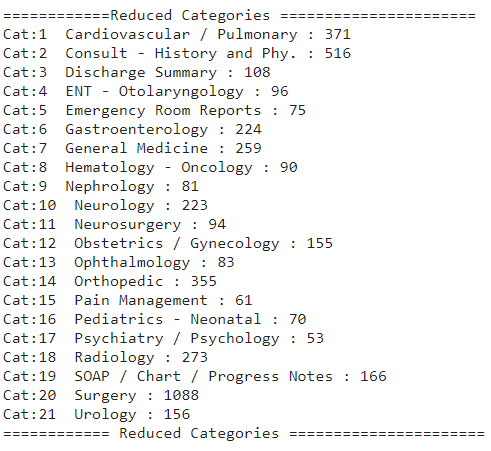
\includegraphics[width=\textwidth,height=9cm,keepaspectratio]{pictures/3reducedCategories.png} \caption{Το πλήθος εγγραφών ανά κατηγορία μετά την εξάλειψη των μειονοτήτων.}\label{figure4.1}
% \end{figure}

% \begin{figure}\centering
% 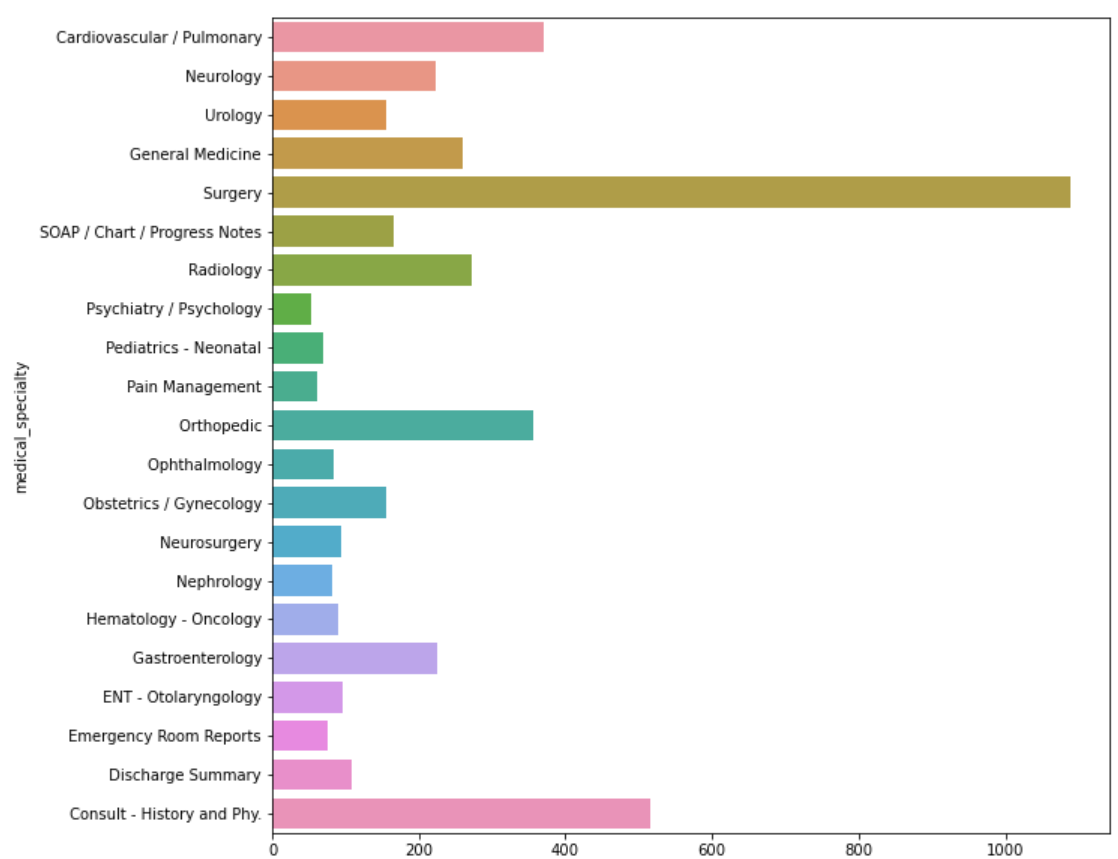
\includegraphics[width=\textwidth,height=14cm,keepaspectratio]{pictures/3categoriesPlot.png} \caption{Γραφικη απεικόνιση του σχήματος 4.1}\label{figure4.2}
% \end{figure}
% \clearpage
% Είδαμε ότι το σύνολο των δεδομένων αποτελείται απο έξι πεδία εκ των οποίων μας αφορούν μόνο δύο:

% 1) Το πεδίο \en{medical\_specialty} το οποίο αναφέρεται στην κατηγορία/ειδικότητα στην οποία έγκειται το περιστατικό και 

% 2) Το πεδίο \en{transcription} το οποίο είναι το κυρίως κείμενο και αναφέρεται στην περιγραφή του περιστατικού.  

% Επομένως τα δεδομένα φιλτράρoνται ξανά με σκοπό να κρατηθεί μόνο η πληροφορία αυτών των δύο πεδίων και στη συνέχεια αποθηκεύονται σε έναν πίνακα, εμφανίζοντας στο τέλος το πλήθος στηλών και γραμμών. 

% Τα δεδομένα πλέον έχουν την εξής μορφή : \en{[4597 rows x 2 columns]}

% \section{Βήμα 2: Kαθαρισμός κειμένου (\en{text cleaning})}

% Στη συνέχεια εκτελείται η διαδικασία καθαρισμού κειμένου (\en{text cleaning process.}) Αρχικά ορίζονται δύο συναρτήσεις: η \en{clean\_text()} και η \en{lemmatize\_text()} οι οποίες επιτελούν τις παρακάτω διεργασίες: 
% \begin{enumerate}
%     \item Διαίρεση σε όρους \en{(Tokenization)}:
%     Με αυτόν τον όρο αναφερόμαστε τον κατακερματισμό μιας συμβολοσειράς σε διακριτές λέξεις. Ο κάθε όρος μπορεί να είναι ολόκληρη λέξη, μεμονομένος χαρακτήρας, αριθμός, σύμβολο ή σημείο στίξης. \cite{lemmatize}. Σε αυτήν την εργασία, η κάθε εγγραφή του πεδίου \en{transcription}, που αποτελούν το κείμενο προς επεξεργασία, χωρίζεται σε λέξεις. Η μορφή των δεδομένων τώρα είναι ένας πίνακας όπου το κείμενο παρουσιάζεται σε μορφή λίστας με διακριτούς όρους.
    
%     \item Αφαίρεση λέξεων χωρίς νοηματική αξία \en{stopwords removal}:
%     Ένα από τα πιο συνηθισμένα βήματα προεπεξεργασίας κειμένου φυσικής γλώσσας είναι η αφαίρεση λέξεων χωρίς ιδιαίτερη νοηματική αξία. Η βιβλιοθήκη \en{NLTK} της \en{Python} προσφέρει αυτή τη δυνατότητα, απομακρύνοντας λέξεις που δεν αποδίδουν χρήσιμη πληροφορία, αντιθέτως προσθέτουν στο κείμενο θόρυβο και όγκο. Αυτό γίνεται είτε μέσω έτοιμης λίστας \en{stopwords}, είτε εντοπίζοντας λέξεις που εμφανίζονται εξαιρετικά συχνά σε ένα κείμενο. Τέτοιες λέξεις μπορεί να είναι άρθρα, αντωνυμίες, ακόμα και πολύ συνηθισμένα ρήματα.
    
%     \item Μετατροπή κεφαλαίων χαρακτήρων σε πεζούς:
%     Εδώ γίνεται χρήση της μεθόδου \en{.lower()} που προσφέρει η  \en{python} για μετατροπή συμβολοσειρών, η οποία μετατρέπει οποιοδήποτε κεφαλαίο χαρακτήρα σε πεζό.
    
%     \item Απομάκρυνση αριθμών και συμβόλων:
%     Οι αριθμοί, τα σύμβολα και τα σημεία στίξης, για το σκοπό της εργασίας, αποτελούν περιττή πληροφορία. Απαλάσσοντας το κείμενο από αυτά μειώνεται ο όγκος εργασίας, η απαιτούμενη υπολογιστική ισχύς και παράγονται πιο ποιοτικά δεδομένα. Έτσι με χρήση κατάλληλων εντολών της \en{python}, όλα αυτά αφαιρούνται.
    
%     \item \en{Stemming}
%     Ο όρος \en{Stemming} αναφέρεται σε μια διαδικασία που παρέχεται απο τη βιβλιοθήκη \en{NLTK} της \en{Python} η οποία ανάγει όλες τις ομόρριζες λέξεις του κειμένου στην αρχική τους ρίζα, αδιαφορώντας για τις διαφορετικές καταλήξεις που ενδεχομένως να έχουν. Για παράδειγμα, η λέξη \en{coding} ανάγεται στη λέξη \en{code}.
    
%     \item Λημματοποίηση \en{(Lemmatization)}
%     Ο όρος λημματοποίηση αναφέρεται στη διαδικασία επεξεργασίας κειμένου φυσικής γλώσσας με σκοπό να φέρει την κάθε λέξη σε μια μορφή τέτοια, ώστε να υπάρχει όσο το δυνατόν μικρότερη ποικιλία στο συνολικό λεξιλόγιο, επιδιώκοντας την επιστροφή των λέξεων στο αρχικό τους λήμμα. Η βασική διαφορά των δύο τελευταίων διαδικασιών ειναι οτι στη λημματοποίηση εξετάζεται η γλωσσολογική προέλευση κάθε όρου ώστε να βρεθεί το κατάλληλο λήμμα. Αποτελεί μια πιο εξελιγμένη διαδικασία καθώς το \en{stemming} δεν εξετάζει πληροφορίες που αφορούν τη γλωσσολογική προέλευση της λέξης, αλλά μόνο τη σχέση ρίζας - κατάληξης. Χρησιμοποιώντας και πάλι τη βιβλιοθήκη \en{NLTK} της \en{Python}, γίνεται ομαδοποίηση των λημμάτων μέσω της μεθόδου \en{WordNetLemmatizer()} με βάση το λεξικό \en{WordNet} Για παράδειγμα, στο \en{lemmatization}, η λέξη \en{better} ανάγεται στη λέξη \en{good}.
% \end{enumerate}

% Σε αυτό το σημείο, η λίστα κειμένων είναι απαλλαγμένη από στοιχεία που προσδίδουν αχρείαστο όγκο, θόρυβο και περιττή πληροφορία. Στα επόμενα κεφάλαια θα χρησιμοποιηθεί το σύνολο δεδομένων με το "καθαρισμένο" κείμενο ως είσοδο στα προγράμματα με σκοπό την εκπαίδευση του συστήματος και την παραγωγή γνώσης.
	% \chapter{Υλοποίηση}
% Στο προηγούμενο κεφάλαιο φάνηκε αναλυτικά πως τα δεδομένα του \en{dataset} έφτασαν μέσω των διαφόρων διεργασιών της προεπεξεργασίας σε μια πιο ποιοτική και καθαρή μορφή. Για να φανεί χρήσιμη η πληροφορία αυτή, χρειάζεται το αδόμητο κείμενο να μετατραπεί σε κάποια κατανοητή μορφή για τους υπολογιστές, όπως πίνακες ή διανύσματα από χαρακτηριστικά (features).

% Αυτό γίνεται με χρήση της μεθόδου \en{tf-idf}, ο τρόπος λειτουργίας της οποίας αναλύθηκε σε προηγούμενο κεφάλαιο. 

% Έπειτα, το Σχήμα~ \ref{figure5.1} εμφανίζει την απεικόνιση του πίνακα που προέκυψε από την \en{tf-idf} με χρήση της μεθόδου \en{t-SNE} όπου γίνεται εμφανές πως πολλές κατηγορίες-ειδικότητες αλληλοκαλύπτονται.

% \begin{figure} [ht!]
% \centering
% 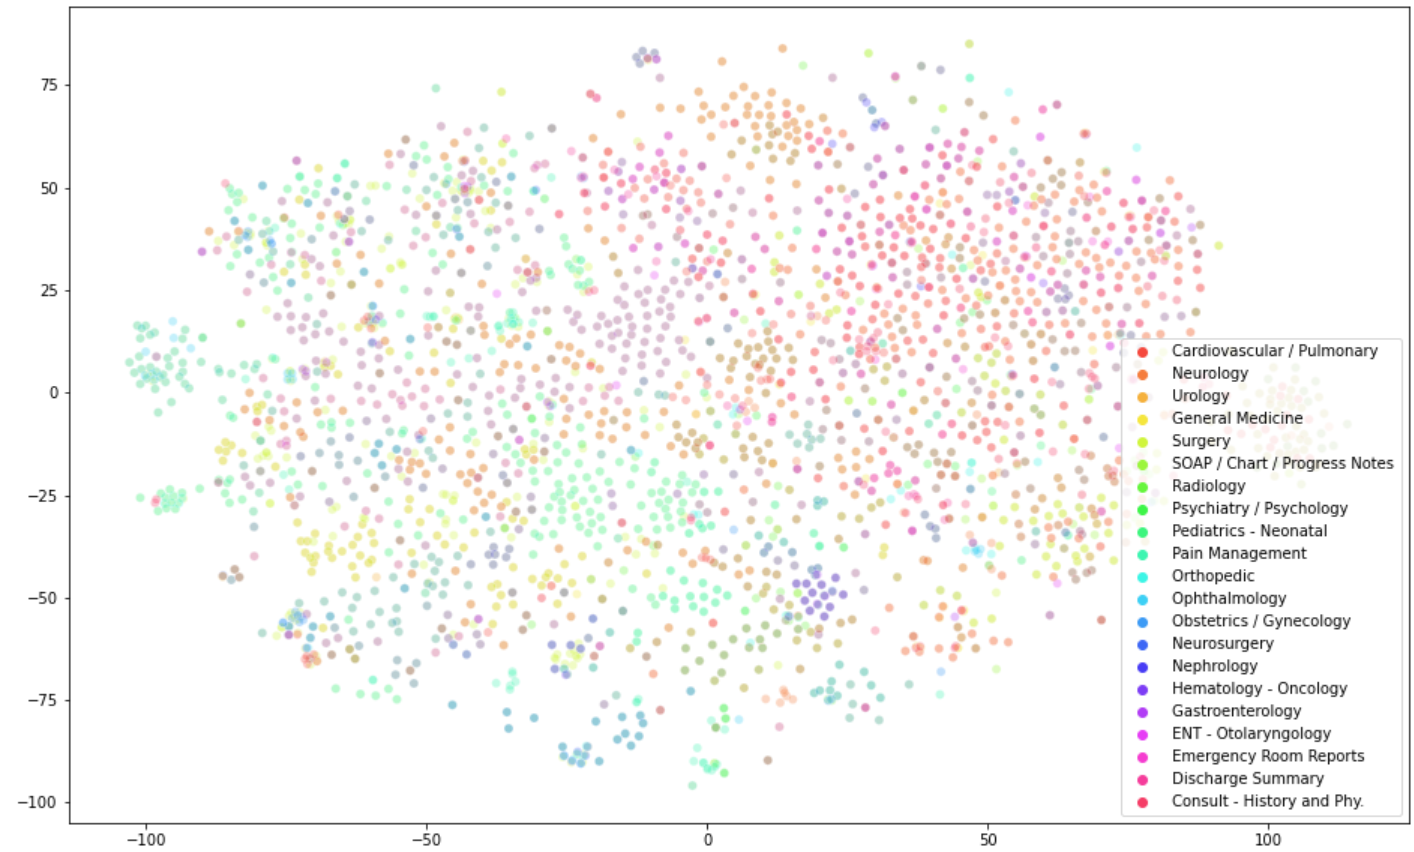
\includegraphics[width=\textwidth,height=20cm,keepaspectratio]{pictures/5.1tsne.png} 
% \caption{Η γραφική απεικόνιση του αλγορίθμου \en{t-SNE}}\label{figure5.1}
% \end{figure}

% Στη συνέχεια εφαρμόζεται η μέθοδος \en{PCA} στον πίνακα \en{tf-idf} με στόχο τη μείωση διαστατικότητας. 

% Η \en{Sklearn (ή Scikit-learn)} είναι μια βιβλιοθήκη της \en{Python} η οποία προσφέρει διάφορες δυνατότητες για επεξεργασία δεδομένων και χρησιμοποιείται συνήθως για ταξινόμηση, ομαδοποίηση και επιλογή μοντέλου. 

% Για να εκπαιδεύσουμε το μοντέλο χρησιμοποιώντας ένα συγκεκριμένο \en{dataset} θα πρέπει να το «τεστάρουμε» πάνω σε ένα δεύτερο \en{dataset}. Όταν έχουμε μόνο ένα, όπως στη δική μας περίπτωση, το χωρίζουμε στα δύο χρησιμοποιώντας τη μέθοδο \en{train\_test\_split()} της \en{sklearn}. 
% Η μέθοδος αυτή χωρίζει το σύνολο των \en{data arrays} σε δύο υποσύνολα: \en{training set} (Σύνολο εκπαίδευσης) και \en{test set} (Σύνολο αξιολόγησης). 

% Έτσι, μετά την εφαρμογή του διαχωρισμού έχουμε:
% \begin{itemize}
%     \item \en{Train\_Set\_Size: (3447, 587) }
%     \item \en{Test\_Set\_Size: (1150, 587) }
% \end{itemize}


% Στη συνέχεια, εφαρμόζουμε στα δεδομένα Λογιστική Παλινδρόμηση \en{(Logistic Regression)} για να εκπαιδεύσουμε το μοντέλο στα \en{training data} και να κάνει την πρόβλεψη στα \en{test data}.
% Η εφαρμογή της λογιστικής παλινδρόμησης στη βιβλιοθήκη της \en{Python} \en{scikit-learn} μπορεί να προσεγγιστεί από την κλάση \en{LogisticRegression}. 


% Μετά απο αυτήν τη διαδικασία κατασκευάζουμε τον πίνακα σύγχυσης (\en{confusion matrix}). 
% Πρόκειται για έναν \en{MxM} πίνακα, όπου το \en{(i,j)} στοιχείο του ισούται με το πλήθος των σημείων που, ενώ προέρχονται από την κλάση \en{i}, καταχωρούνται στην κλάση \en{j}. 
% Δίνει πληροφορίες σχετικά με το αν κάποιες κλάσεις έχουν την τάση να συγχέονται με άλλες κλάσεις.

% Από τη γραφική απεικόνιση του πίνακα σύγχυσης που φαίνεται στο Σχήμα~ \ref{figure5.3}, παρατηρούμε πως μεγαλύτερη σύγχυση υπάρχει σε συγκεκριμένες ειδικότητες όπως η χειρουργική, οι οποίες έχουν την ιδιότητα υπερκλάσης, αφού επικαλύπτονται με άλλες ειδικότητες εκ φύσεως.

% \begin{figure} [ht!]
% \centering
% 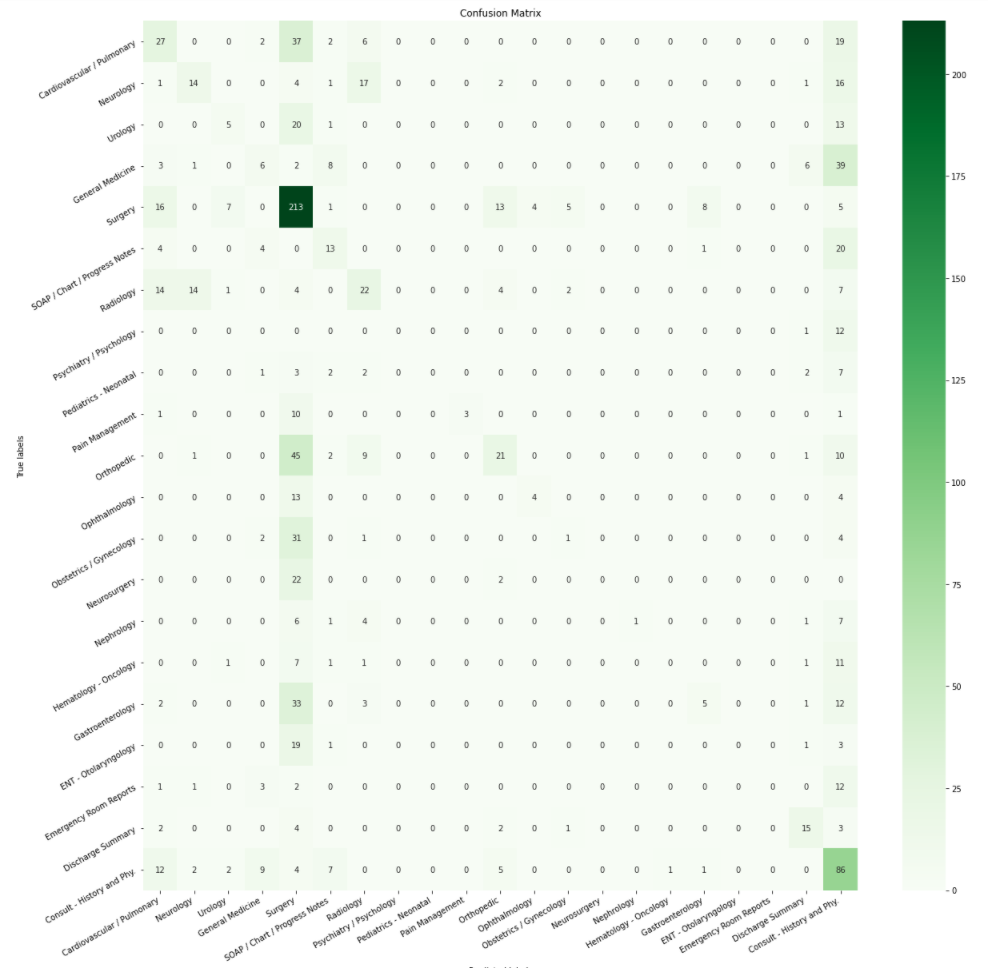
\includegraphics[width=\textwidth,height=20cm,keepaspectratio]{pictures/5.3cMatrix.png} 
% \caption{Η γραφική απεικόνιση του πίνακα σύγχυσης}\label{figure5.3}
% \end{figure}
% \clearpage

% H βιβλιοθήκη \en{sklearn} προσφέρει τη μέθοδο \en{classification\_report()} η οποία τυπώνει τις εκτιμήσεις διαφόρων μετρικών πάνω στην ποιότητα  των αποτελεσμάτων πρόβλεψεις του αλγορίθμου. 

% Οι μετρικές αυτές είναι:
% \begin{enumerate}
%     \item Ορθότητα (\en{Accuracy)}
%     \item Ανάκληση (\en{Recall)} 
%     \item Ακρίβεια (\en{Precision)} 
%     \item \en{F-Measure} 
% \end{enumerate}

% Τα πρώτα αποτελέσματα ακρίβειας ταξινόμησης ανά κατηγορία φαίνονται στον παρακάτω πίνακα (Σχήμα ~\ref{figure5.4}:
 
% \begin{figure} [ht!]
% \centering
% 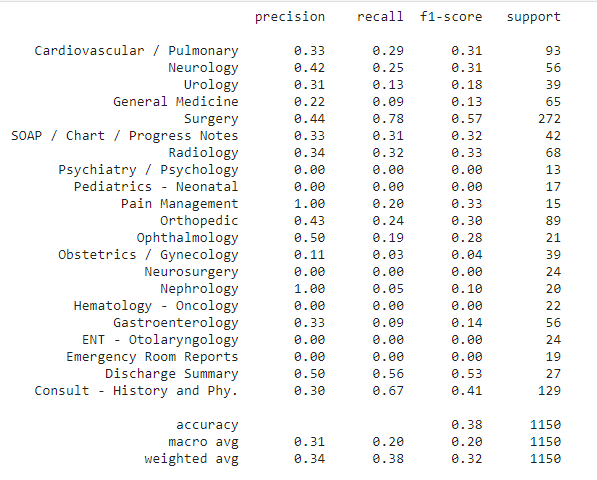
\includegraphics[width=\textwidth,height=20cm,keepaspectratio]{pictures/5.4results.png} 
% \caption{Πίνακας πρώτων αποτελεσμάτων μετρικών ταξινόμησης}\label{figure5.4}
% \end{figure}
% \clearpage

% Από το \en{classification report} παρατηρούμε ότι τα αποτελέσματα ακρίβειας είναι αρκετά χαμηλά. Αυτό οφείλεται στο οτι πολλές απο τις κατηγορίες αλληλοεπικαλύπτονται, όπως φαίνεται και στον πίνακα σύγχυσης. Επειδή αυτό συμβαίνει λόγω της φύσης των δεδομένων, καθώς σε κάποια περιστατικά δε γίνεται να αποφανθεί οτι εμπίπτουν μόνο σε μια συγκεκριμένη ιατρική ειδικότητα, στο επόμενο βήμα αφαιρούνται απο το σύνολο των δεδομένων οι ειδικότητες που δημιουργούν αυτόν το «θόρυβο».

% Οι ειδικότητες που απαλείφονται είναι: 
% \begin{enumerate}
%     \en{\item Surgery
%         \item SOAP / Chart / Progress Notes
%         \item Consult - History and Phy.
%         \item Emergency Room Reports
%         \item Discharge Summary
%         \item Pain Management
%         \item General Medicine}
% \end{enumerate}


% Επίσης, λόγω κοινού γνωστικού πεδίου, συγχωνεύονται οι εξής κατηγορίες:
% \begin{enumerate}
%     \en{\item Neurosurgery \& Neurology
%         \item Nephrology \& Urology}
% \end{enumerate}

% Ο πίνακας του πλήθους εγγραφών ανα κατηγορία μετά τη διαμόρφωση του έχει τη μορφή που παρουσιάζεται στο Σχήμα ~\ref{figure5.5}:
% \begin{figure} [ht!]
% \centering
% 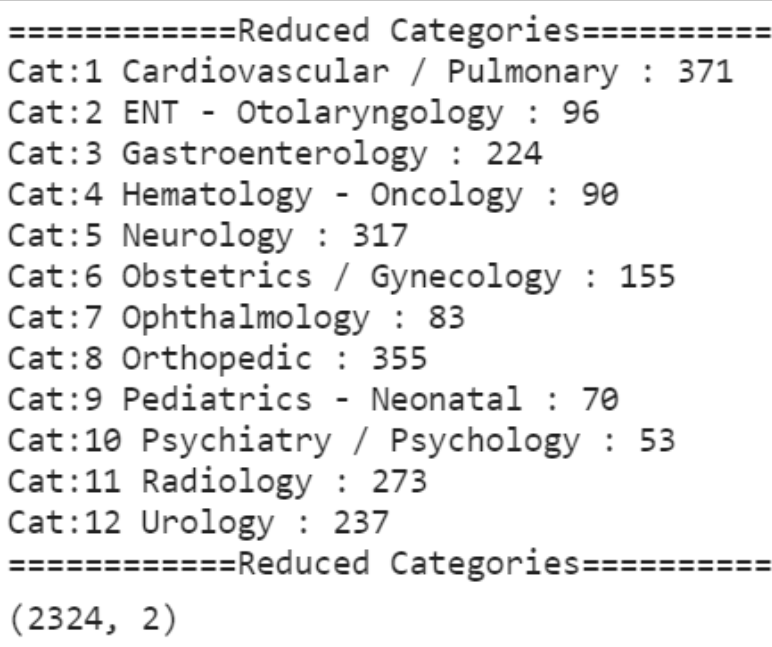
\includegraphics[width=\textwidth,height=7cm,keepaspectratio]{pictures/5.4reducedCat(12cat).png} 
% \caption{Το πλήθος εγγραφών ανά κατηγορία μετά την απαλοιφή και τη συγχώνευση κάποιων κατηγοριών}\label{figure5.5}
% \end{figure}


% Το \en{sciSpacy} είναι ένα πακέτο της  \en{Python} το οποίο περιέχει τα μοντέλα  \en{Spacy} και είναι σχεδιασμένο για προεπεξεργασία σε κείμενα που περιέχουν οντότητες που αποτελούν ιατρική, επιστημονική ή κλινική ορολογία.

% Αξιοποιώντας τη δυνατότητα αυτού του πακέτου, δημιουργείται η συνάρτηση \en{process\_text()} η οποία περνάει κάθε εγγραφή του πεδίου \en{transcription} ως είσοδο στη μέθοδο \en{nlp()} του μοντέλου \en{en\_ner\_bionlp13cg\_md} του πακέτου \en{sciSpacy}, η οποία επιστρέφει το σύνολο λέξεων που έχουν ιατρική, επιστημονική ή κλινική νοηματική αξία.


% Έπειτα, εφαρμόζουμε αναδρομικά όλη τη διαδικασία:
% \begin{enumerate}
%     \item Προεπεξεργασία (εφαρμογή \en{sciSpacy})
%     \item \en{Tf-Idf} αξιολόγηση
%     \item Απεικόνιση του πίνακα \en{Tf-Idf} με χρήση της μεθόδου \en{t-SNE}
%     \item Εφαρμογή \en{PCA} στον πίνακα \en{Tf-Idf}
%     \item Εκ νέου διαχωρισμός δεδομένων σε \en{training set} και \en{test set}
%     \item Εφαρμογή λογιστικής παλινδρόμησης \en{(logistic regression)}
%     \item Κατασκευή Πίνακα Σύγχυσης \en{(confusion matrix)}
%     \item Εμφάνιση νέων αποτελεσμάτων μετρικών ποιότητας πρόβλεψης
% \end{enumerate}

% Το Σχήμα~ \ref{figure5.6} εμφανίζει την απεικόνιση του πίνακα που προέκυψε από την \en{tf-idf} με χρήση της μεθόδου \en{t-SNE} μετά την εκ νέου προεπεξεργασία των δεδομένων 

% \begin{figure} [ht!]
% \centering
% 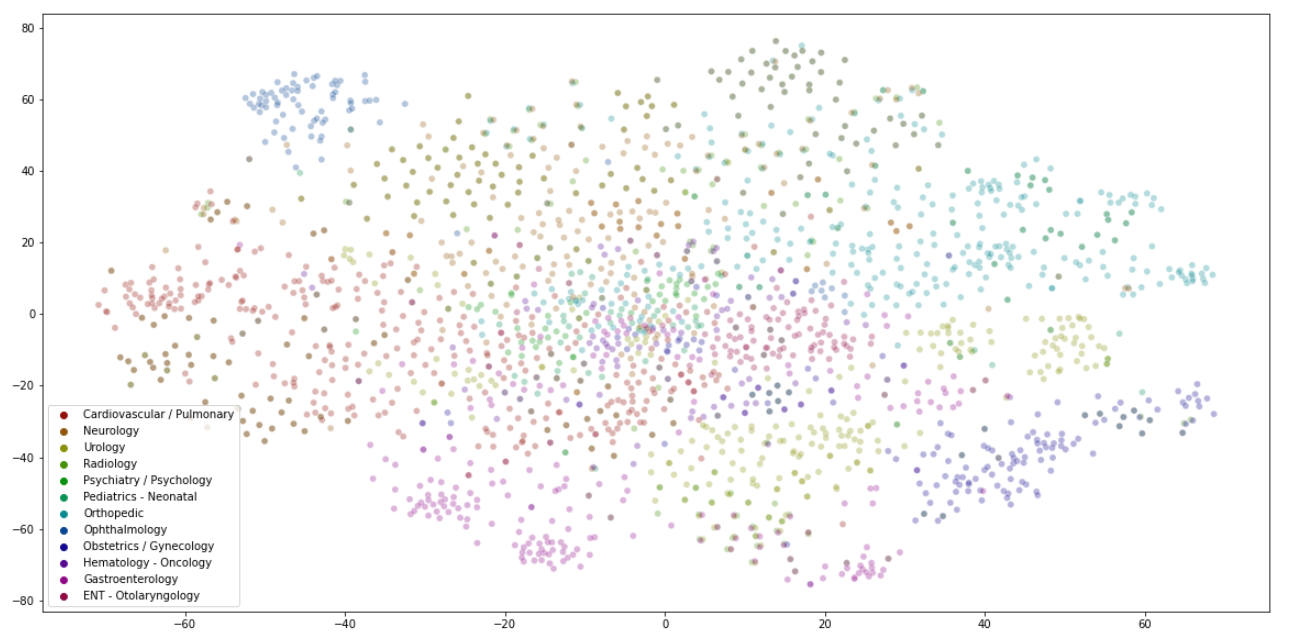
\includegraphics[width=\textwidth,height=12cm,keepaspectratio]{pictures/5.6tsne2.png} 
% \caption{Η νέα γραφική απεικόνιση του αλγορίθμου \en{t-SNE}}\label{figure5.6}
% \end{figure}


% Ο νέος Πίνακας Σύγχυσης και ο νέος Πίνακας αποτελεσμάτων μετρικών ταξινόμησης φαίνονται στα σχήματα ~\ref{figure5.7} και ~\ref{figure5.8}

% \begin{figure} [ht!]
% \centering
% 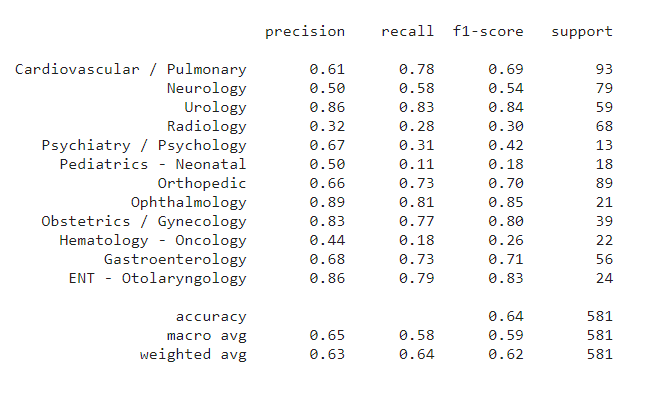
\includegraphics[width=\textwidth,height=8cm,keepaspectratio]{pictures/5.8results2.png} 
% \caption{Πίνακας Αποτελεσμάτων μετρικών ταξινόμησης μετά την επεξεργασία με το πακέτο \en{sciSpacy}}\label{figure5.8}
% \end{figure}

% \begin{figure} [ht!]
% \centering
% 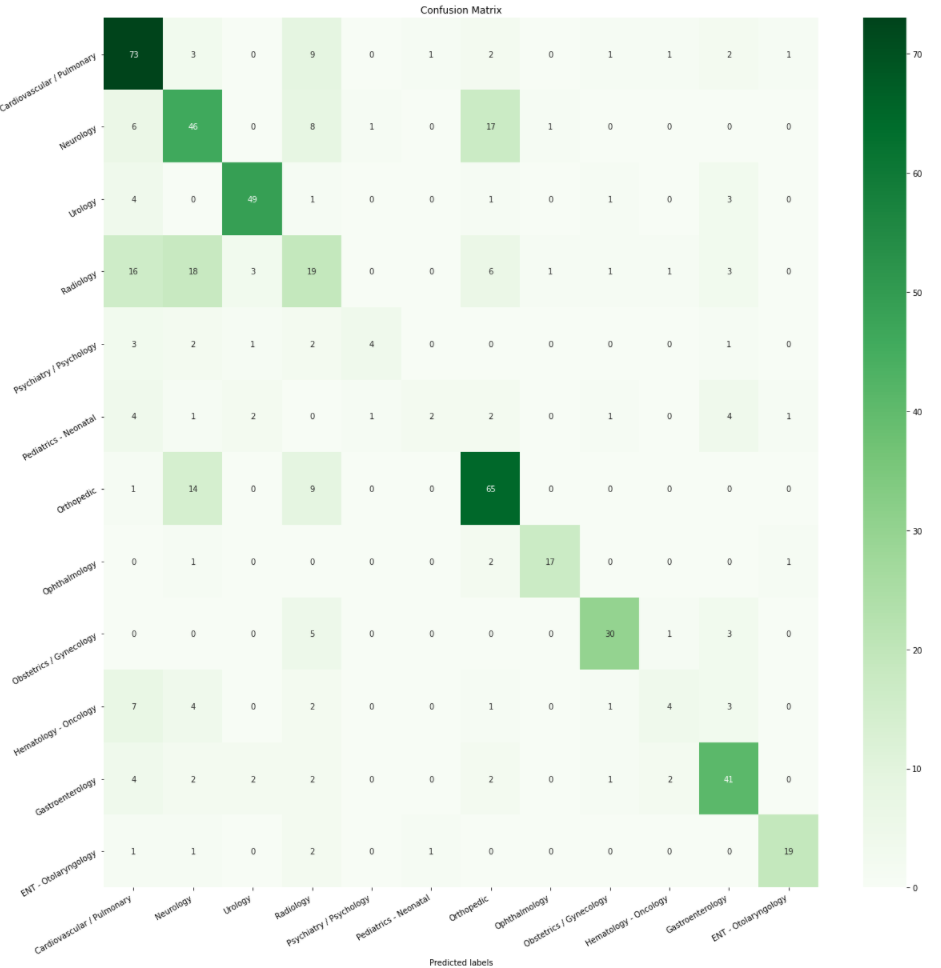
\includegraphics[width=\textwidth,height=12cm,keepaspectratio]{pictures/5.7cMatrix2.png} 
% \caption{Πίνακας Σύγχυσης  μετά την επεξεργασία με το πακέτο \en{sciSpacy}}\label{figure5.7}
% \end{figure}
% \clearpage

% Παρατηρούμε εμφανώς βελτιωμένα αποτελέσματα στα \en{scores} των διάφορων μετρικών. (προηγούμενα αποτελέσματα στο σχήμα ~\ref{figure5.4})
% Παρ’ όλα αυτά, εξακολουθεί να υπάρχει ανισορροπία στο πλήθος των υπαρχόντων δεδομένων μεταξύ των κατηγοριών. 

% Στα πλαίσια της συγκεκριμένης εργασίας ακολουθήθηκαν σε προηγούμενα βήματα και οι δύο προσεγγίσεις αντιμετώπισης της ανισορροπίας των δεδομένων \en{(oversampling} και \en{undersampling}: αφαιρέθηκαν οι κλάσεις που αποτελούσαν μειονότητες καθώς και η κλάση της χειρουρικής που περιείχε δεδομένα κατά πολύ μεγαλύτερα σε όγκο σε σχέση με τις υπόλοιπες κλάσεις τα οποία επίσης συγχέονταν με αυτές λόγω επικαλυπτόμενων γνωστικών πεδίων.

% Μία ακόμα απλή προσέγγιση για την αντιμετώπιση του προβλήματος θα ήταν να χρησιμοποιηθεί η απλούστερη \en{oversampling} τεχνική η οποία υποδεικνύει τη δημιουργία διπλότυπων στιγμιοτύπων στις κατηγορίες που αποτελούν μειονότητες. Κάτι τέτοιο όμως, παρ' ότι φαινομενικά επιφέρει μεγαλύτερη ισορροπία στα δεδομένα, δεν προσθέτει καμία καινούρια πληροφορία στο μοντέλο εκπαίδευσης.

% Γι' αυτό θα χρησιμοποιηθεί η τεχνική \en{SMOTE (Synthetic Minority Oversampling Technique)}.


% Πριν τη δημιουργία νέου \en{dataset} με την τεχνική \en{SMOTE} τα δεδομένα ήταν τα εξής:
% \en{
% \begin{itemize}
%     \item Train\_Set\_Size: (1743, 696)
%     \item Test\_Set\_Size: (581, 696) 
% \end{itemize}}


% Μετά τη δημιουργία νέου \en{dataset} με την τεχνική \en{SMOTE} τα δεδομένα είναι τα εξής:
% \en{
% \begin{itemize}
%     \item Train\_Set\_Size: (1981, 696)
%     \item Test\_Set\_Size: (661, 696) 
% \end{itemize}
% }

% \clearpage 
% \section{Λογιστική Παλινδρόμηση }

% Στη συνέχεια γίνεται εφαρμογή Λογιστικής Παλινδρόμησης και παράγεται ο νέος Πίνακας Σύγχυσης (Σχήμα ~ \ref{figure5.10}):

% \begin{figure} [ht!]
% \centering
% 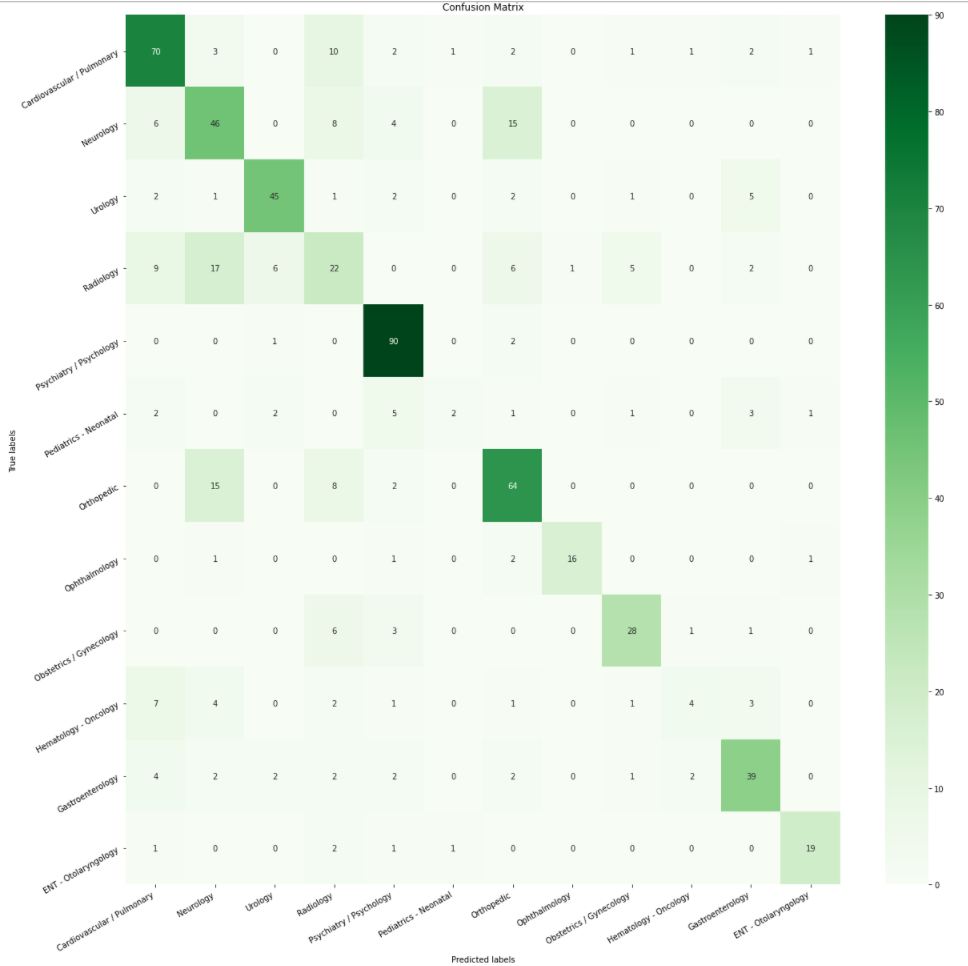
\includegraphics[width=\textwidth,height=12cm,keepaspectratio]{pictures/5.10CMatrix3.png} 
% \caption{Πίνακας Σύγχυσης μετά την εφαρμογή της τεχνικής \en{SMOTE}}\label{figure5.10}
% \end{figure}

% \clearpage
% Τέλος, δημιουργείται ο πίνακας των τελικών αποτελεσμάτων μετρικών ταξινόμησης ο οποίος φαίνεται στο σχήμα ~\ref{figure5.11}.

% \begin{figure} [ht!]
% \centering
% 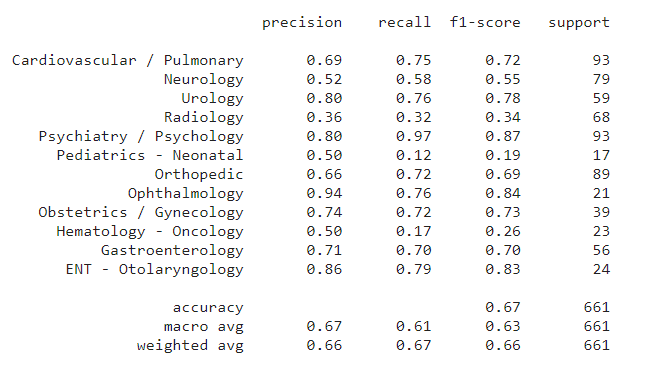
\includegraphics[width=\textwidth,height=8cm,keepaspectratio]{pictures/5.11results3.png} 
% \caption{\en{Logistic Regression: }Πίνακας τελικών Αποτελεσμάτων μετρικών ταξινόμησης μετά την εφαρμογή της τεχνικής \en{SMOTE}}\label{figure5.11}
% \end{figure}

% Τα τελικά αποτελέσματα είναι εμφανώς βελτιωμένα. 
% Παρατηρούμε οτι σε συγκεκριμένες κατηγορίες όπως \en{Neurology, Radiology} και \en{Hematology} τα αποτελέσματα ταξινόμησης παραμένουν χαμηλά καθώς οι περιγραφές των περιστατικών εξακολουθούν να αφορούν παραπάνω απο μία ειδικότητες. 


% Στη συνέχεια, για την ταξινόμηση του κειμένου, δοκιμάζεται η επίδοση των αλγορίθμων:
% \begin{enumerate}
%     \item \en{Naïve Bayes} 
%     \item \en{SVM}
%     \item \en{kNN}
% \end{enumerate}


% διατηρώντας ως είσοδο το \en{dataset} στην τελευταία μορφή που ταξινομήθηκε με τη μέθοδο της λογιστικής παλινδρόμησης, πριν την επεξεργασία για επίτευξη \en{oversampling} με την τεχνική \en{SMOTE}.

% \clearpage
% \section{Αλγόριθμος \en{Naïve Bayes}}
% Ο πίνακας αποτελεσμάτων των μετρικών ταξινόμησης που παράγεται από τη μέθοδο \en{classification\_report()} για τον Αλγόριθμο \en{Naïve Bayes} φαίνεται στο σχήμα ~\ref{figure5.12}.

% \begin{figure} [ht!]
% \centering
% 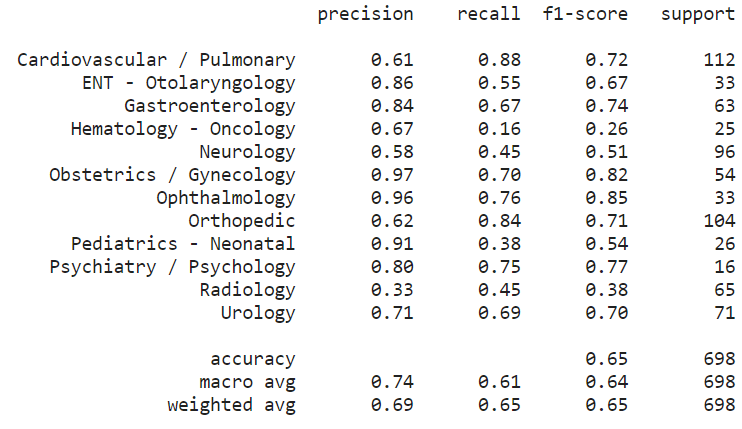
\includegraphics[width=\textwidth,height=8cm,keepaspectratio]{pictures/NAiveBAyes_NO_SMOTE.png} 
% \caption{\en{Naïve Bayes: }Πίνακας Αποτελεσμάτων μετρικών ταξινόμησης}\label{figure5.12}
% \end{figure}
% \clearpage

% \section{Αλγόριθμος \en{SVM}}

% Ο πίνακας αποτελεσμάτων των μετρικών ταξινόμησης που παράγεται από τη μέθοδο \en{classification\_report()} για τον Αλγόριθμο \en{SVM} φαίνεται στο σχήμα ~\ref{figure5.13}.

% \begin{figure} [ht!]
% \centering
% 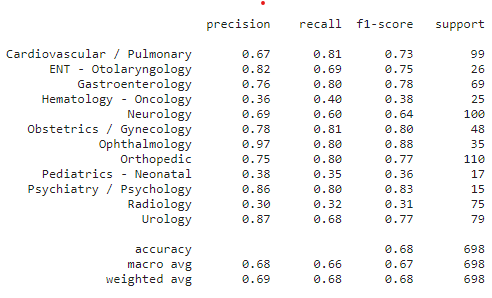
\includegraphics[width=\textwidth,height=8cm,keepaspectratio]{pictures/SVM_NO_SMOTE.png} 
% \caption{\en{SVM: }Πίνακας Αποτελεσμάτων μετρικών ταξινόμησης}\label{figure5.13}
% \end{figure}
% \clearpage

% \section{Αλγόριθμος \en{kNN}}
% Ο πίνακας αποτελεσμάτων των μετρικών ταξινόμησης που παράγεται από τη μέθοδο \en{classification\_report()} για τον Αλγόριθμο \en{kNN} φαίνεται στο σχήμα ~\ref{figure5.14}.

% \begin{figure} [ht!]
% \centering
% 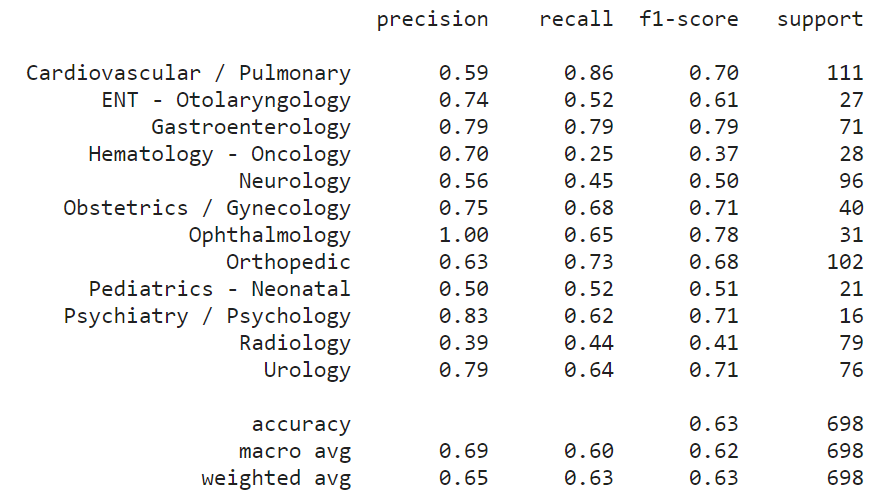
\includegraphics[width=\textwidth,height=8cm,keepaspectratio]{pictures/knn_NO_SMOTE.png} 
% \caption{\en{kNN: }Πίνακας Αποτελεσμάτων μετρικών ταξινόμησης}\label{figure5.14}
% \end{figure}




% \section{\en{Word2Vec - Neural Network}}





	\chapter{Επίλογος}

\section{Αποτελέσματα}

Συγκεντρωτικά, τα αποτελέσματα όλων των μεθόδων φαίνονται στον παρακάτω πίνακα: 

\setlength{\arrayrulewidth}{0.5mm}
\setlength{\tabcolsep}{18pt}
\renewcommand{\arraystretch}{1.5}
\begin{table}[h]
    \centering
    \begin{tabular}{  | l | c | }
    \hline
    \multicolumn{2}{|c|}{Πίνακας Αποτελεσμάτων} \\
    \hline
    Αλγόριθμος & Ακρίβεια \\
    \hline
    \en{Logistic Regression} & 0.64 \\
    \en{Logistic Regression \& SMOTE} & 0.67 \\
    \en{Naive - Bayes} & 0.65\\
    \en{K Nearest Neighbors (KNN)} & 0.63\\
    \en{Support Vector Machines (SVM)} & 0.67\\
    \en{Word2Vec \& Neural Network}  & 0.68  \\
    \hline
    \end{tabular}
    \caption{Συγκεντρωτικός Πίνακας Αποτελεσμάτων Ακρίβειας}
\end{table}

\section{Συμπεράσματα}

Συμπερασματικά, το συγκεκριμένο \en{dataset} δεν είναι εύκολο να επεξεργαστεί με ακρίβεια καθώς δεν είναι «καθαρό».
Με διάφορες τεχνικές φτάνουμε σε καλύτερα αποτελέσματα, ωστόσο αυτό δεν ειναι εφικτό να εφαρμοστεί σωστά σε οποιαδήποτε περιγραφή περιστατικού.

Mέσα από τις διάφορες προσεγγίσεις, με διαφορετική αναπαράσταση δεδομένων και διαφορετικές τεχνικές, καταφέραμε να φτάσουμε σε κάποια ικανοποιητικά ποσοστά ακρίβειας. 

Το μεγαλύτερο ίσως εμπόδιο για την επίτευξη αυτού του στόχου ήταν η αντιμετώπιση της ανισορροπίας των δεδομένων, δηλαδή η άνιση κατανομή τους στις διάφορες κλάσεις, η επικάλυψη των κλάσεων, η σωστή προεπεξεργασία των κειμένων ώστε να απομονωθεί η χρήσιμη πληροφορία και η σωστή παραμετροποίηση του νευρωνικού δικτύου για την αποτελεσματική εκπαίδευση του μοντέλου. 

\section{Μελλοντικές Επεκτάσεις}
Ωστόσο, τα ποσοστά ακρίβειας που επιτεύχθησαν, αποτελούν αισιόδοξο σημάδι για μελλοντική δουλειά. Δημιουργώντας στο μέλλον ένα πιο ισορροπημένο και ακριβές \en{dataset}, θα μπορέσουμε να εκπαιδεύσουμε καλύτερα το σύστημα μας ωστε να αναπτύξουμε ένα ακόμα πιο ισχυρό και αποτελεσματικό εργαλείο.
Πέρα από την πρόβλεψη ιατρικής ειδικότητας, μέσα απο την περιγραφή ιατρικού περιστατικού θα μπορούσε να δημιουργηθεί πρόγνωση για το μέτρο του επείγοντος, τη φαρμακευτική περίθαλψη που ενδεχομένως χρειστεί ή την πιθανότητα να χρειαστεί εισαγωγή και νοσηλεία, αντικείμενα και αποφάσεις που απασχολούν ιατρικό προσωπικό χωρίς απαραίτητα να χρήζουν ιατρικών γνώσεων. 

Εν κατακλείδι, η δημιουργία χρήσιμων, ισχυρών και αποτελεσματικών εργαλείων στα χέρια ιατρών, ερευνητών και επιστημόνων αποτελεί ένα πεδίο με μεγάλο φάσμα προκλήσεων και προς επίλυση προβλημάτων, στοχεύοντας πάντα στην υποστήριξη και όχι στην αντικατάσταση επιστημονικά καταρτισμένου προσωπικού. 


	\include{body_matter/chap7}
% Βιβλιογραφία - Αναφορές
	\bibliography{back_matter/references}

%%%%%%%%%%%%%%%%%%%%%%%%%%%%%%%%%%%%%%%%%%%%%%%%%%%%
\backmatter
% Ευρετήριο Όρων
	\printindex
	\cleardoublepage
	\pagebreak
	\thispagestyle{empty}
\end{document}